
\documentclass[12pt,a4]{article}

\usepackage[utf8]{inputenc}
\usepackage[T1]{fontenc}
\usepackage{amsmath, amssymb, amsfonts}
\usepackage{mathtools}
\usepackage{graphicx, float, epstopdf}
\usepackage{enumerate}
\usepackage{bm}
\usepackage[noabbrev]{cleveref}
\usepackage{caption}
\DeclareMathOperator*{\argmin}{\arg\!\min}

\newcommand{\R}{{\mathbb R}}
\newcommand{\C}{{\mathbb C}}
\newcommand{\N}{{\mathbb N}}
\newcommand{\ra}{\rightarrow}
\newcommand{\lra}{\longrightarrow}
\newcommand{\lnorm}{\left\|}
\newcommand{\rnorm}{\right\|}
\newcommand{\ind}{{\mathbf{1}}}

\newcommand{\citeneeded}{\ensuremath{\vphantom{1}^{\text{[citation needed]}}\,}}
\newcommand{\eps}{\ensuremath{\varepsilon}}
\newcommand{\vc}[1]{\ensuremath{\bm{#1}}}
\newcommand*{\bigCI}{%
  \mathrel{\text{%
    {\rotatebox[origin=c]{90}{\resizebox{2.25ex}{1.65ex}{$\vDash$}}}%
  }}%
}


\title{Glottal inversion with approximate vocal tract filter}
\author{Lasse Lybeck, Robert Sirviö}


\begin{document}

\maketitle

%---------------------Introduction--------------------
\section{Introduction}
\label{sec:intro}

A synthetic human vowel sound consists of a periodic signal to simulate the glottal excitation signal at the glottis and a filter to simulate the vocal tract, which the glottal signal is filtered through.\cite{touda} With a given vocal tract filter the direct problem is \emph{given a glottal excitation signal, create the vowel sound}. The inverse problem is \emph{given a (recorded) vowel sound, find the glottal excitation signal}. In this study we will be concentrating on the inverse problem using simulated vowel data.

The inversion from a vowel sound to the glottal signal is an important part of creating synthetic human voices and speech generators. To create a synthetic vowel both the glottal signal and the vocal tract filter are needed. However, the glottal signal cannot be directly measured, but it can be approximated with inversion of a recorded vowel. With this data models for simulating the glottal excitation signal can be created.


%-----------------Materials & Methods-----------------
\section{Materials and Methods}
\label{sec:methods}

\subsection{Glottal excitation signal}
\label{sec:rk}

In this study the Rosenberg-Klatt model (RK-model) for the glottal excitation signal will be used for the generation of synthetic data and as a reference point for the obtained results. The RK-model is a simple model for the glottal signal, proposed in 1970 by Rosenberg.\cite{rosenberg} The model is simple and easy to use, as it creates the signal only from two parameters, the sound frequency $f$ and the so called Klatt-parameter $Q$.

The \emph{airflow} for the glottal excitation signal created by the RK-model is defined as
\begin{equation}
\label{eq:RK-model}
g(t) =
  \begin{cases}
   at^2 + bt^3  & \text{if } 0 \leq t \leq Q T \\
   0            & \text{if } Q T < t \leq T,
  \end{cases}
\end{equation}
where $t$ is a time variable, $T = 1/f$ is the period of the pitch, $Q \in \left[ 0,1 \right]$ is the Klatt-parameter and $a$ and $b$ are variables defined in terms of $T_0 := QT$ as
\begin{equation*}
a = \frac{27}{4 T_0^2}, \quad b = -\frac{27}{4 T_0^3} .
\end{equation*}
Here the parameter $f$ defines the frequency of the generated signal and the Klatt-parameter $Q$ defines the shape of the pulse.

The glottal excitation signal can be retrieved as the derivative $g'$ of the airflow function. Here $g'$ is the \emph{pressure function}, and simulates the sound generated in the glottis. The pulse generated by the model can be seen in figure \ref{fig:klatt}.

Another, more widely used, model for the glottal excitation signal worth mentioning is the Liljencrants-Fant model (LF-model).\cite{fant} It is regarded as more accurate than the RK-model, but it is also much more complex. It has also been shown, that the LF-model generates only marginally better approximations for the resulting vowel after the vocal tract filtering than the RK-model.\cite{fujisaki} Due to this and the overall complexity of the LF-model we will be using the RK-model for the simulation of the glottal excitation signal in this study.

\begin{figure}[t]
\begin{center}
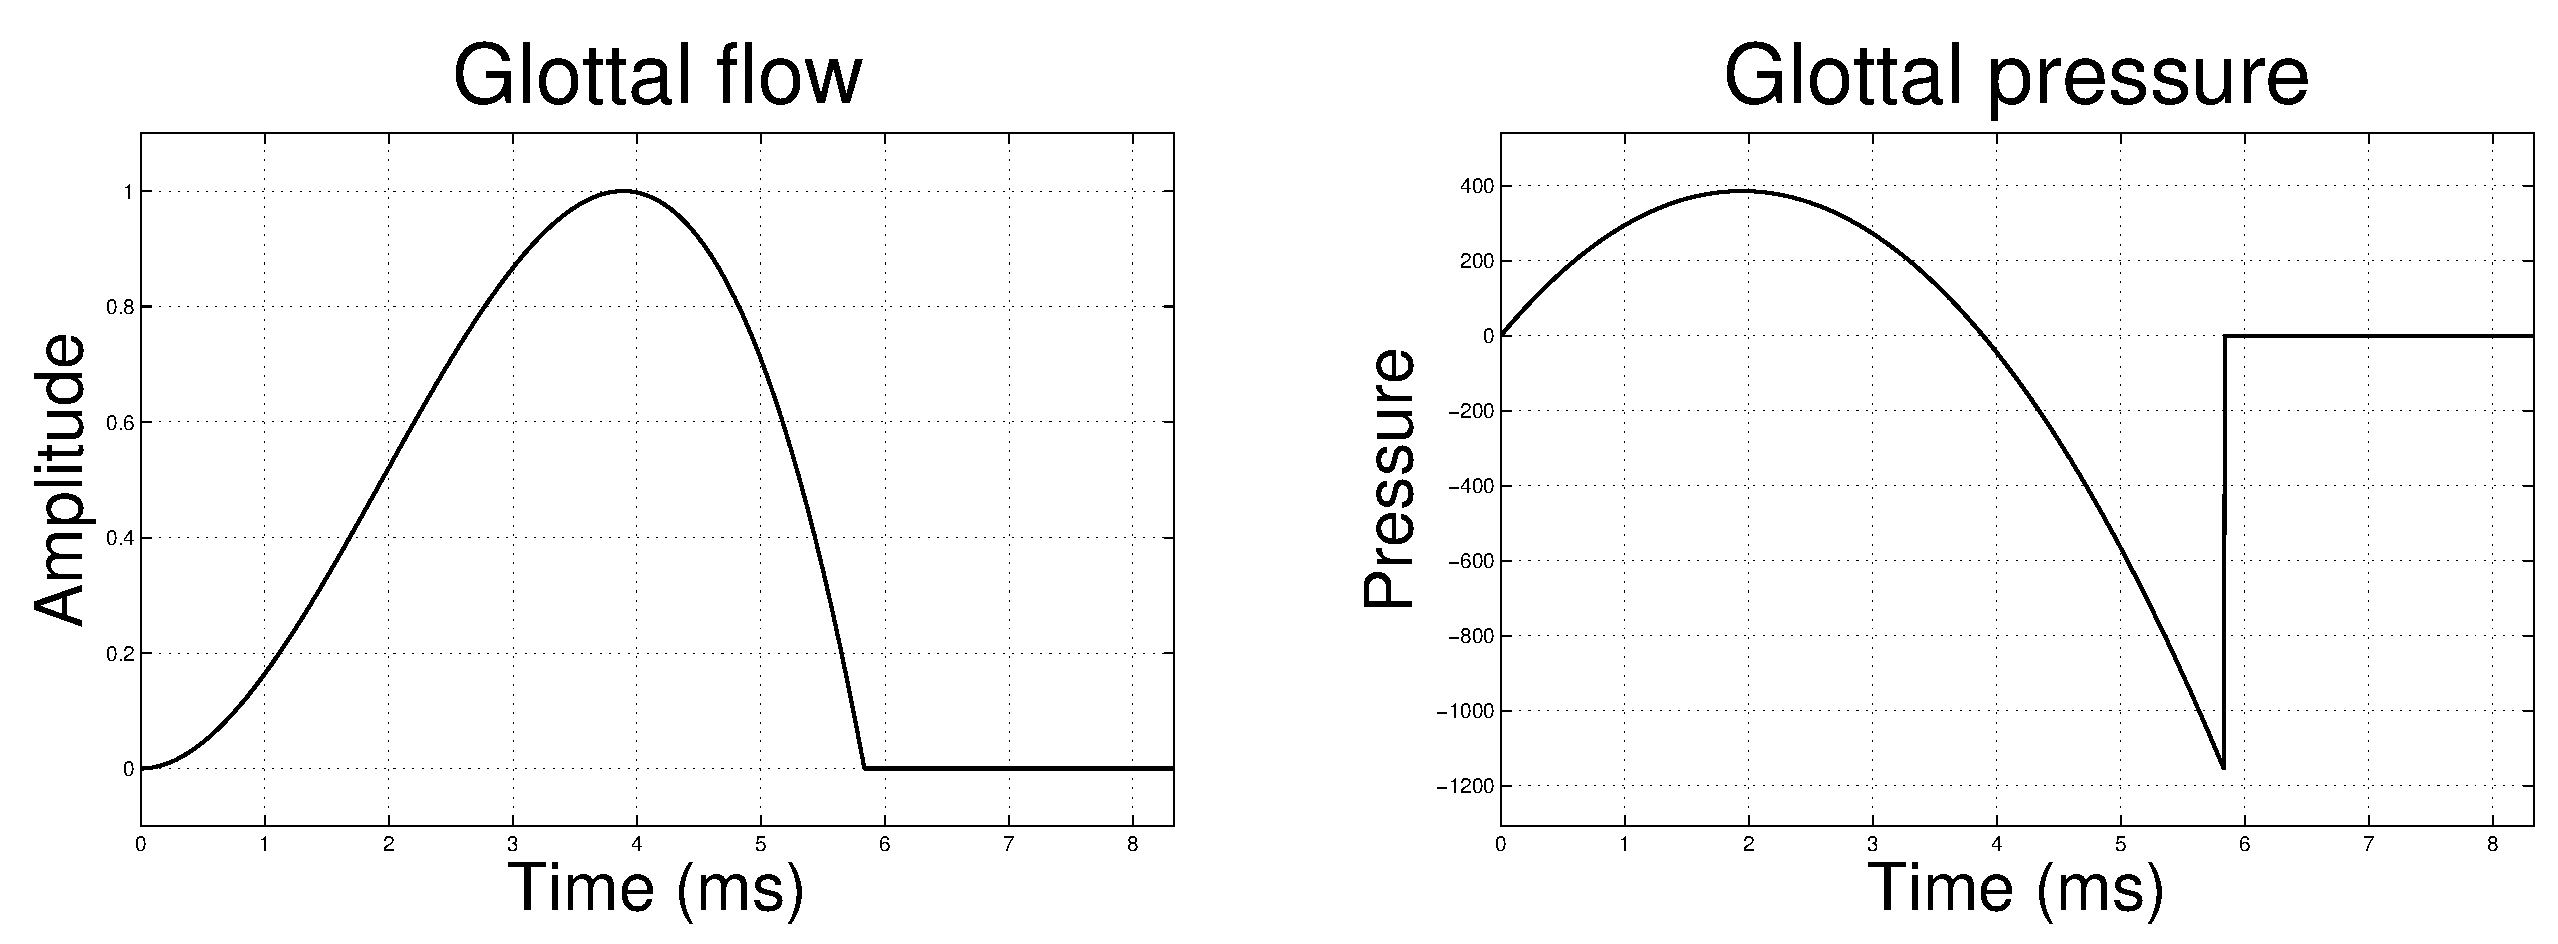
\includegraphics[width=.8\textwidth]{img/klatt.eps}
\end{center}
\caption{The airflow and pressure generated by the RK-model}
\label{fig:klatt}
\end{figure}


\subsection{Vocal tract filter}
\label{sec:filter}

In this study we will assume an approximate vocal tract filter to be known for the recorded vowel we want to invert. The digital filter, defined by a vector $\vc{a} = \left( a_1, a_2, \ldots , a_{N_a} \right)^T \in \R^{N_a}$, filters the data $\vc{x} = \left( x_1, x_2, \ldots , x_n \right)^T \in \R^n$ as defined by the difference equation
\begin{equation}
\left\{
\begin{alignedat}{1}
\label{eq:filter-diffeq}
y_1     &= x_1 \\
a_1 y_j &= -\sum_{k=2}^{\min\{j-1, N_a\}} a_{k} y_{j-k} ,
\end{alignedat}
\right.
\end{equation}
where $\vc{y} = \left( y_1, y_2, \ldots , y_n \right) \in \R^n$ is the filtered data. We denote $\vc{y} = \varphi_{\vc{a}} (\vc{x})$.

Consider now the filter defined by $\vc{a} \in \R^{N_a}$ and the data $\vc{x} \in \R^n$ which we want to filter. Now the filter defined by \eqref{eq:filter-diffeq} can be expressed by the the matrix $A \in \R^{n \times n}$, where
\begin{equation}
\label{eq:filter-matrix}
\left\{
\begin{alignedat}{3}
   &A_{1,1}     = a_1 \\
   &A_{i,1}     = - \sum_{k=1}^{\min\{ i-1, N_a-1 \}} a_{k+1} A_{i-k,1}, \quad && 2 \leq i \leq n \\
   &A_{i+1,j+1} = A_{i,j},     && j \leq i \\
   &A_{i,j}     = 0,           && j > i .
\end{alignedat}
\right.
\end{equation}
Now $\varphi_{\vc{a}} (\vc{x}) = A \vc{x}$.


\subsection{The matrix model}
\label{sec:matrixModel}

A vowel sound can be simulated by applying a digital filter $A \in \R^{n \times n}$, defined as in \eqref{eq:filter-matrix}, to a sample of a glottal excitation signal $\vc{g} \in \R^n$ as
\begin{equation}
\label{eq:vow}
\vc{v} = A \vc{g} .
\end{equation}
Here $\vc{v} \in \R^n$ is the simulated vowel.

In this study we will assume an approximation of the filter $A$ to be known. Given the measurements $\vc{m} \in \R^n$ of a vowel corresponding approximately to the filter $A$, equation \eqref{eq:vow} can be expressed as
\begin{equation}
\label{eq:vowModel}
\vc{m} = A \vc{g} + \vc{\eps},
\end{equation}
where $\vc{\eps} \in \R^n$ denotes the measurement noise.


\subsection{The inversion method}
\label{sec:invMethod}

\subsubsection{Tikhonov reguralization}
\label{sec:tikh}
The classical Tikhonov regularized solution for $\vc{m} = A \vc{g} + \vc{\eps}$, defined in section \ref{sec:matrixModel}, is usually denoted by the vector $T_\alpha( \vc{m} ) \in \R^n$ that minimizes
\begin{equation*}
\lnorm AT_\alpha( \vc{m} ) - \vc{m} \rnorm^2 + \alpha \lnorm T_\alpha( \vc{m} ) \rnorm^2 \Leftrightarrow
\end{equation*}
\begin{equation*}
T_\alpha( \vc{m} ) = \underset{ \vc{z} \in \R^n}{\argmin}
\left\{ \lnorm A \vc{z} - \vc{m} \rnorm^2 + \alpha \lnorm \vc{z} \rnorm^2 \right\},
\end{equation*}
where $\alpha > 0$ is called a regularization parameter. The resulting $T_\alpha( \vc{m} )$ can be understood as a compromise between two conditions, namely
\begin{enumerate}[I.]
 \item $T_\alpha( \vc{m} )$ should give a small residual $AT_\alpha( \vc{m} ) - \vc{m}$.
 \item $\lnorm T_\alpha( \vc{m} ) \rnorm_2$ should be small.
\end{enumerate}
The $\alpha$ parameter is used in order to tune to balance between the two conditions above.

In generalized Tikhonov regularization some prior knowledge is assumed to be known. For example, in some cases $g$ might be known to be smooth. This information can be incorporated into the regularization by choosing
\begin{equation}
T_\alpha( \vc{m} ) = \underset{\vc{z} \in \R^n}{\argmin}
\left\{ \lnorm A \vc{z} - m \rnorm^2 + \alpha \lnorm L \vc{z} \rnorm^2 \right\},
\end{equation}  
where $L$ is a discretized differential operator. As shown in \cite{samu}, the regularized solution satisfies
\begin{equation}
\label{eq:tik-normal}
\left( A^T A + \alpha L^T L \right) T_{\alpha}( \vc{m} ) = A^T \vc{m} ,
\end{equation}
which can be used to calculate the solution numerically.
 
In our model proposed in section \ref{sec:rk} we know the airflow of the excitation signal to be smooth in the interval $[0, QT]$ and to be zero in the interval $]QT, T]$. This can be incorporated in our model by customizing the discrete differential operator matrix, described in more detail in section \ref{sec:basis}.


\subsubsection{The conjugate gradient method}
\label{sec:conjgrad}

The conjugate gradient method is an iterative method for the quadratic optimization problem
\begin{equation}
\label{eq:quad-optim}
\text{minimize } \frac{1}{2} \vc{x}^T Q \vc{x} - \vc{b}^T \vc{x} ,
\end{equation}
where $Q \in \R^{n \times n}$ is a symmetric positive definite matrix. We will now briefly explain the algorithm and its use to our particular problem. For a more detailed explanation, see \cite{samu}.

Let $\vc{b} \in \R^n$ fixed, $Q \in \R^{n \times n}$ a symmetric positive definite matrix, $\vc{x_0} \in \R^n$ the initial guess and define $\vc{d_0} = -\vc{g_0} = \vc{b} - Q \vc{x_0}$. Now for $k \geq 0$ let
\begin{equation}
\begin{alignedat}{3}
&\alpha_k      &&= -\frac{\vc{g_k}^T \vc{d_k}}{\vc{d_k}^T Q \vc{d_k}} \\
&\vc{x_{k+1}}  &&= \vc{x_k} + \alpha_k \vc{d_k} \\
&\vc{g_{k+1}}  &&= Q \vc{x_{k+1}} - \vc{b} \\
&\beta_k       &&= \frac{\vc{g_{k+1}}^T Q \vc{d_k}}{\vc{d_k}^T Q \vc{d_k}} \\
&\vc{d_{k+1}}  &&= -\vc{g_{k+1}} + \beta_k \vc{d_k} .
\end{alignedat}
\end{equation}
Now $\vc{x_k}$ converges toward the solution of \eqref{eq:quad-optim}. We now want to apply the conjugate gradient algorithm in the case of the optimization problem defined in \eqref{eq:tik-normal} for the Tikhonov regularization.

Let $A \in \R^{n \times n}$, $L \in R^{n \times n}$ invertible and $\alpha > 0$. Now the square matrix $B := A^T A + \alpha L^T L$ is invertible. If we denote $\vc{f} := T_\alpha ( \vc{m} )$ in \eqref{eq:tik-normal}, the problem becomes to minimize the expression
\begin{equation}
\label{eq:conjgrad-basis}
\lnorm B \vc{f} - A^T \vc{m} \rnorm^2 .
\end{equation}

We see that
\begin{equation}
\label{eq:conjgrad-calc}
\begin{alignedat}{1}
\lnorm B \vc{f} - A^T \vc{m} \rnorm^2
  &= \left< B \vc{f}, B \vc{f} \right> - 2 \left< B \vc{f}, A^T \vc{m} \right> + \left< A^T \vc{m}, A^T \vc{m} \right> \\
  &= \vc{f}^T B^T B \vc{f} - 2 \vc{m}^T A B \vc{f} + \lnorm A^T \vc{m} \rnorm^2 .
\end{alignedat}
\end{equation}
Further, we notice that $B^T B$ is a positive definite symmetric matrix, since
\begin{equation*}
\vc{v}^T (B^T B) \vc{v} = (B \vc{v})^T B \vc{v} = \lnorm B \vc{v} \rnorm^2 > 0
\end{equation*}
for any $\vc{v} \in R^n$, $\vc{v} \neq 0$, due to the fact that $B$ is invertible. Now we define
\begin{equation*}
Q := 2 B^T B \quad \text{and} \quad \vc{b}^T := 2 \vc{m}^T A B .
\end{equation*}
As can be seen from \eqref{eq:conjgrad-calc}, minimizing \eqref{eq:conjgrad-basis} is equivalent to minimizing the expression
\begin{equation}
\frac{1}{2} \vc{f}^T Q \vc{f} - \vc{b}^T \vc{f} ,
\end{equation}
and thus we can use the conjugate gradient method for the optimization.



\subsubsection{Morozov's discrepancy principle}
\label{sec:morozov}
The problem of finding the optimal regularization parameter is, in general, considered to be unsolved. There are, however, methods that attempt to find an optimal choice of the regularization parameter, including the Morozov discrepancy principle, which is based on the noise level in the data.

Assume that we know the size of the noise in our model defined by \eqref{eq:vowModel} to be $\delta > 0$. Now $T_\alpha( \vc{m} )$ is an acceptable reconstruction if 
\begin{equation}
\lnorm AT_\alpha( \vc{m} )- \vc{m} \rnorm \leq \delta \quad \left( A \in R^{k \times n}\right).
\end{equation}
The idea of the Morozov's discrepancy principle is to choose $\alpha > 0$ such that
\begin{equation}
\lnorm AT_\alpha( \vc{m} ) - \vc{m} \rnorm = \delta
\end{equation}
It can be proven (see \cite{samu}) that the $\alpha$ that satisfies the above expression is attained by solving
\begin{equation}\label{eq:morozov_root}
\sum_{j=1}^{\min\left\{ k,n \right\}} \left( \frac{\alpha}{d_j^2 + \alpha} \right)^2 \left( m'_j \right)^2 + \sum_{j = \min\left\{k,n\right\} + 1}^k \left( m'_j \right)^2 - \delta^2 = 0,
\end{equation}
where $d_j$ are the singular values of $A$ and $\vc{m'} = U^T \vc{m}$ where $U$ is an orthogonal matrix acquired from the singular value decomposition $A = U D V^T$.

As previously mentioned, we will use Morozov's discrepancy principle to choose the optimal regularization parameter.

\subsection{The basis and materials}
\label{sec:basis}

In this work we will mainly use synthetic data as our basis (for real data, see section \ref{sec:realData}). We first create a synthetic glottal excitation signal using the airflow function defined in \eqref{eq:RK-model}. To this signal we apply a previously calculated vocal tract filter, as described in section \ref{sec:filter} to create a simulated vowel sound. Finally we add some normally distributed noise to the data to simulate measurement noise. Different data is created by varying the sound frequency, the value of the Klatt-parameter $Q$ and the noise-level.

The inversion of the vowel sound is done using another filter similar to the one used in creating the synthetic data. For example we might have created the data with a filter for a male vowel /a/, and use a filter for a female vowel /a/ for the inversion. This way we avoid inverse crime. The idea is that we can assume two different filters for the same vowel to be approximately the same. That is, given two different filters $A_1$ and $A_2$ for the same vowel and a glottal excitation signal $\vc{g}$, we assume that $A_1 \vc{g} \approx A_2 \vc{g}$. This is based on the fact that a vowel is defined by its two or three first \emph{formant frequencies}, which can be assumed to be about the same for two different vowel sounds.\cite{digitalmodels}

We then attempt to solve the inverse problem by using the generalized Tikhonov regularization with a customized penalty matrix. We will assume the Klatt-parameter $Q$ of the glottal excitation signal to be known (at least approximately), and as explained in section \ref{sec:rk} we know the pressure function to be zero in the interval $]QT, T]$. This will be incorporated in the model by assigning large values to the diagonal entries $l_i \in L$ for the values of $i$ that correspond to the previously mentioned interval, namely $i \in \left\{ j \in \N : Qn < j \leq n \right\}$ where $n$ is the length of our data. We also know the pressure function to be smooth in the interval $[0, Q]$. This can be incorporated by adding differential operator properties to the penalty matrix.

We can thus assign the differential operator properties
\begin{equation*}
\begin{cases}
 l_{i,i}   &= 1 \\
 l_{i,i+1} &= -1 
\end{cases}
\text{ when } i \in \left\{ j \in \N : 1 \leq j \leq Qn \right\} ,
\end{equation*}
and further, we assign the larger values described above as
\begin{equation*}
 l_{i,i} = C \geq 1, \quad \text{when } i \in \left\{ j \in \N : Qn < j \leq n \right\}
\end{equation*}
resulting in the penalty matrix
\begin{equation}
L=
\begin{pmatrix*}[c]
 1      & -1     &  0     & 0       &    &    & \cdots  &        & 0       \\
 0      & 1      & -1     & 0       &    &    & \cdots  &        & 0       \\
 \vdots &        & \ddots & \ddots  &    &    &         &        & \vdots  \\
 0      & \cdots &  0     & 1       & -1 & 0  & 0       & \cdots & 0       \\
 0      & \cdots &  0     & 0       & C  & 0  & 0       & \cdots & 0       \\
 0      & \cdots &  0     & 0       & 0  & C  & 0       & \cdots & 0       \\
 \vdots &        &        &         &    &    & \ddots  &        & \vdots  \\
 0      &        &        & \cdots  &    &    &  0      &  C     & 0       \\
 0      &        &        & \cdots  &    &    &  0      &  0     & C 
\end{pmatrix*}
\end{equation}
for a single period of the excitation signal. This procedure must of course be repeated as many times as we have periods in our measurement data.

\subsubsection{Real data}
\label{sec:realData}

Apart from the synthetic data the method of inversion was also tested with real recorded data. As real data we will use recordings of the vowel /a/ in different pitches by different male subjects.

\subsubsection{Noise estimation}
\label{sec:noiseEst}

As previously mentioned, we will use Morozov's discrepancy principle for optimization of the regularization parameter $\alpha$. We assume the noise to originate from a scaled standard multivariate normal distribution, i.e. if
\begin{equation}
\vc{\eps'} = \left(Z_1, \ldots, Z_n \right), \quad Z_i \sim N(0,1) \bigCI \text{ for all }
i \in \left\{1, \ldots, n\right\}
\end{equation}
then our assumed noise vector is a sample from $\vc{\eps}$, defined as
\begin{equation}
\vc{\eps} := c \vc{\eps'} = \left(cZ_1, \ldots, cZ_n \right), \quad c > 0.
\end{equation}
Note that
\begin{equation}
cZ_i \sim N\left(0,c^2\right) \text{ for all }
i \in \left\{1, \ldots, n\right\}.
\end{equation}
The scaling is done to make the error relative to the data, which again is preferable in order to generate consistent data. We want to estimate the magnitude of the noise. Let $X \sim \chi_n^2$ and $Y \sim \chi_n$ where $\chi_n^2$ denotes the chi-squared distribution and $\chi_n$ the chi distribution with $n$ degrees of freedom respectively. We now see (\cite{handbook}, \cite{chi}) that
\begin{align*}
E\left(\lnorm \vc{\eps} \rnorm \right)   &= E\left(\lnorm c \vc{\eps'} \rnorm \right)   =
E\left(c \lnorm \vc{\eps'} \rnorm \right) = c E\left(\lnorm \vc{\eps'} \rnorm \right) \\
&= c E\left(\sqrt{Z_1^2 + \ldots + Z_n^2} \right) = c E\left(\sqrt{X} \right) \\
&= c E\left( Y \right) = 
c \sqrt{2}\frac{\Gamma\left(\frac{n+1}{2}\right)}{\Gamma\left(\frac{n}{2}\right)},  
\end{align*}
so the natural choice of $\delta$ is
\begin{equation}\label{eq:delta_choice}
\delta = c \sqrt{2}\frac{\Gamma\left(\frac{n+1}{2}\right)}{\Gamma\left(\frac{n}{2}\right)}.
\end{equation}
This is numerically impossible to compute in a straightforward manner due to fast growth of the gamma function, so in practice we will use 
\begin{equation}\label{eq:alt_delta_choice}
\delta = c\sqrt{2} \exp\left[
\log\Gamma\left(\frac{n+1}{2}\right) -  \log\Gamma\left(\frac{n}{2}\right) \right]  
\end{equation}
where the $\log\Gamma$ function is, in our case, more numerically stable. Note that expressions \eqref{eq:delta_choice} and \eqref{eq:alt_delta_choice} are equivalent.

In our case we know our approximated vocal tract filter to be at least to some extent erroneous. Therefore the measurement noise must be estimated somewhat differently to take the errors attained from the differences between the filters into account.

Let $\vc{m} \in \R^n$ be the given measurement data. As we know the sound frequency and the value of the Klatt-parameter we can generate a glottal excitation signal, and filter it with the approximated filter used in the inversion to create a similar vowel sound as our measurements. Let us denote it with $\vc{v} \in \R^n$. Now we can calculate an upper bound for the measurement noise as
\begin{equation}
\delta_{\text{max}} = \lnorm \vc{v} - \vc{m} \rnorm .
\end{equation}
However, we know our filter to be only an approximation of the filter used in generating the measurement data, not the exact same filter. Therefore it is reasonable to assume that the approximations done in the selection of the filter give rise to some differences in the vowel sound that cannot be regarded as measurement errors, but rather systematic errors attained by the approximations. Therefore we will use the estimation $\delta = \delta_{\text{max}} / 2$ for the noise level of the measurement data. This estimation of the measurement noise is not at all a trivial task, and should require more careful examination. This is however beyond the scope of this study.
 
When we have acquired an estimation for the measurement noise the solution of equation \eqref{eq:morozov_root} is approximated with Newton's method \cite{NR}.


\subsection{Approximation of the Klatt-parameter}
\label{sec:approxKlatt}

The inversion of the glottal sound is always done with a fixed guess of the Klatt-parameter $Q$. However, the real value of $Q$ can be approximated as long as the inversion is done with an approximation of $Q$ that is no less than what the data is created with. This means that we can approximate the Klatt-parameter as long as we always \emph{over-estimate} it a little bit.

The reason why we need to over-estimate the Klatt-parameter is the shape of the glottal excitation signal (see figure \ref{fig:klatt}). The negative peak in the glottal pressure is located at precisely the point $QT$ in time, where $T$ is the length of the period. The peak is quite sharp, and thus if the parameter is at all under-estimated the peak will almost completely vanish due to the inversion method suppressing the signal toward zero for all points after the time $QT$ (as explained in section \ref{sec:basis}).

When the inversion is done with a too large value of the parameter the result in the range $[0, QT]$ will give a good approximation for the signal, but the range $[QT, Q_{guess} T]$ will be very oscillatory although it should consist of zero values. The negative peak will, however, be clearly visible.  We can thus select the value for the next guess for $Q$ to be the point in the period where the least value is reached, plus a small constant to ensure that we still over-estimate the value. This procedure is then repeated.

As we always want to over-estimate the parameter we can start by selecting the initial guess $Q_1 = 1$. We then iterate for $i = 1, 2, \ldots, N$ the following. Solve the inverse problem as described in previous sections using $Q_i$ as the Klatt-parameter. Call the result $\vc{g}^{(i)} \in \R^n$. Next, find the index for the least value in $\vc{g}^{(i)}$, that is
\begin{equation*}
I_i = \argmin_{j \in \{1, \ldots, n\}} \vc{g}^{(i)}_j .
\end{equation*}
Then we get the new approximation for the Klatt-parameter simple by calculating $Q_{i+1} = I_i / n + c$, where $c > 0$ is a small constant.



%-----------------------Results-----------------------
\section{Results}
\label{sec:results}
\subsection{Results of the glottal inversion}
In this section we will present some of the results of our study. For obvious reasons we will not include sound data from our results in this paper. Note that in all the following graphs of the target glottal pressure and the reconstructed glottal pressure are represented by the colors green and blue, respectively. We will also denote the Klatt-parameter with $Q$. The relative errors of the reconstructions are calculated with the formula
\begin{equation}
\delta_{rel} = \frac{\left\| \vc{g} - T_{\alpha}(\vc{m}) \right\|_2}{\left\| \vc{g} \right\|_2} \cdot 100 \%,
\end{equation}
where $\vc{g} \in \R^k$ is the original glottal excitation signal and $T_{\alpha}(\vc{m})$ is the reconstruction calculated from the noisy data $m$ with the regularization parameter $\alpha$.

The inversion was done, in addition to the Tikhonov regularization strategy, also with the naïve inversion method in order to illustrate the ill-posedness of the inverse problem.
A comparison of the methods is presented below in figures \ref{fig:naive-comparison_crime} and \ref{fig:naive-comparison_nocrime}.
\begin{figure}[H]
\begin{center}
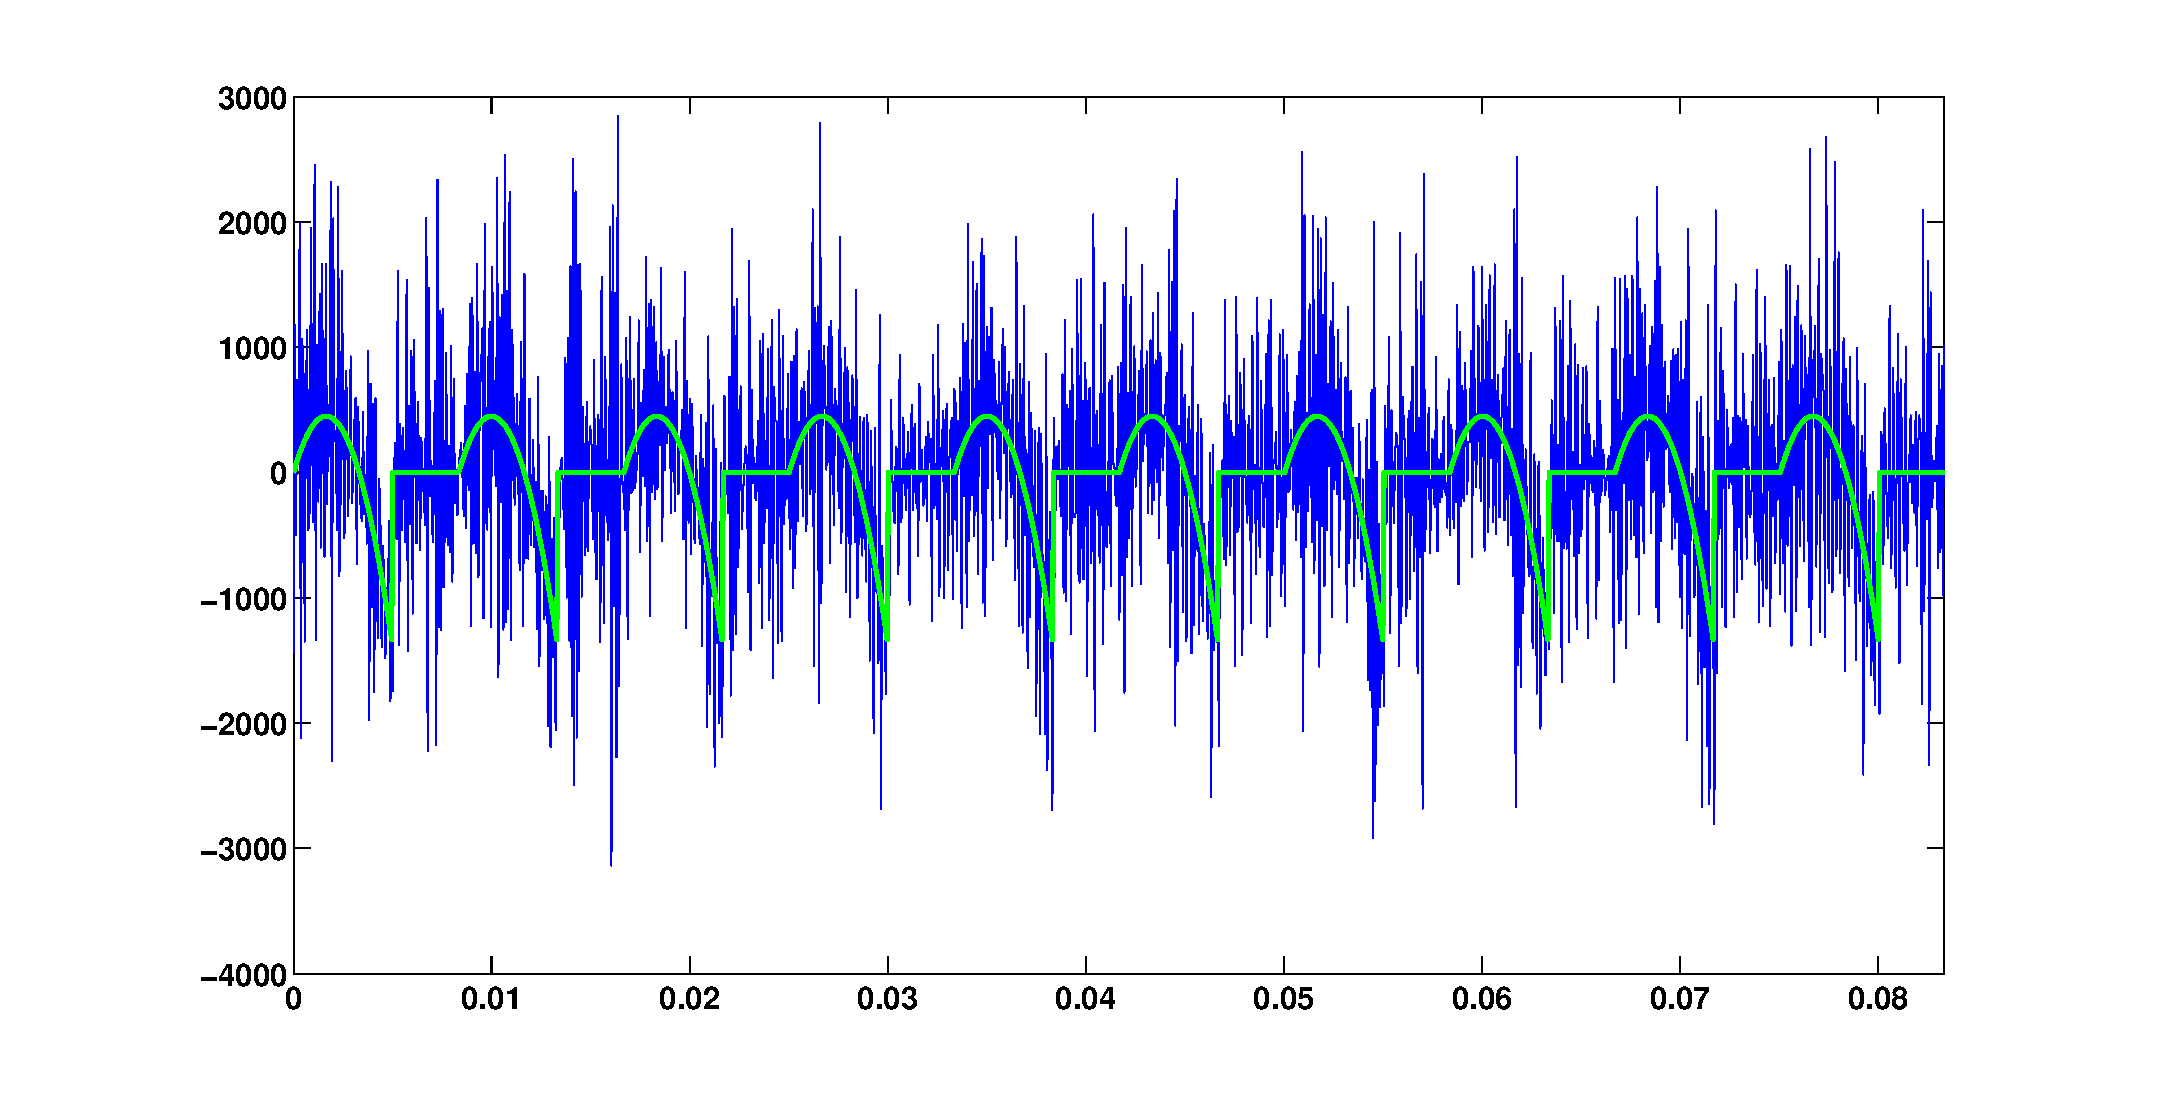
\includegraphics[scale=.3]{img/naive_test_naive.eps}
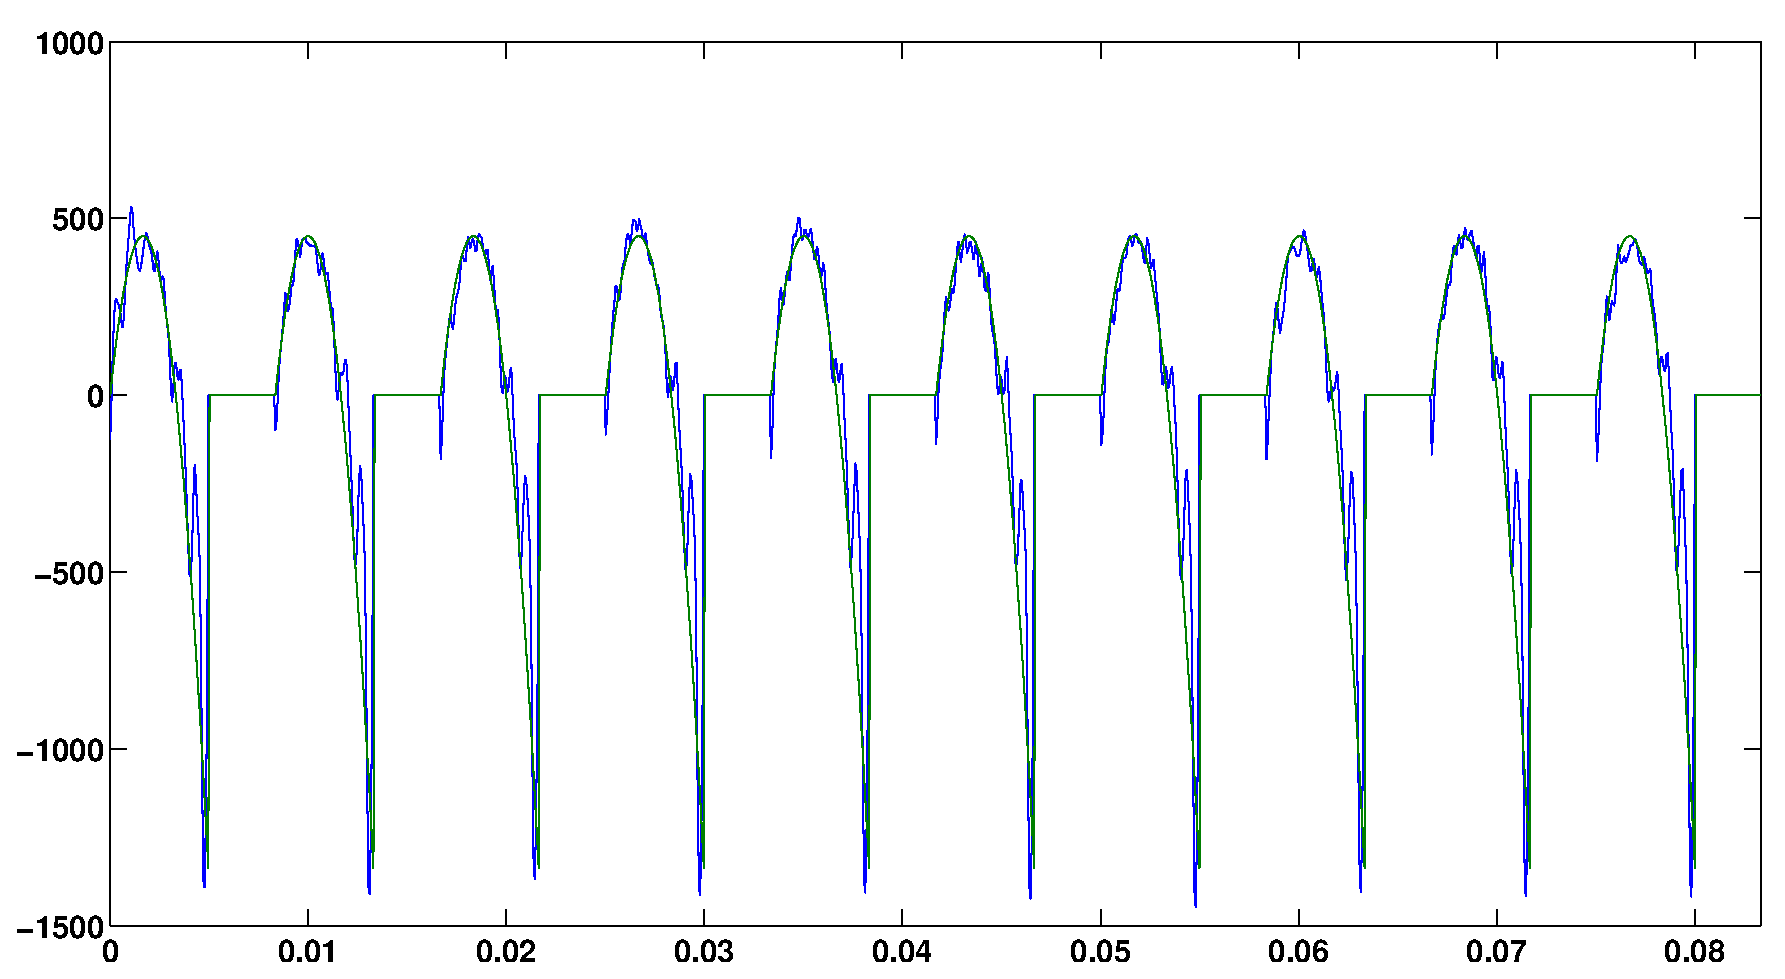
\includegraphics[scale=.3]{img/naive_test_morozov.eps}
\end{center}
\caption{Comparison between the naïve inversion method and the Tikhonov regularization strategy with inverse crime. Sound frequency = 90 Hz, Q = 0.7, relative error of the reconstruction $\approx$ 43.9\%, $\alpha \approx 63.7$.}
\label{fig:naive-comparison_crime}
\end{figure}

\begin{figure}[H]
\begin{center}
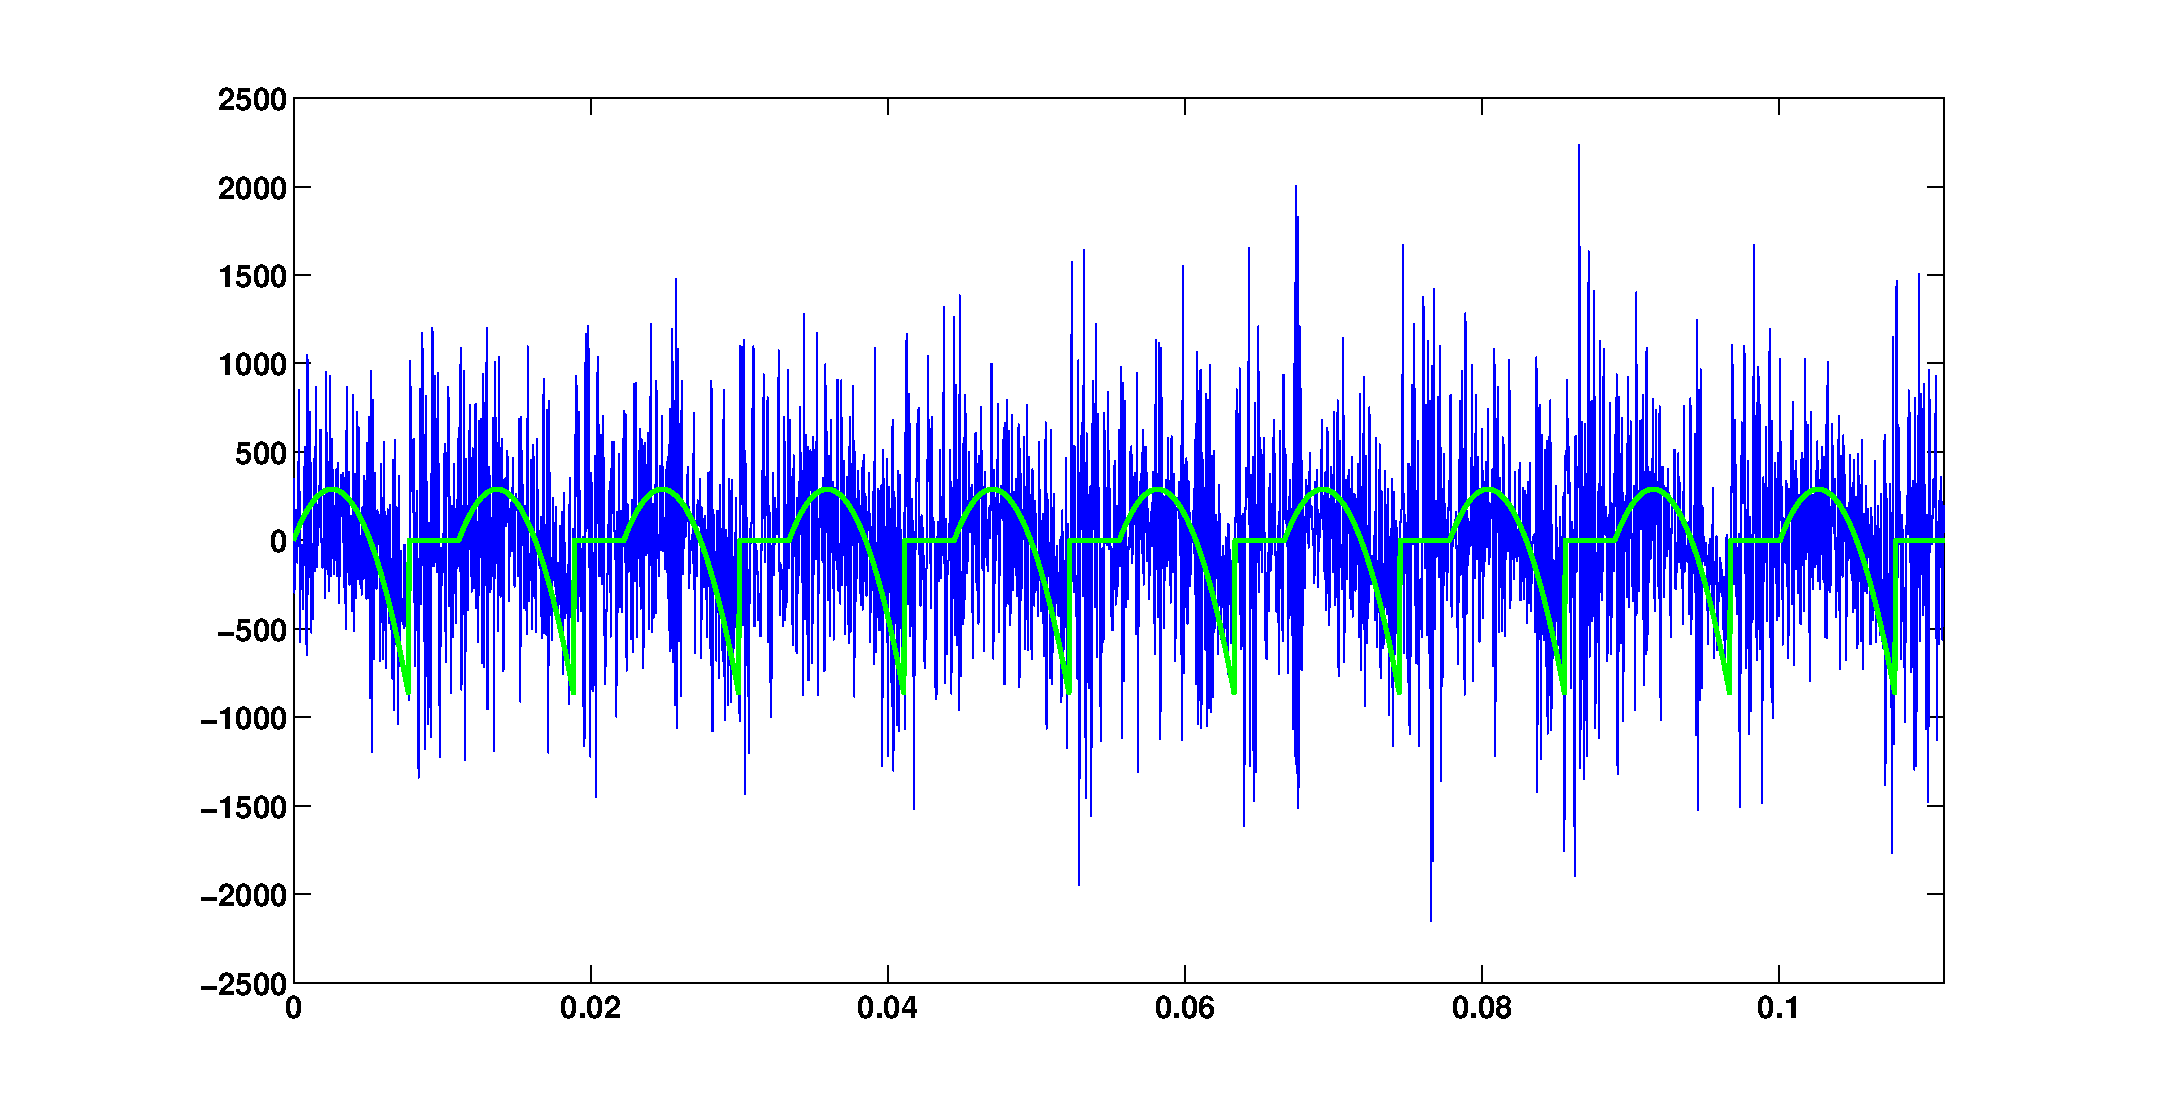
\includegraphics[scale=.3]{img/naive_test_naive[V3].eps}
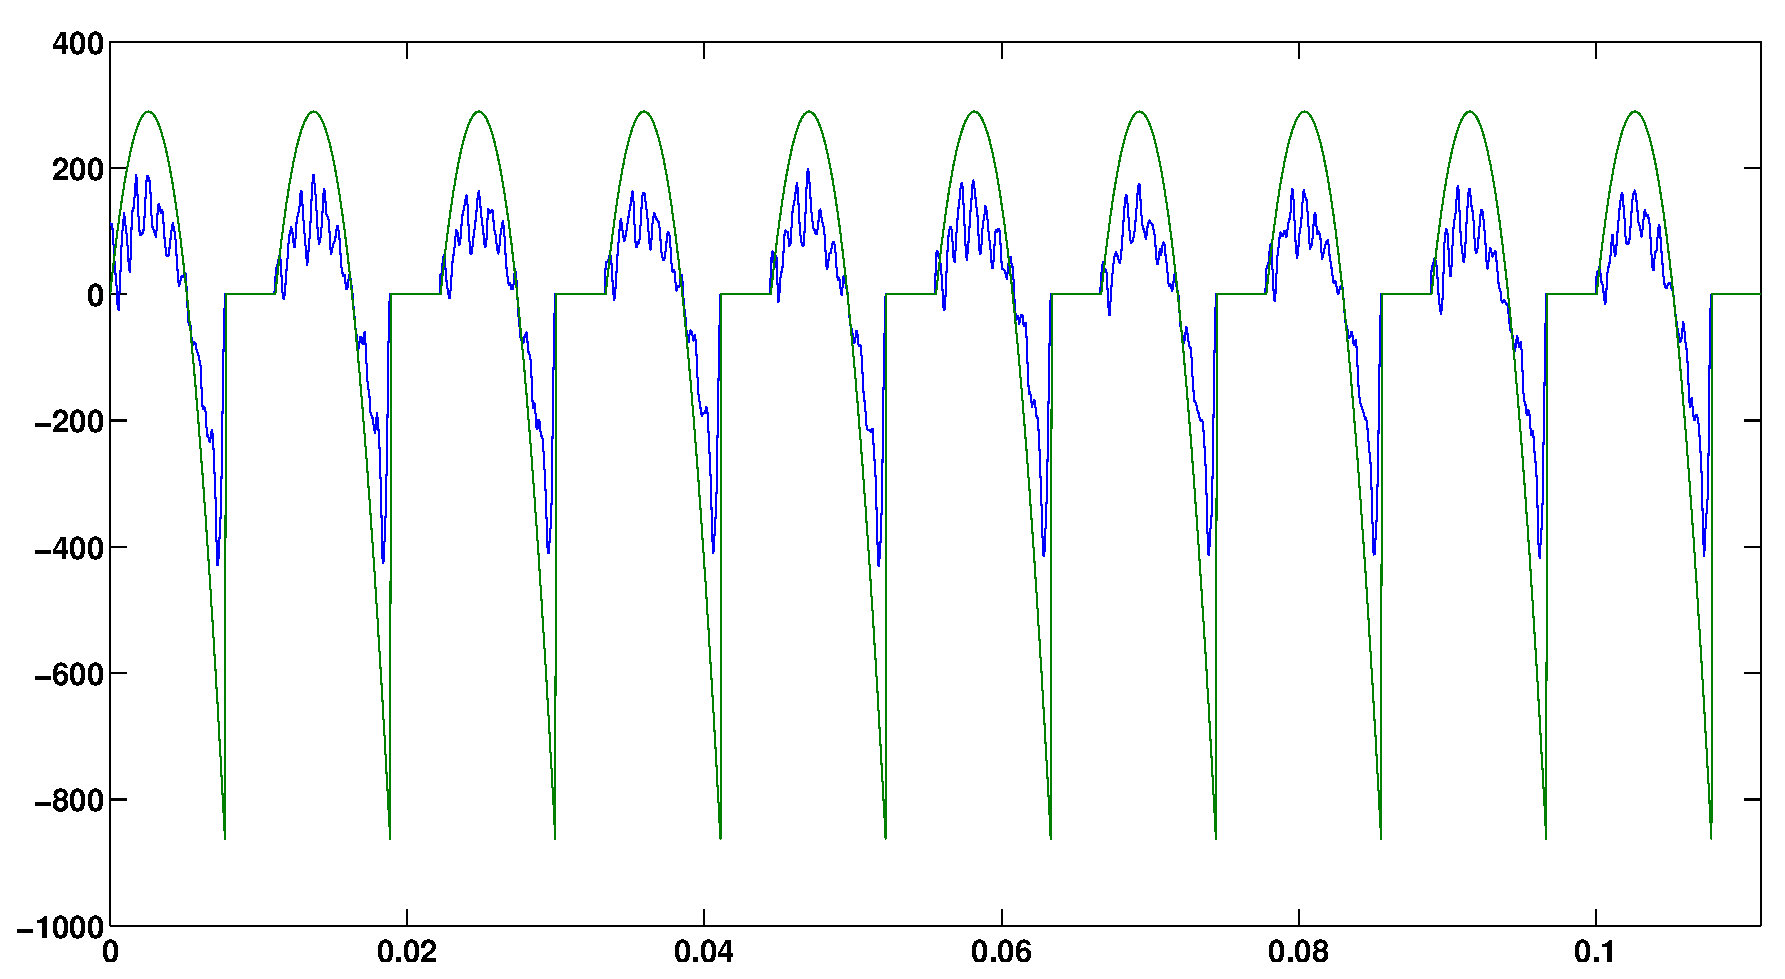
\includegraphics[scale=.3]{img/naive_test_morozov[V3].eps}
\end{center}
\caption{Comparison between the naïve inversion method and the Tikhonov regularization strategy without inverse crime. Sound frequency = 90 Hz, Q = 0.7, relative error of the reconstruction $\approx$ 63.1\%, $\alpha \approx 63.2$.}
\label{fig:naive-comparison_nocrime}
\end{figure}
In order to evaluate the accuracy and correctness (in the sense of the relative error of the glottal impulse) of the $\alpha$-value chosen according to Morozov's discrepancy principle the relative errors were calculated with different values of the parameters $\alpha$. This was then compared with corresponding reconstruction with an $\alpha$-value chosen according to Morozov's discrepancy principle. The results can be seen in figure \ref{fig:iter_comparison}.
\begin{figure}[H]
\begin{center}
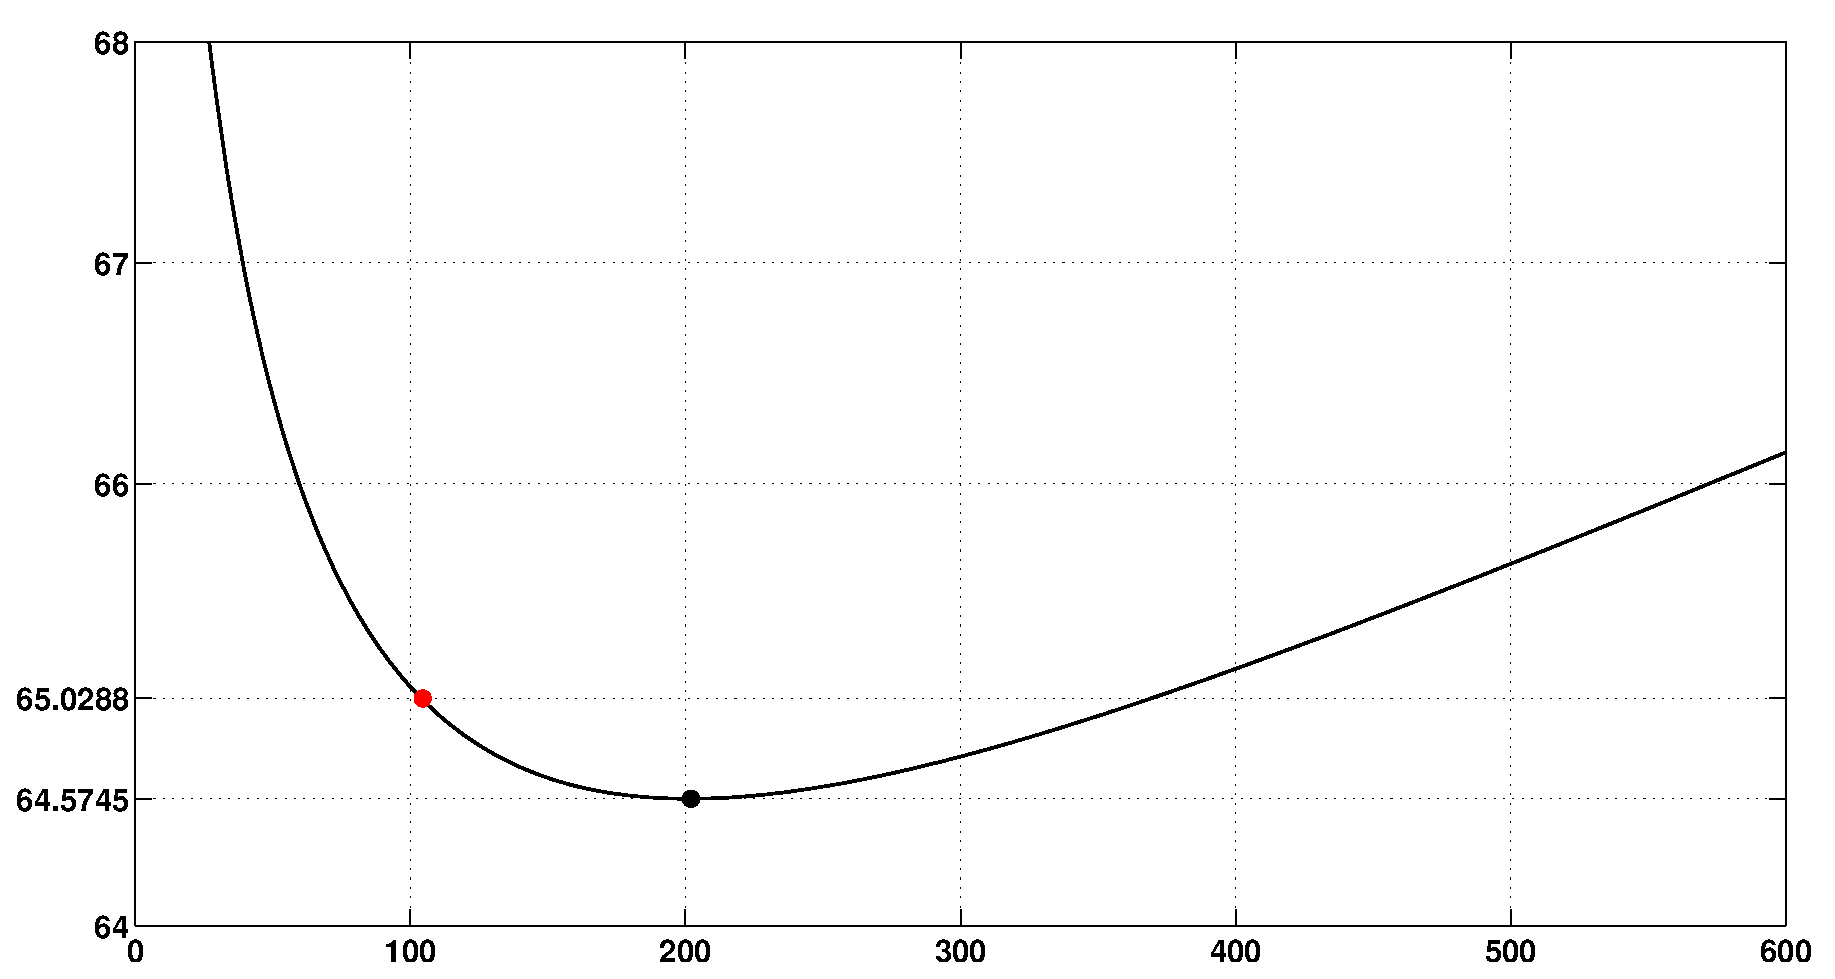
\includegraphics[scale=.3]{img/alpha_errs_iter.eps}
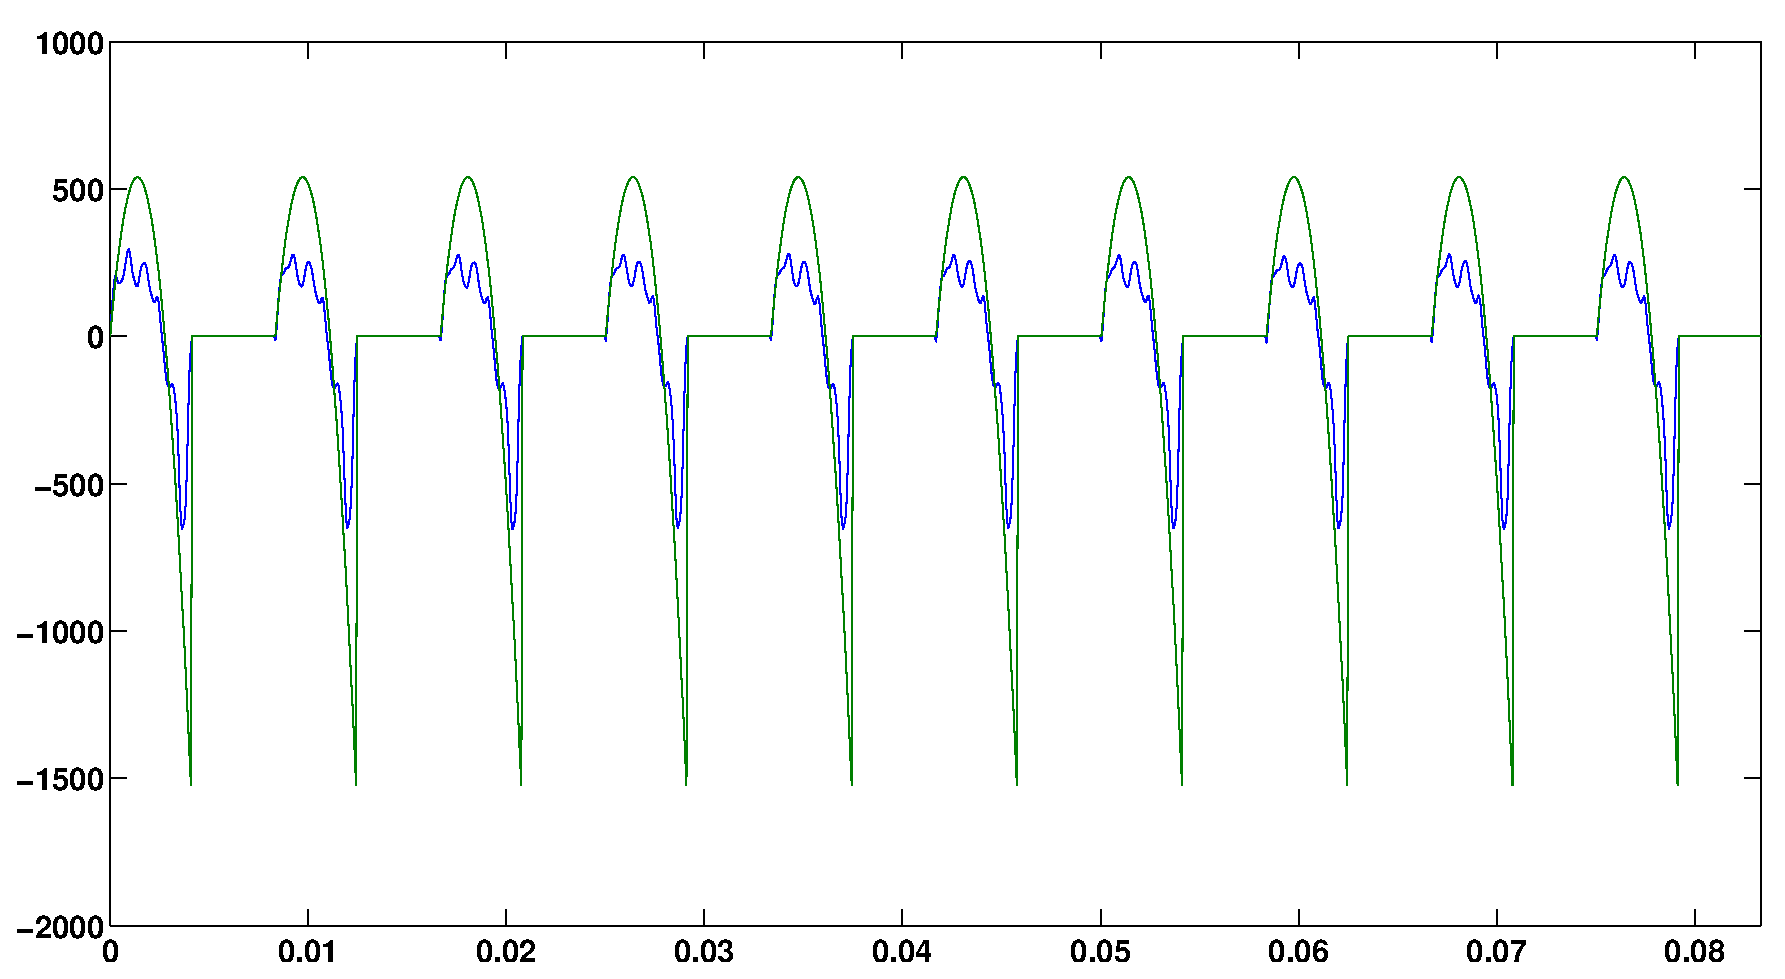
\includegraphics[scale=.3]{img/Comparison_with_iterative_nocrime.eps}
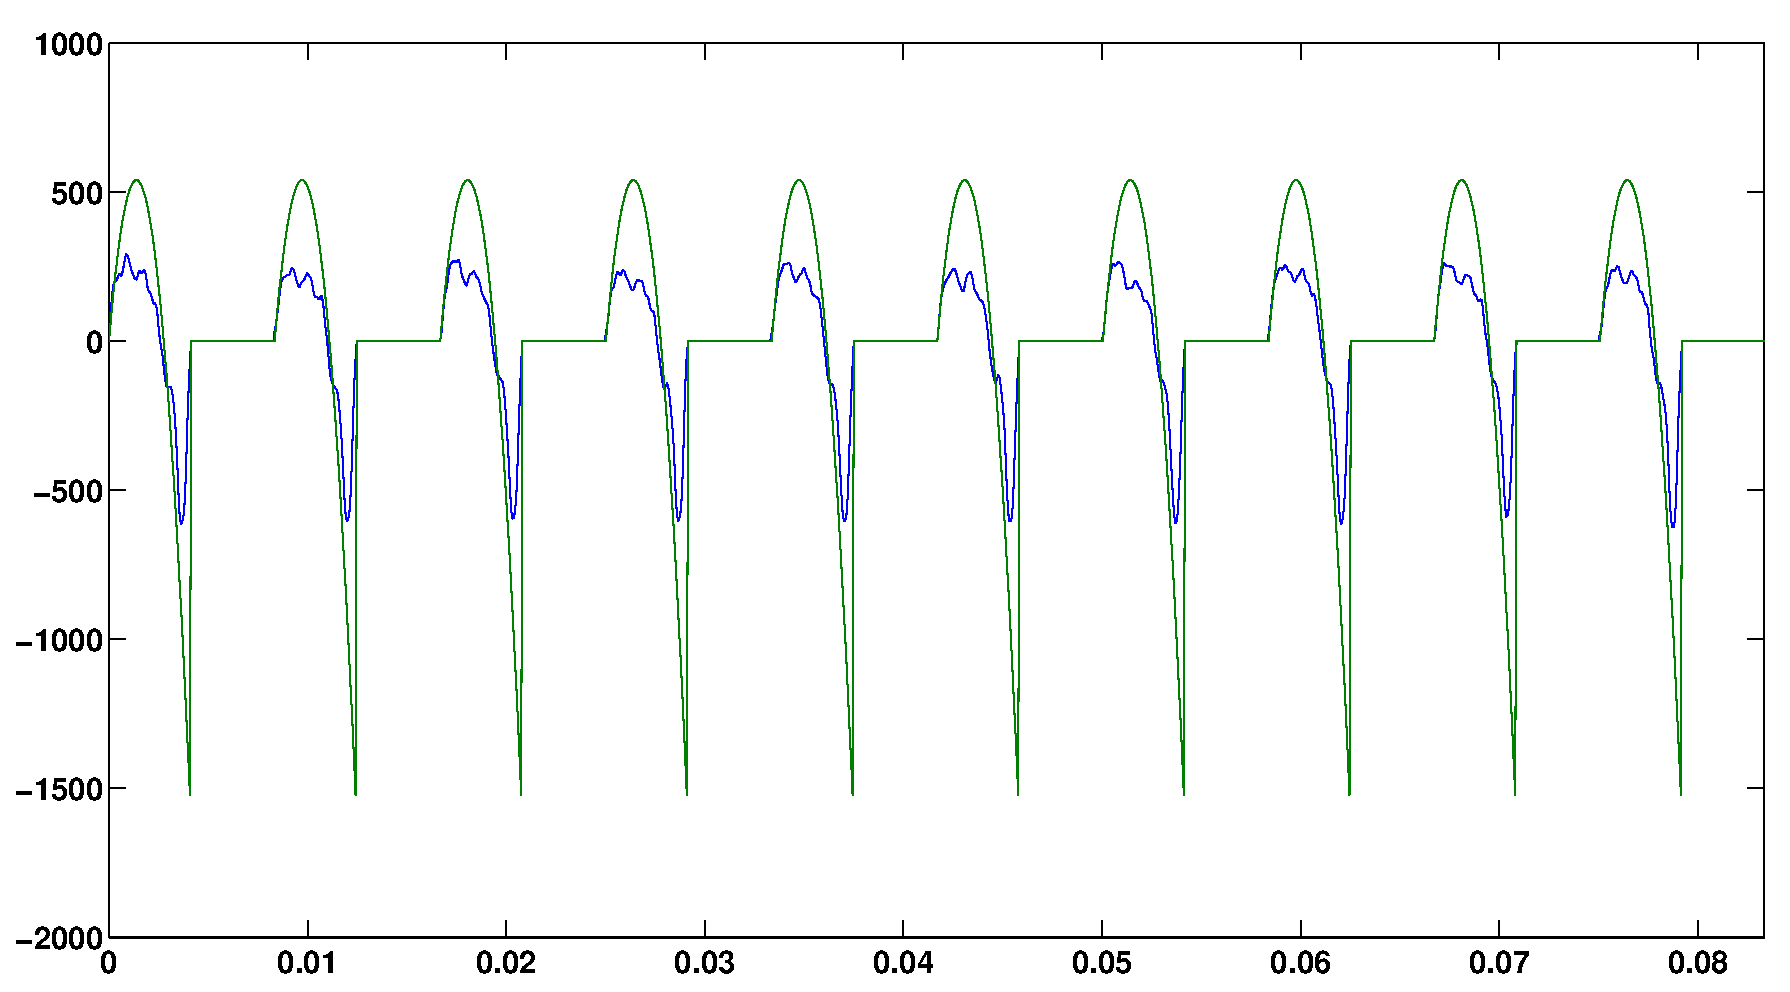
\includegraphics[scale=.3]{img/Comparison-201.eps}
\end{center}
\caption{The uppermost picture plots the relative error values vs. $\alpha$-values of the iterative calculation of the inversion. The red dot denotes the $\alpha$-value acquired from Morozov's discrepancy principle and the black dot denotes the $\alpha$-value corresponding to the least relative error in the reconstruction (from the iterative calculation). The middle picture graphs the reconstruction with the $\alpha$-value acquired from Morozov's discrepancy principle and the bottom picture graphs the reconstruction $\alpha$-value corresponding to the least relative error in the reconstruction.}
\label{fig:iter_comparison}
\end{figure}
Since the number of (a priori known) variables is quite high a large amount of data needed to be harvested in order to properly analyze the inversion method. The following figures demonstrate some of the data that was collected.
\begin{figure}[H]
\begin{center}
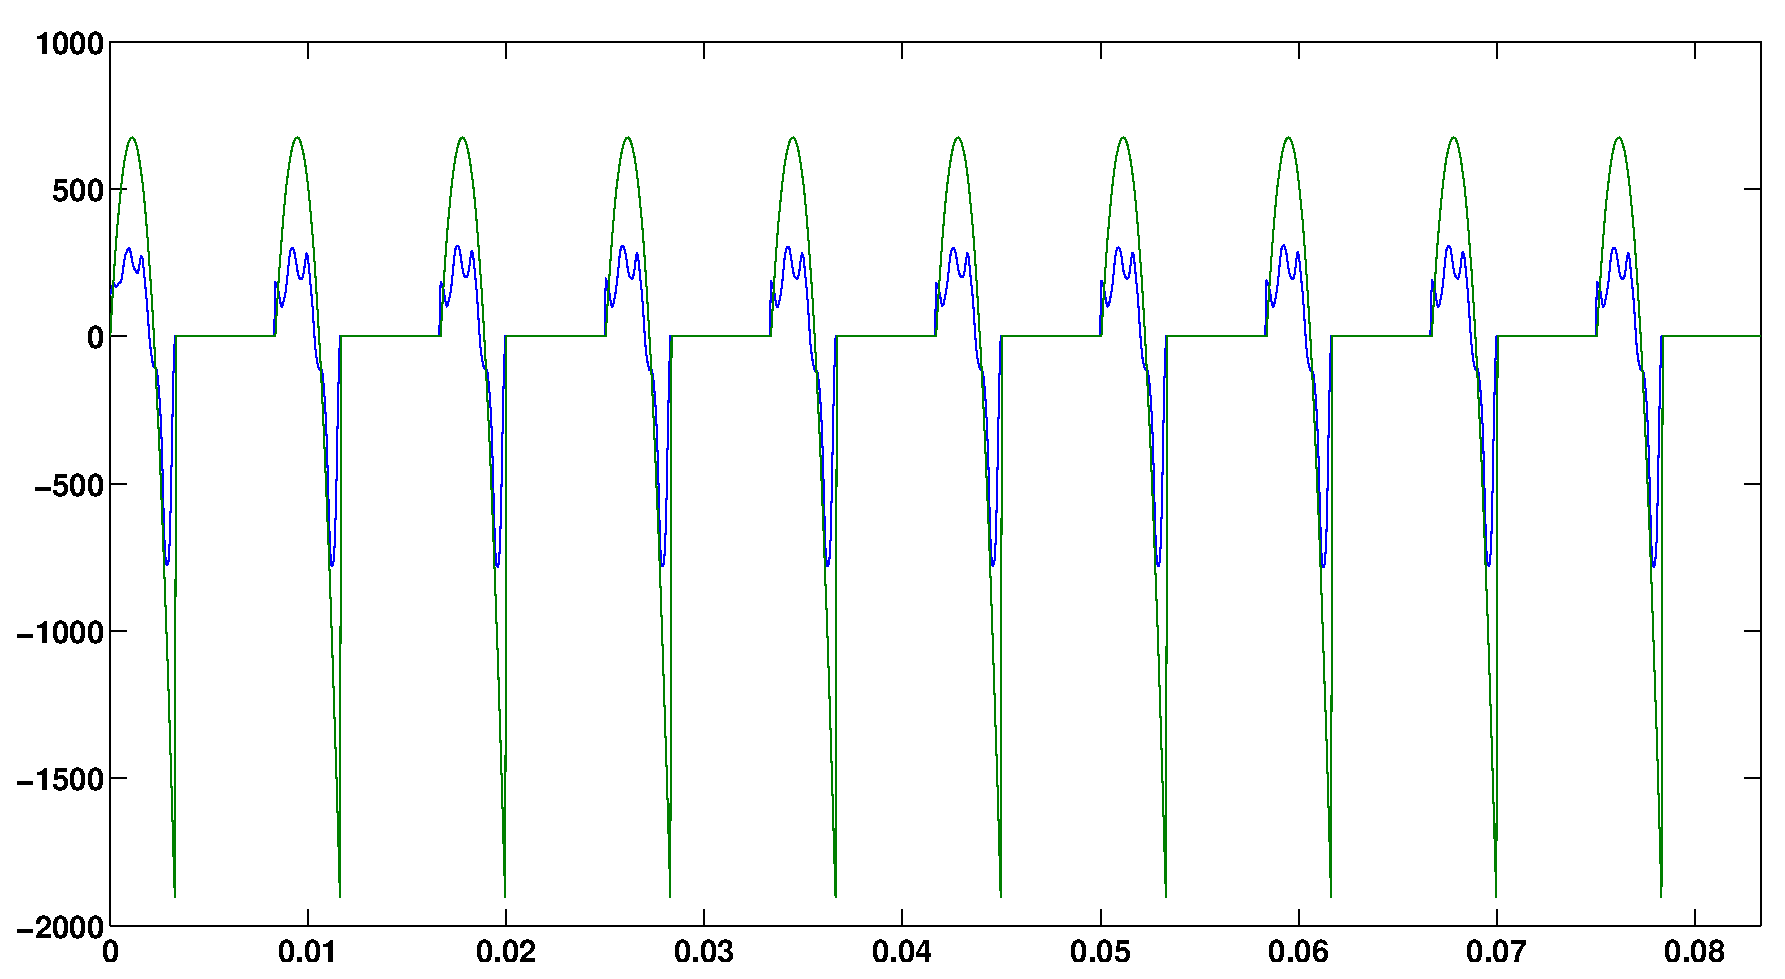
\includegraphics[scale=.3]{img/morozov_no-crime_error-005_Qrand-0.eps}
\end{center}
\caption{Sound frequency = 120 Hz, Q = 0.4, relative error of the reconstruction $\approx$ 69.1\%, $\alpha \approx 123.9$.}
\label{fig:tik-1}
\end{figure}
\begin{figure}[H]
\begin{center}
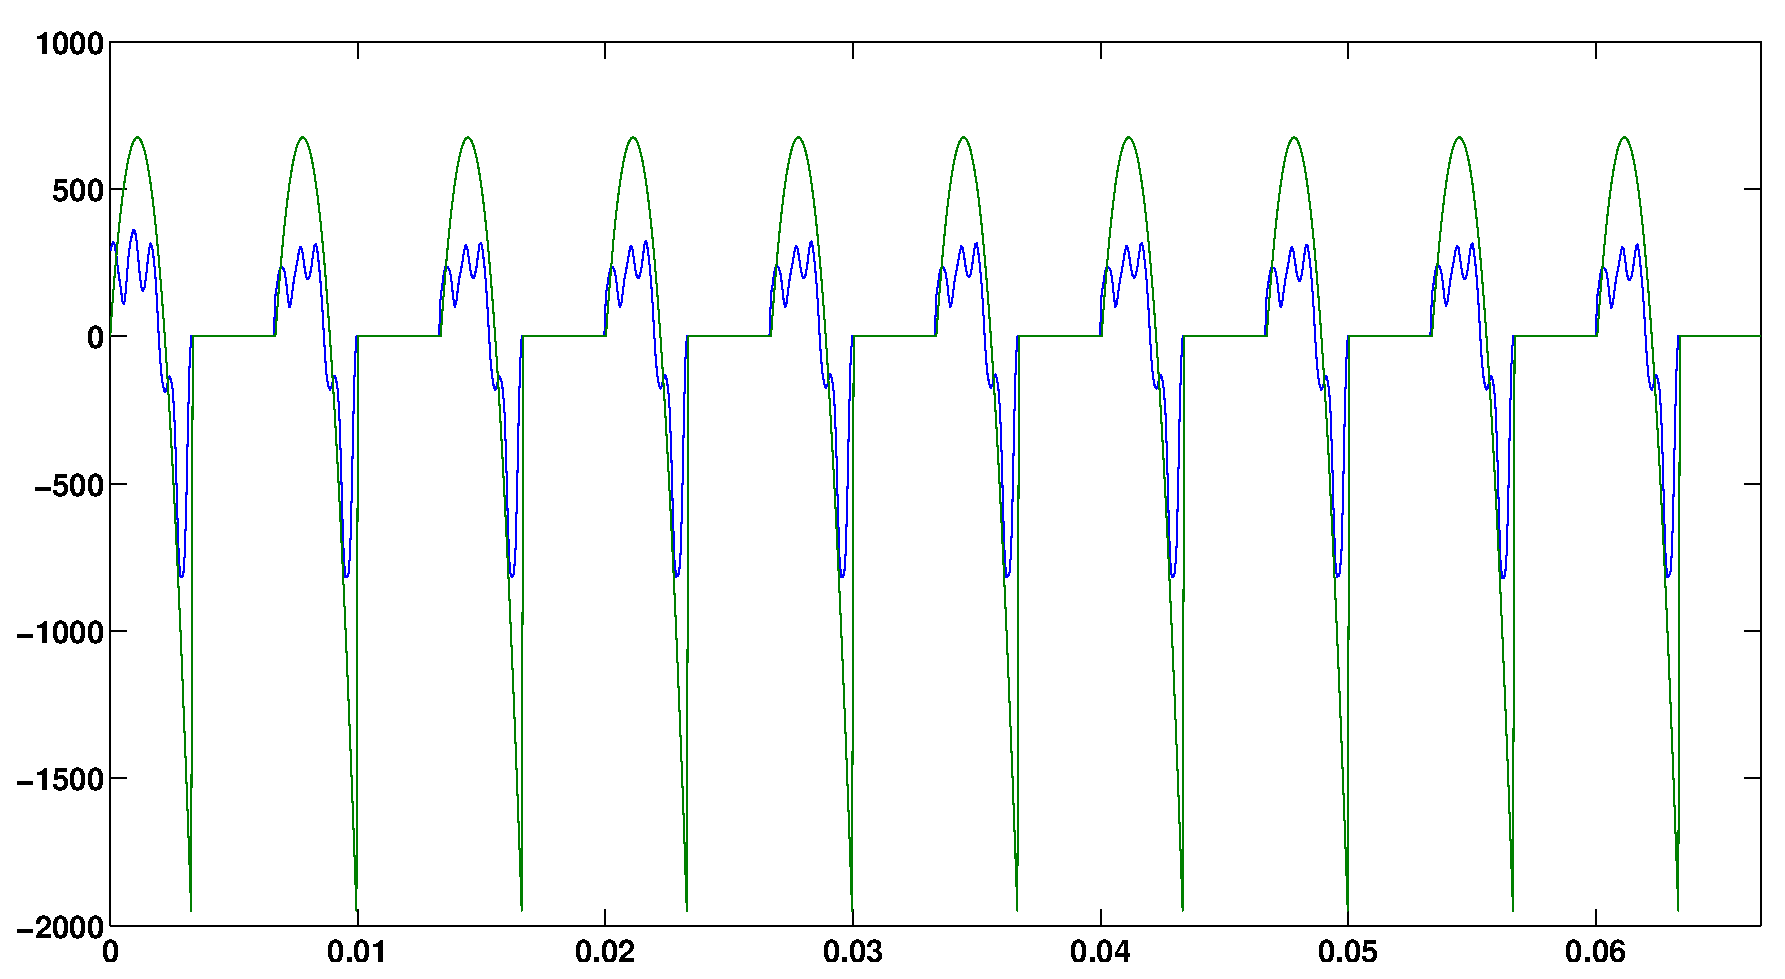
\includegraphics[scale=.3]{img/morozov_no-crime_error-005_Qrand-0[V2].eps}
\end{center}
\caption{Sound frequency = 150 Hz, Q = 0.5, relative error of the reconstruction $\approx$ 70.1\%, $\alpha \approx 86.0$.}
\label{fig:tik-2}
\end{figure}
\begin{figure}[H]
\begin{center}
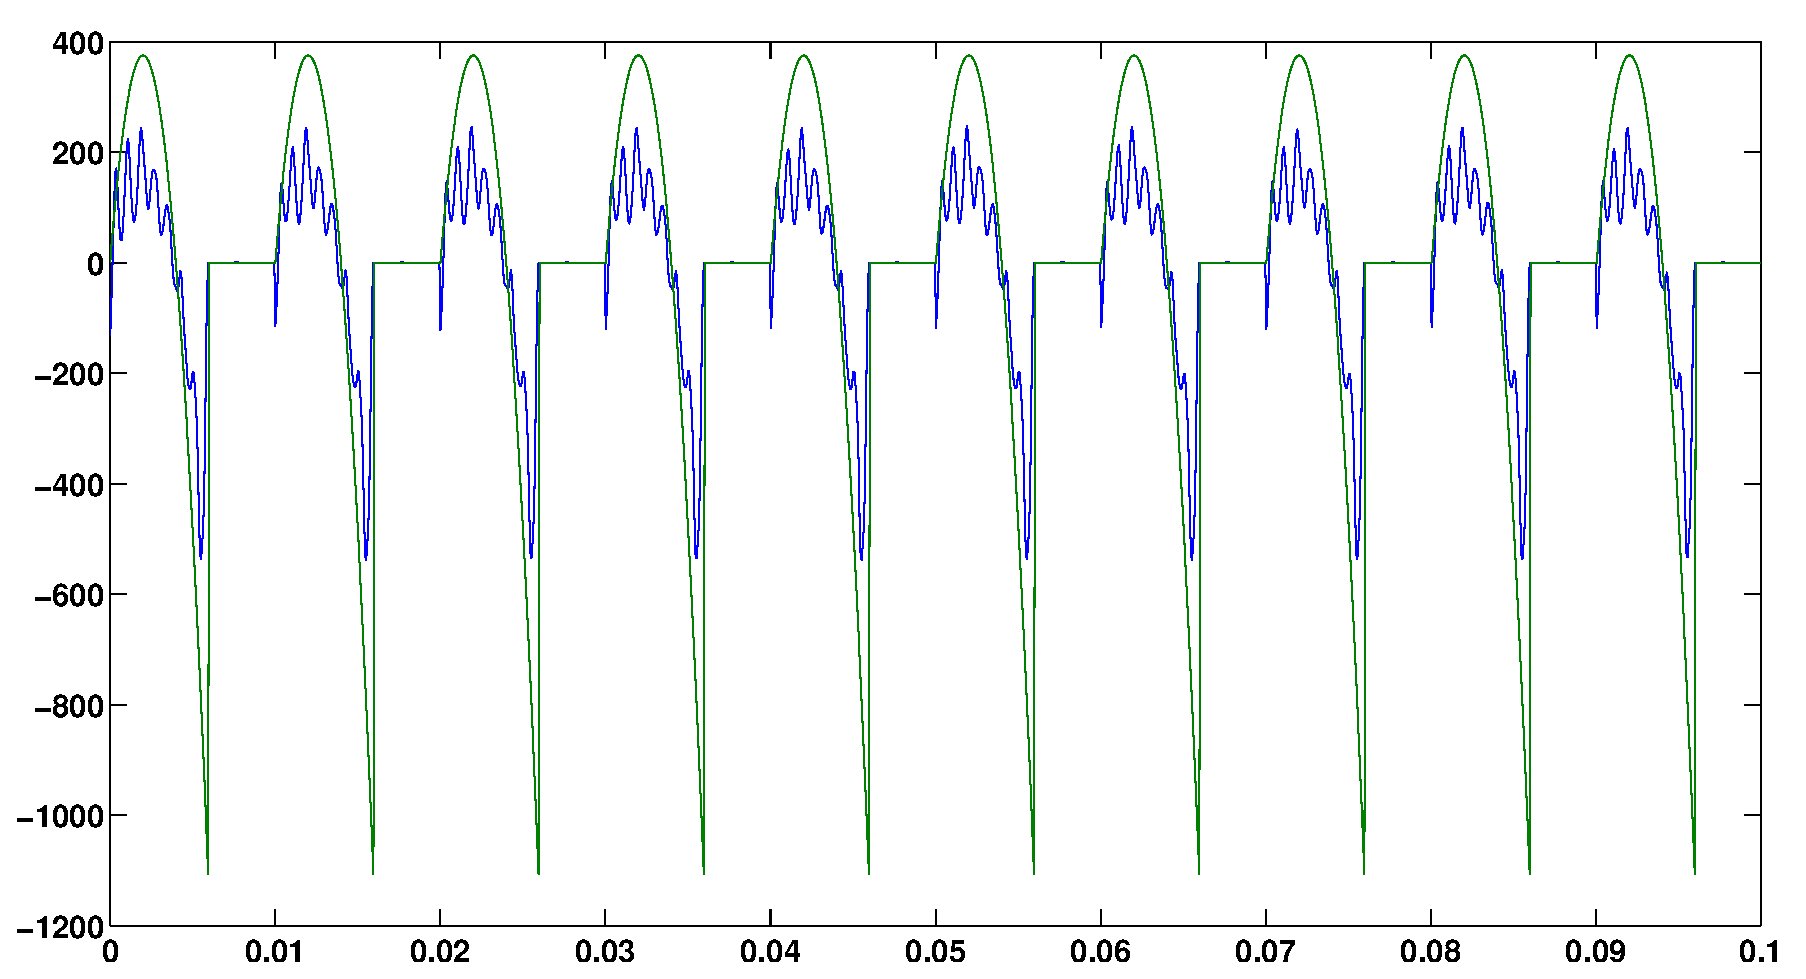
\includegraphics[scale=.3]{img/morozov_no-crime_error-005_Qrand-0[Pres].eps}
\end{center}
\caption{Sound frequency = 100 Hz, Q = 0.6, relative error of the reconstruction $\approx$ 64.1\%, $\alpha \approx 66.6$.}
\label{fig:tik-3}
\end{figure}
\begin{figure}[H]
\begin{center}
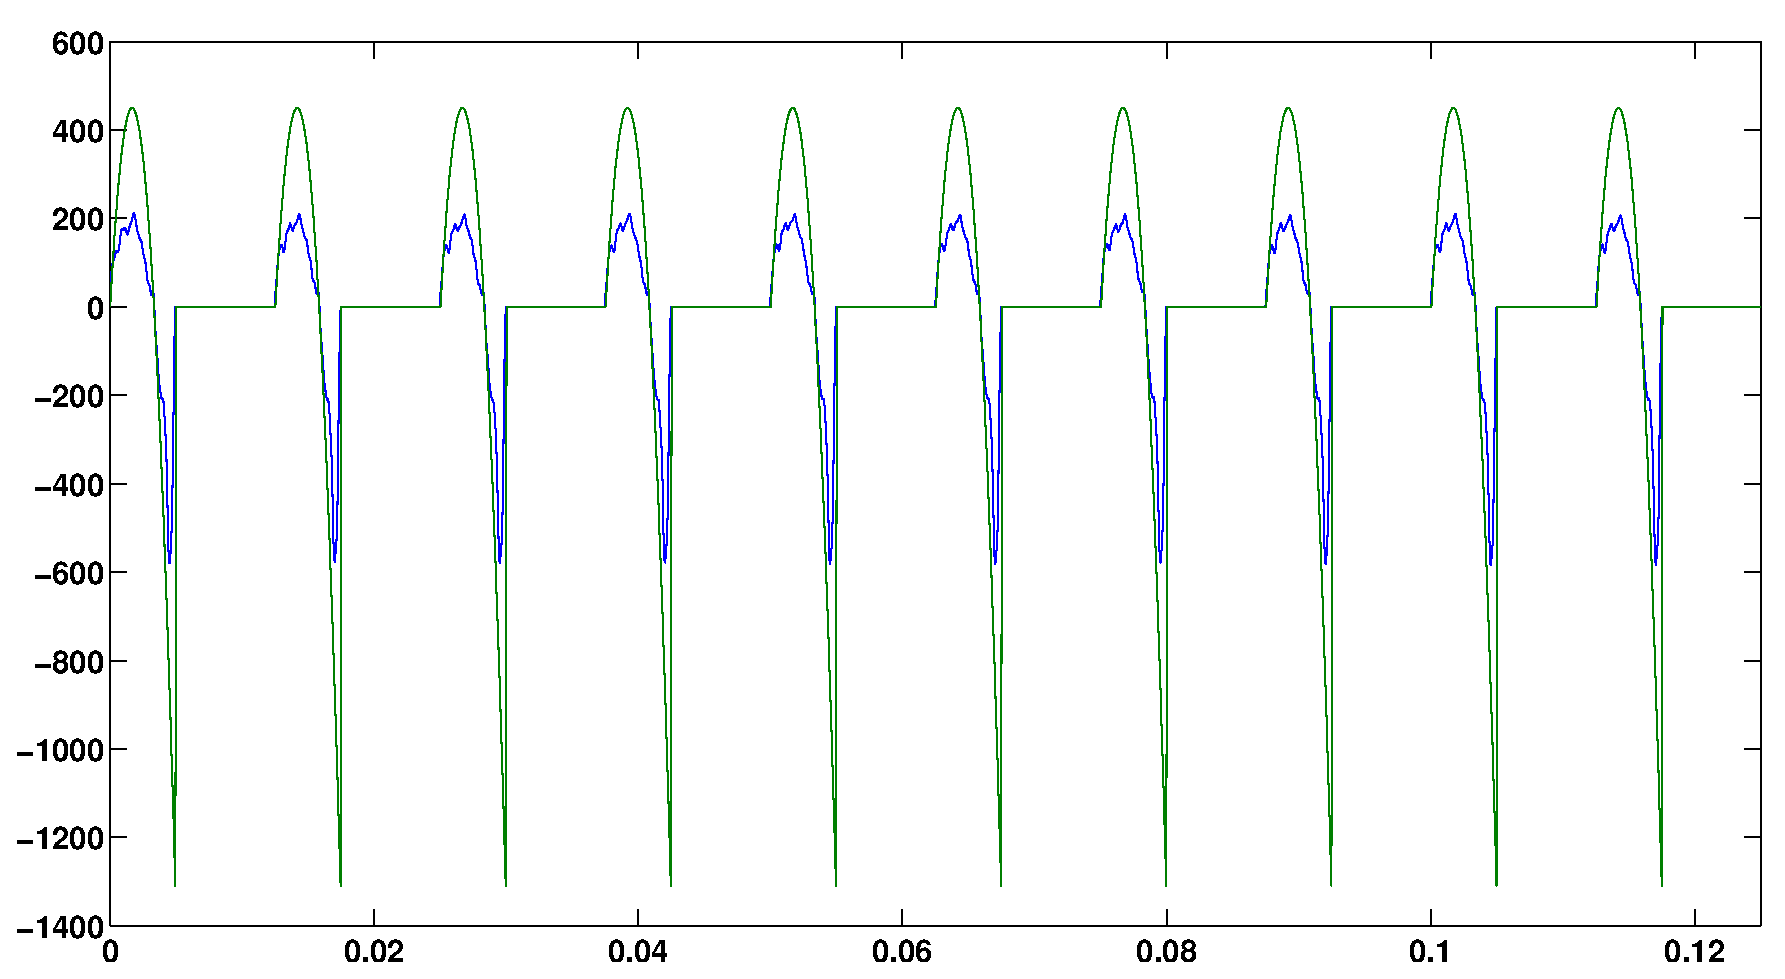
\includegraphics[scale=.3]{img/morozov_no-crime_error-005_Qrand-0[Pres-V4].eps}
\end{center}
\caption{Sound frequency = 80 Hz, Q = 0.3, relative error of the reconstruction $\approx$ 64.6\%, $\alpha \approx 84.5$.}
\label{fig:tik-4}
\end{figure}
\begin{figure}[H]
\begin{center}
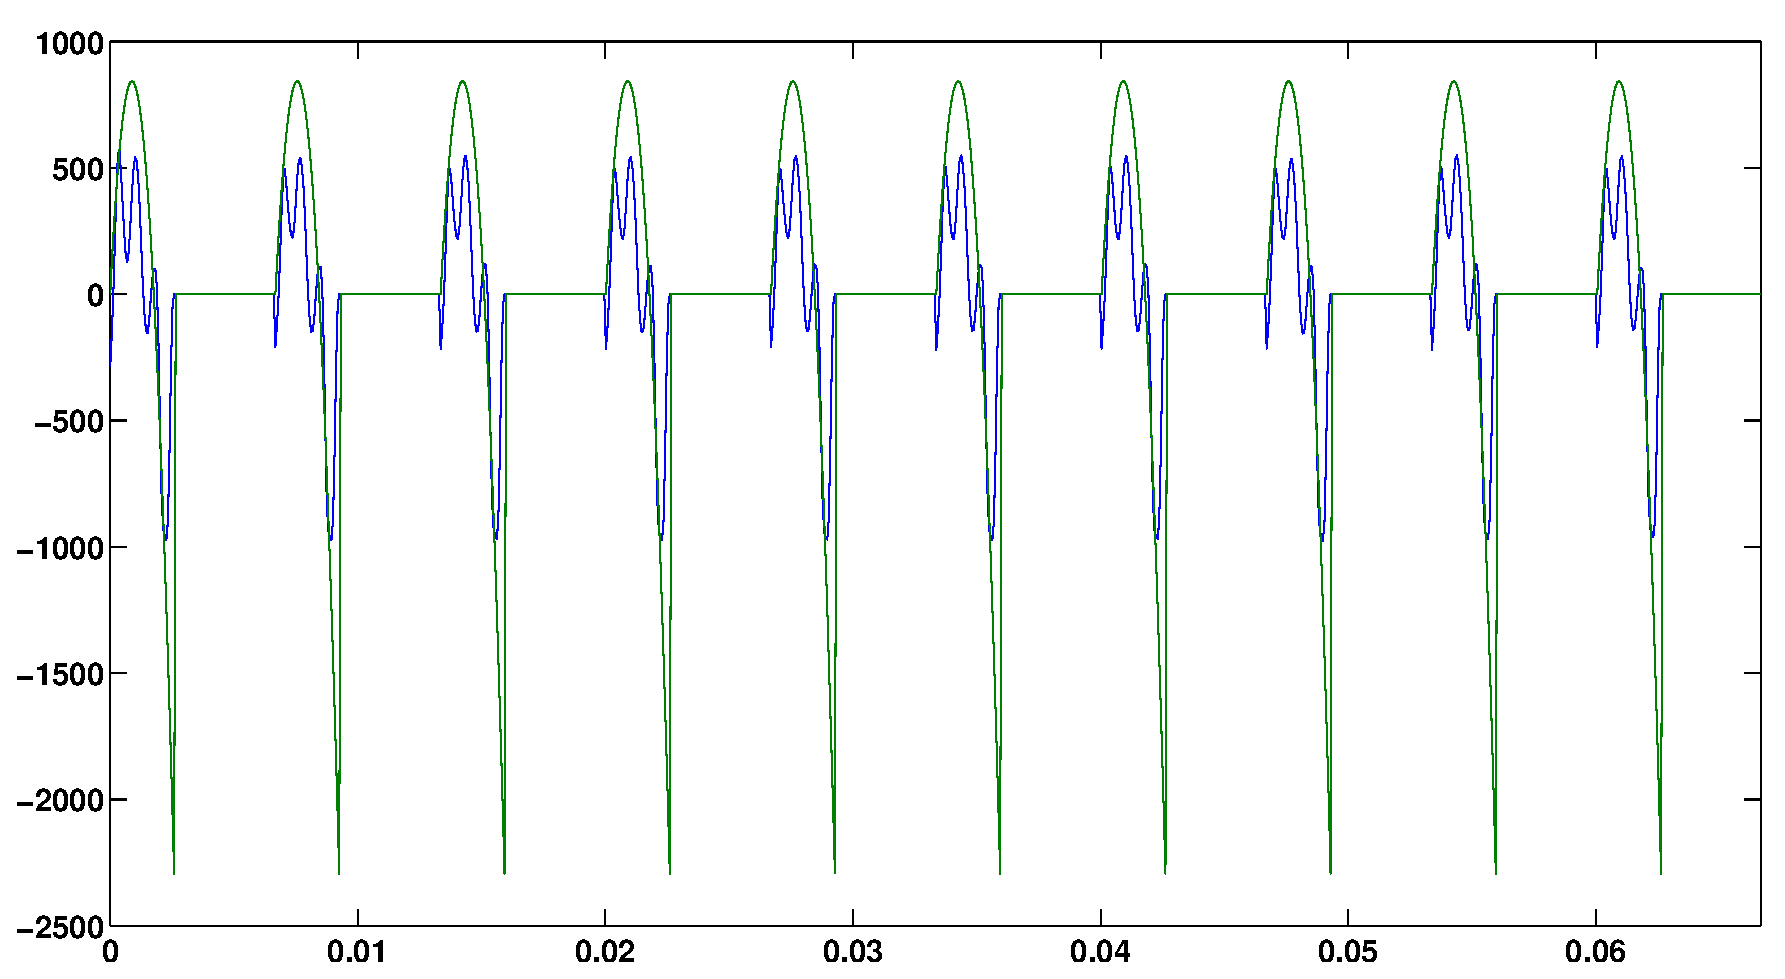
\includegraphics[scale=.3]{img/morozov_no-crime_error-005_Qrand-0[Pres-V2].eps}
\end{center}
\caption{Sound frequency = 150 Hz, Q = 0.4, relative error of the reconstruction $\approx$ 74.0\%, $\alpha \approx 48.5$.}
\label{fig:tik-5}
\end{figure}

\subsection{Results of the approximation method for \\approximating the Klatt-parameter}
\label{sec:KlattApprox}

In this section we will present results obtained during the approximation of the Klatt-parameter (algorithm previously described in section \ref{sec:approxKlatt}). We will present the results as
\begin{itemize}
 \item plots of four periods of both the target and reconstructed glottal excitation signal
 \item plots of only one period of the reconstructed glottal excitation signal.
\end{itemize}
The $Q_{guess}$ parameter acquired from the algorithm is visualized as a black dot in the plots mentioned above (anchored to the x-axis). The approximation routine was applied on both synthetic and actual data. \newpage

\begin{figure}[H]
\begin{center}
 \caption*{In figures \ref{fig:app1-beginning} to \ref{fig:app1-end} the signal frequency is 120 Hz. The approximation algorithm acquired $Q_{guess} = 0.165$ at the end of the iterations, while the actual parameter $Q = 0.15$, relative error of the reconstruction $\approx$ 64.6\%, $\alpha \approx 84.5$. }
 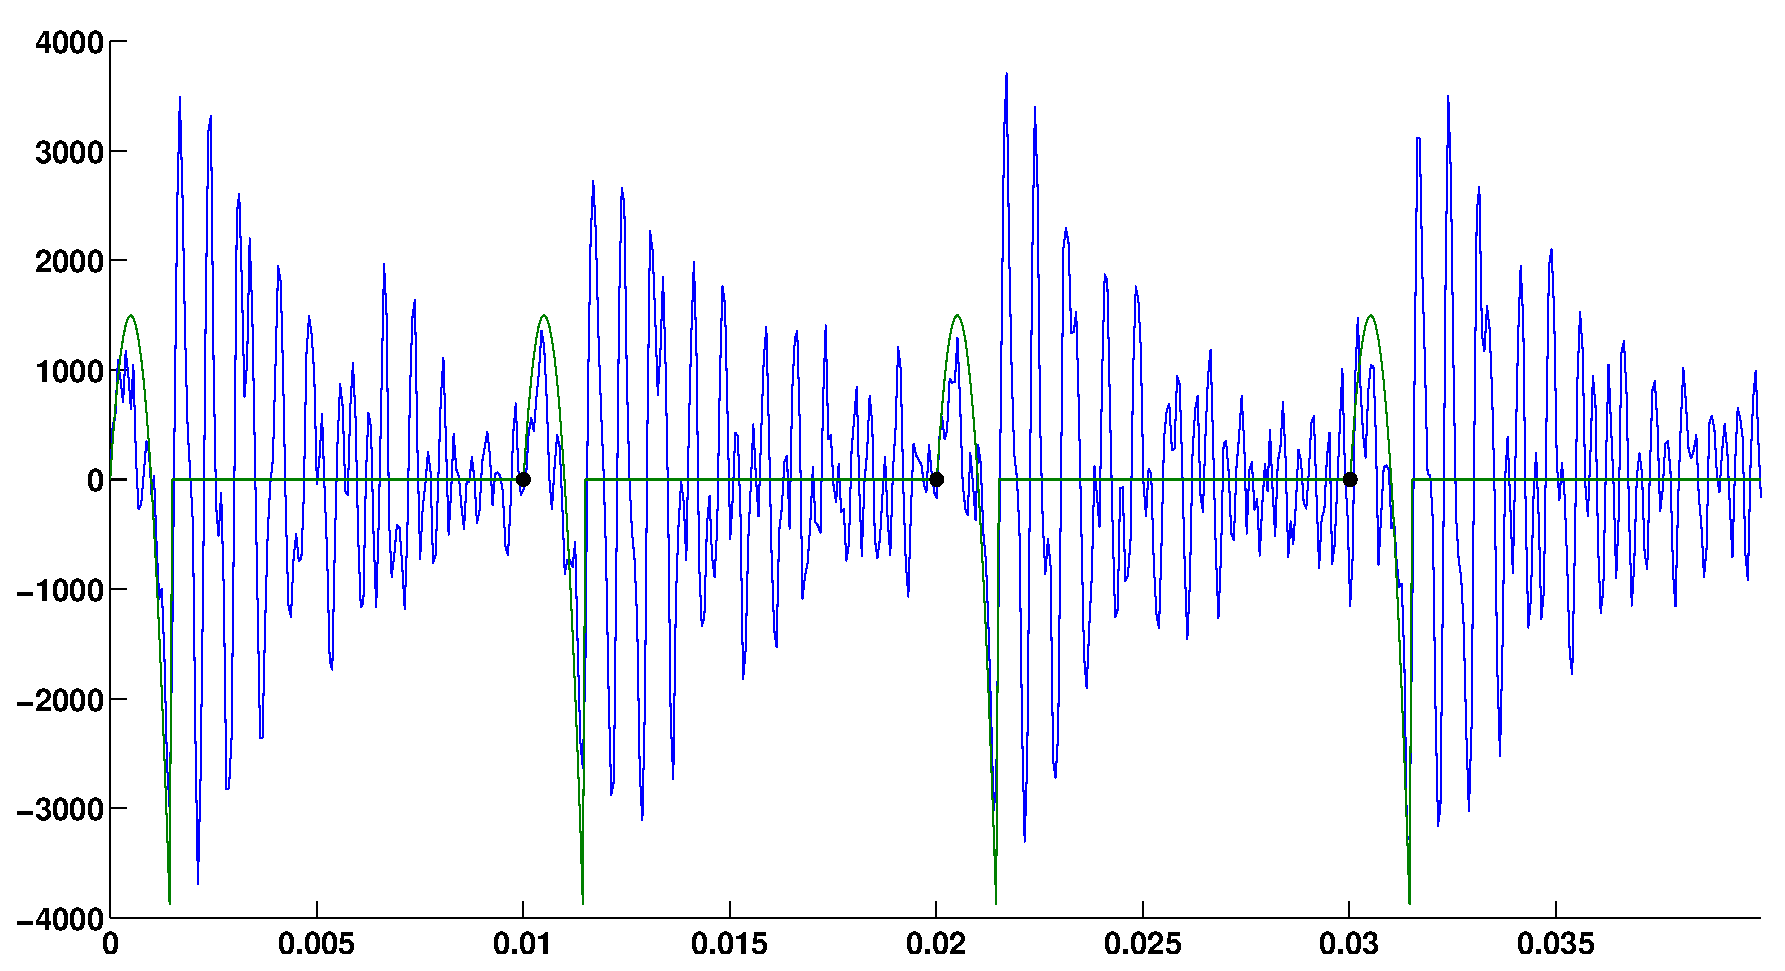
\includegraphics[scale=.3]{img/Approx_iter_wRef-v2-1.eps}
 \caption{Iteration no. 1}\label{fig:app1-beginning}
 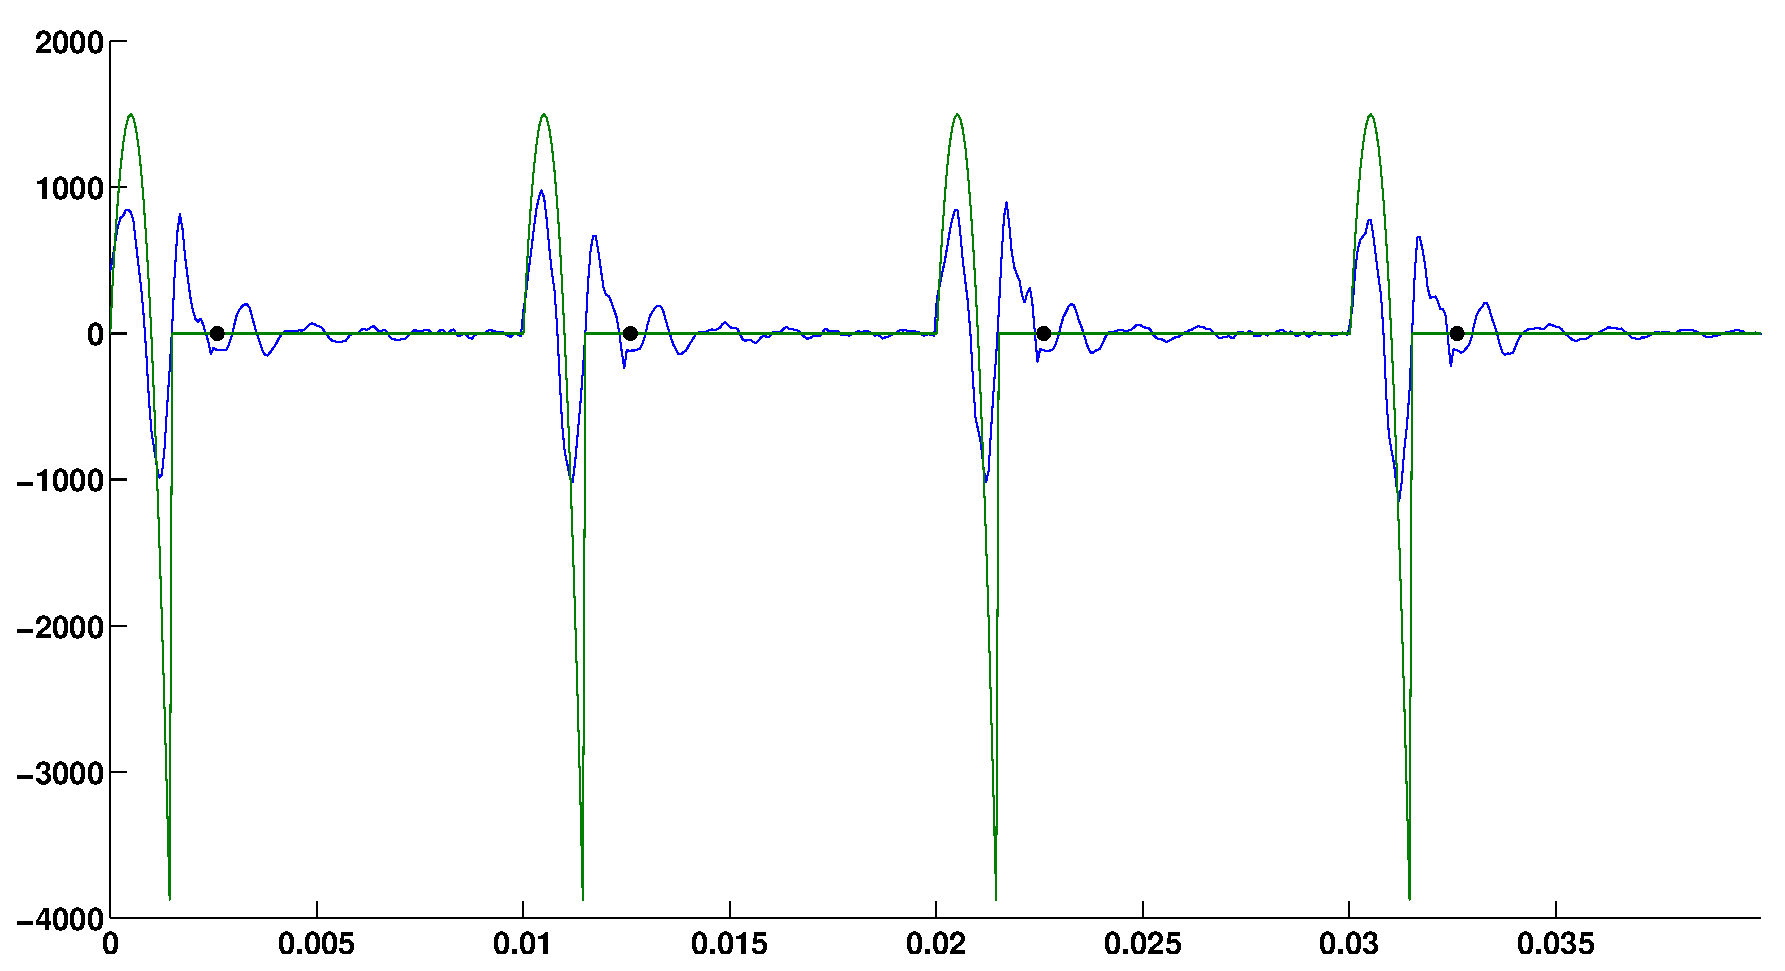
\includegraphics[scale=.3]{img/Approx_iter_wRef-v2-2.eps}
 \caption{Iteration no. 2}
 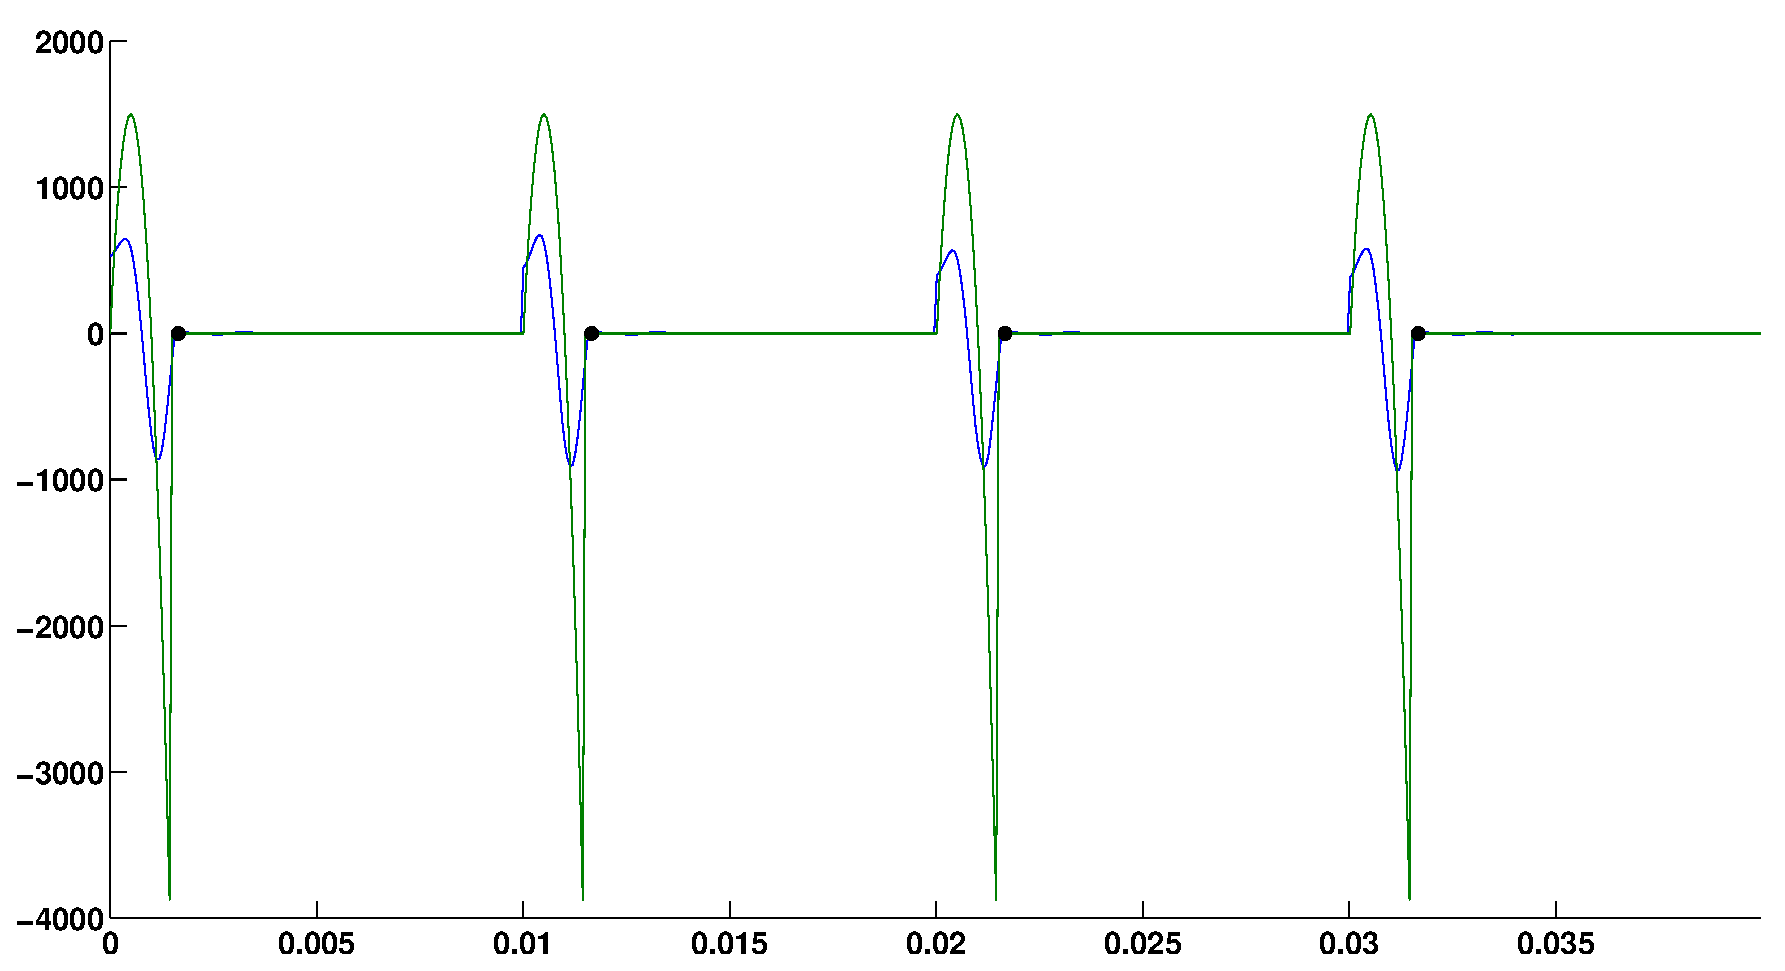
\includegraphics[scale=.3]{img/Approx_iter_wRef-v2-4.eps}
 \caption{Iteration no. 5.}
\end{center}
\end{figure}

\begin{figure}[H]
\begin{center}
 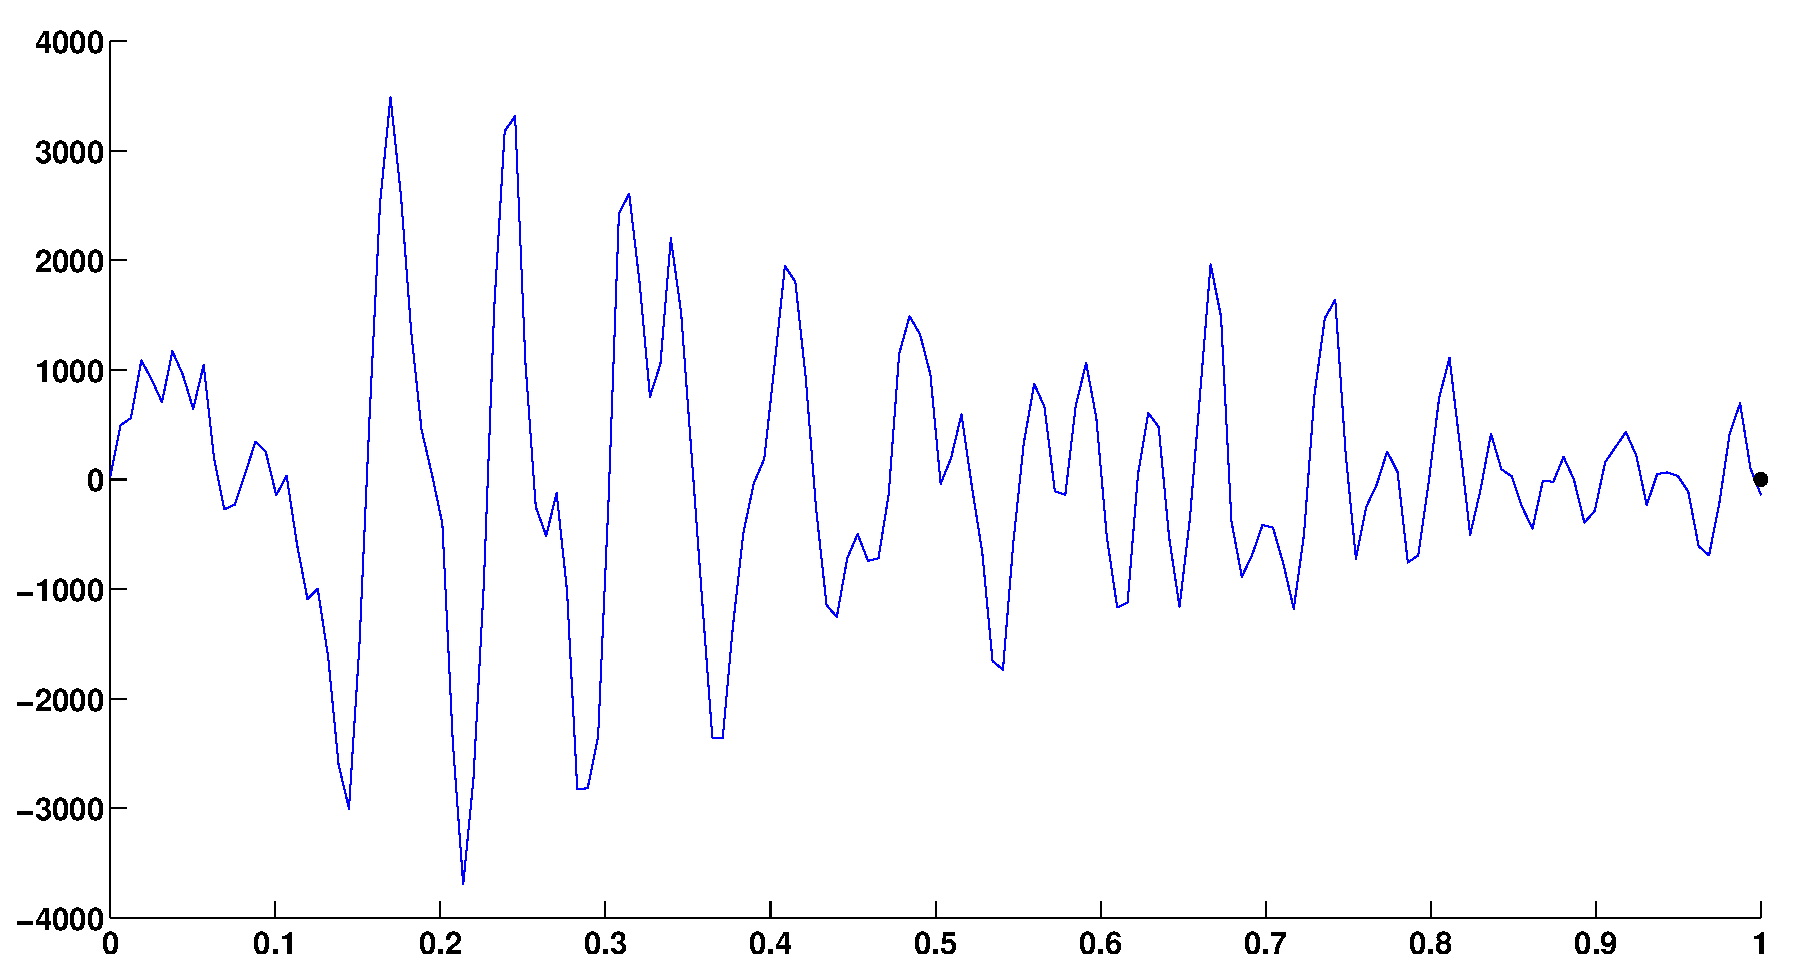
\includegraphics[scale=.35]{img/Approx_iter_onePer-v2-1.eps}
 \caption{Iteration no. 1}
 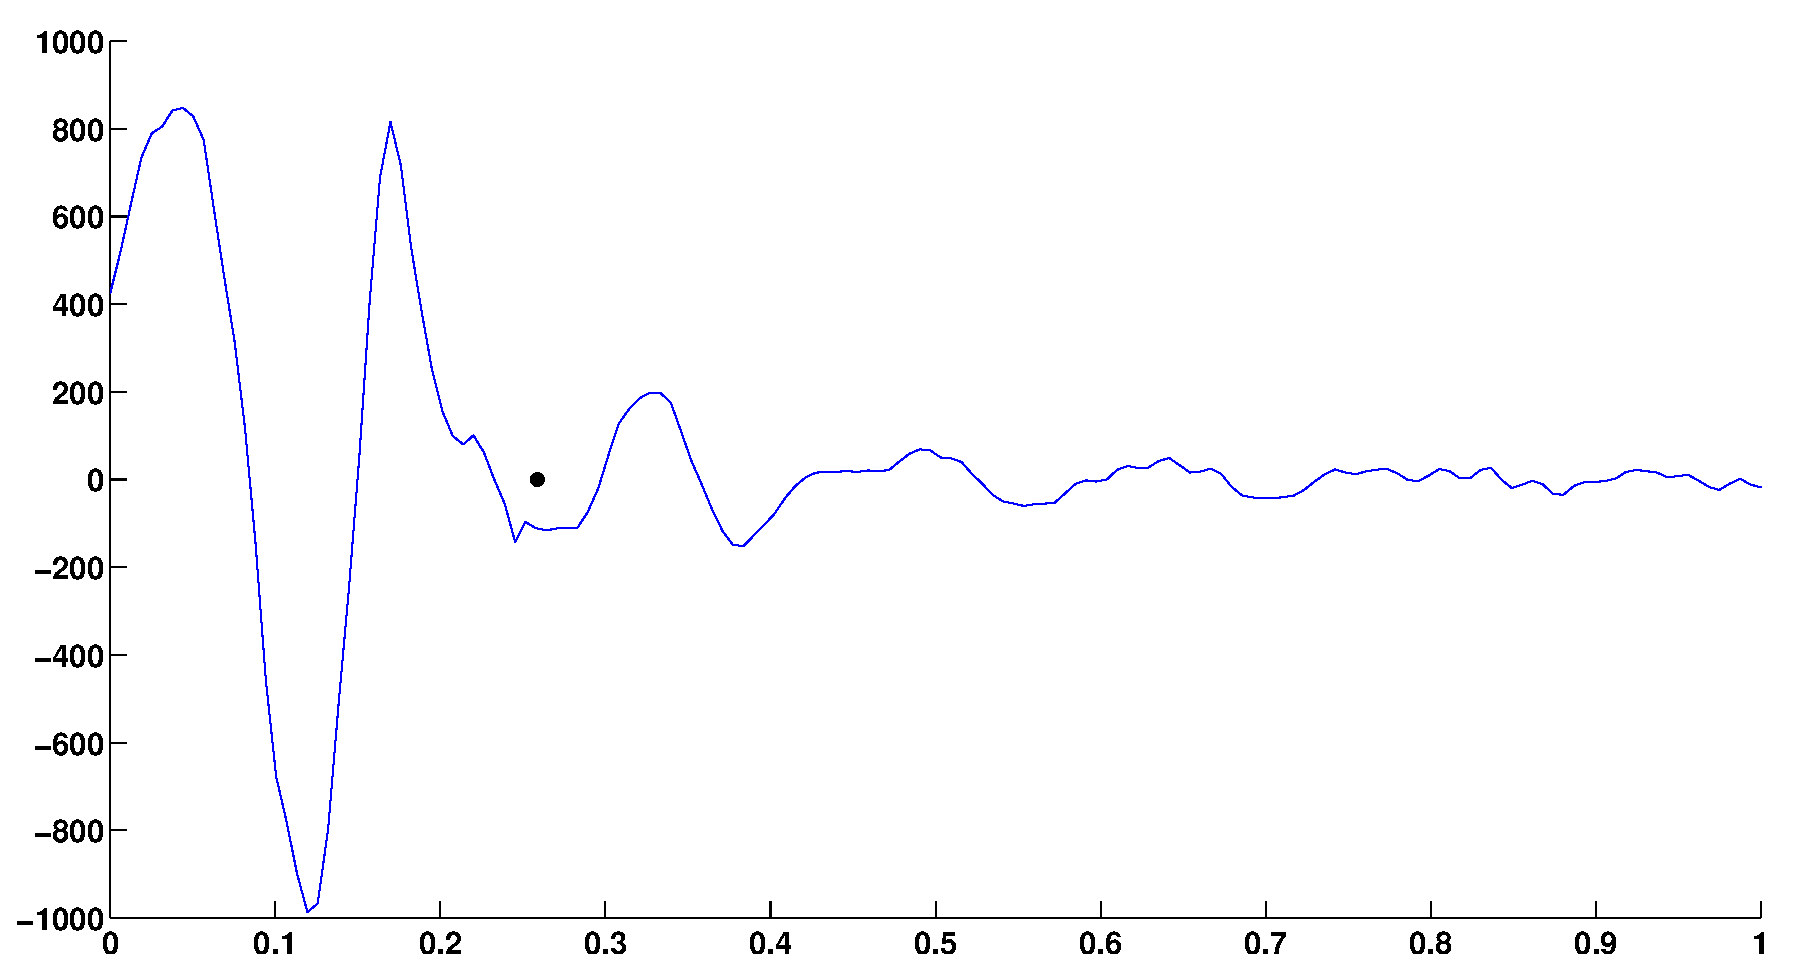
\includegraphics[scale=.35]{img/Approx_iter_onePer-v2-2.eps}
 \caption{Iteration no. 2}
 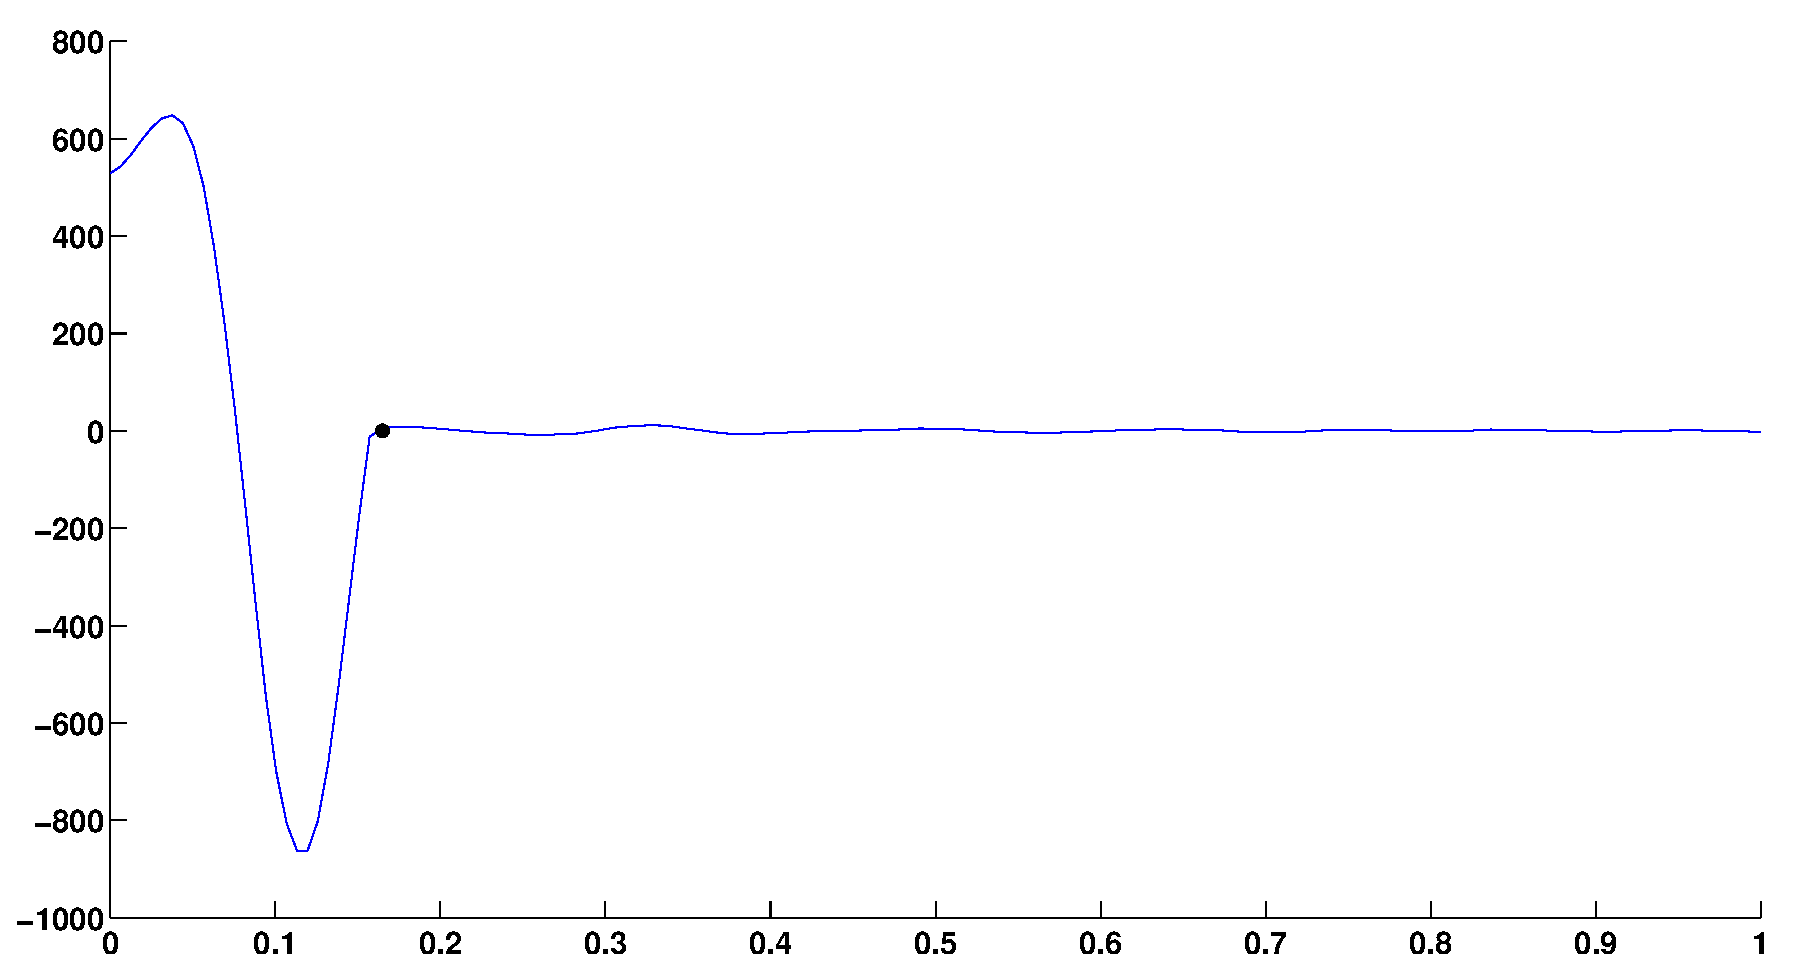
\includegraphics[scale=.35]{img/Approx_iter_onePer-v2-4.eps}
 \caption{Iteration no. 5}\label{fig:app1-end}
\end{center}
\end{figure}


\begin{figure}[H]
\begin{center}
 \caption*{In figures \ref{fig:app2-beginning} to \ref{fig:app2-end} the signal frequency is 123 Hz. The approximation algorithm acquired $Q_{guess} = 0.391$ at the end of the iterations, while the actual parameter $Q = 0.4$, relative error of the reconstruction $\approx$ 72.7\%, $\alpha \approx 167.5$. }
 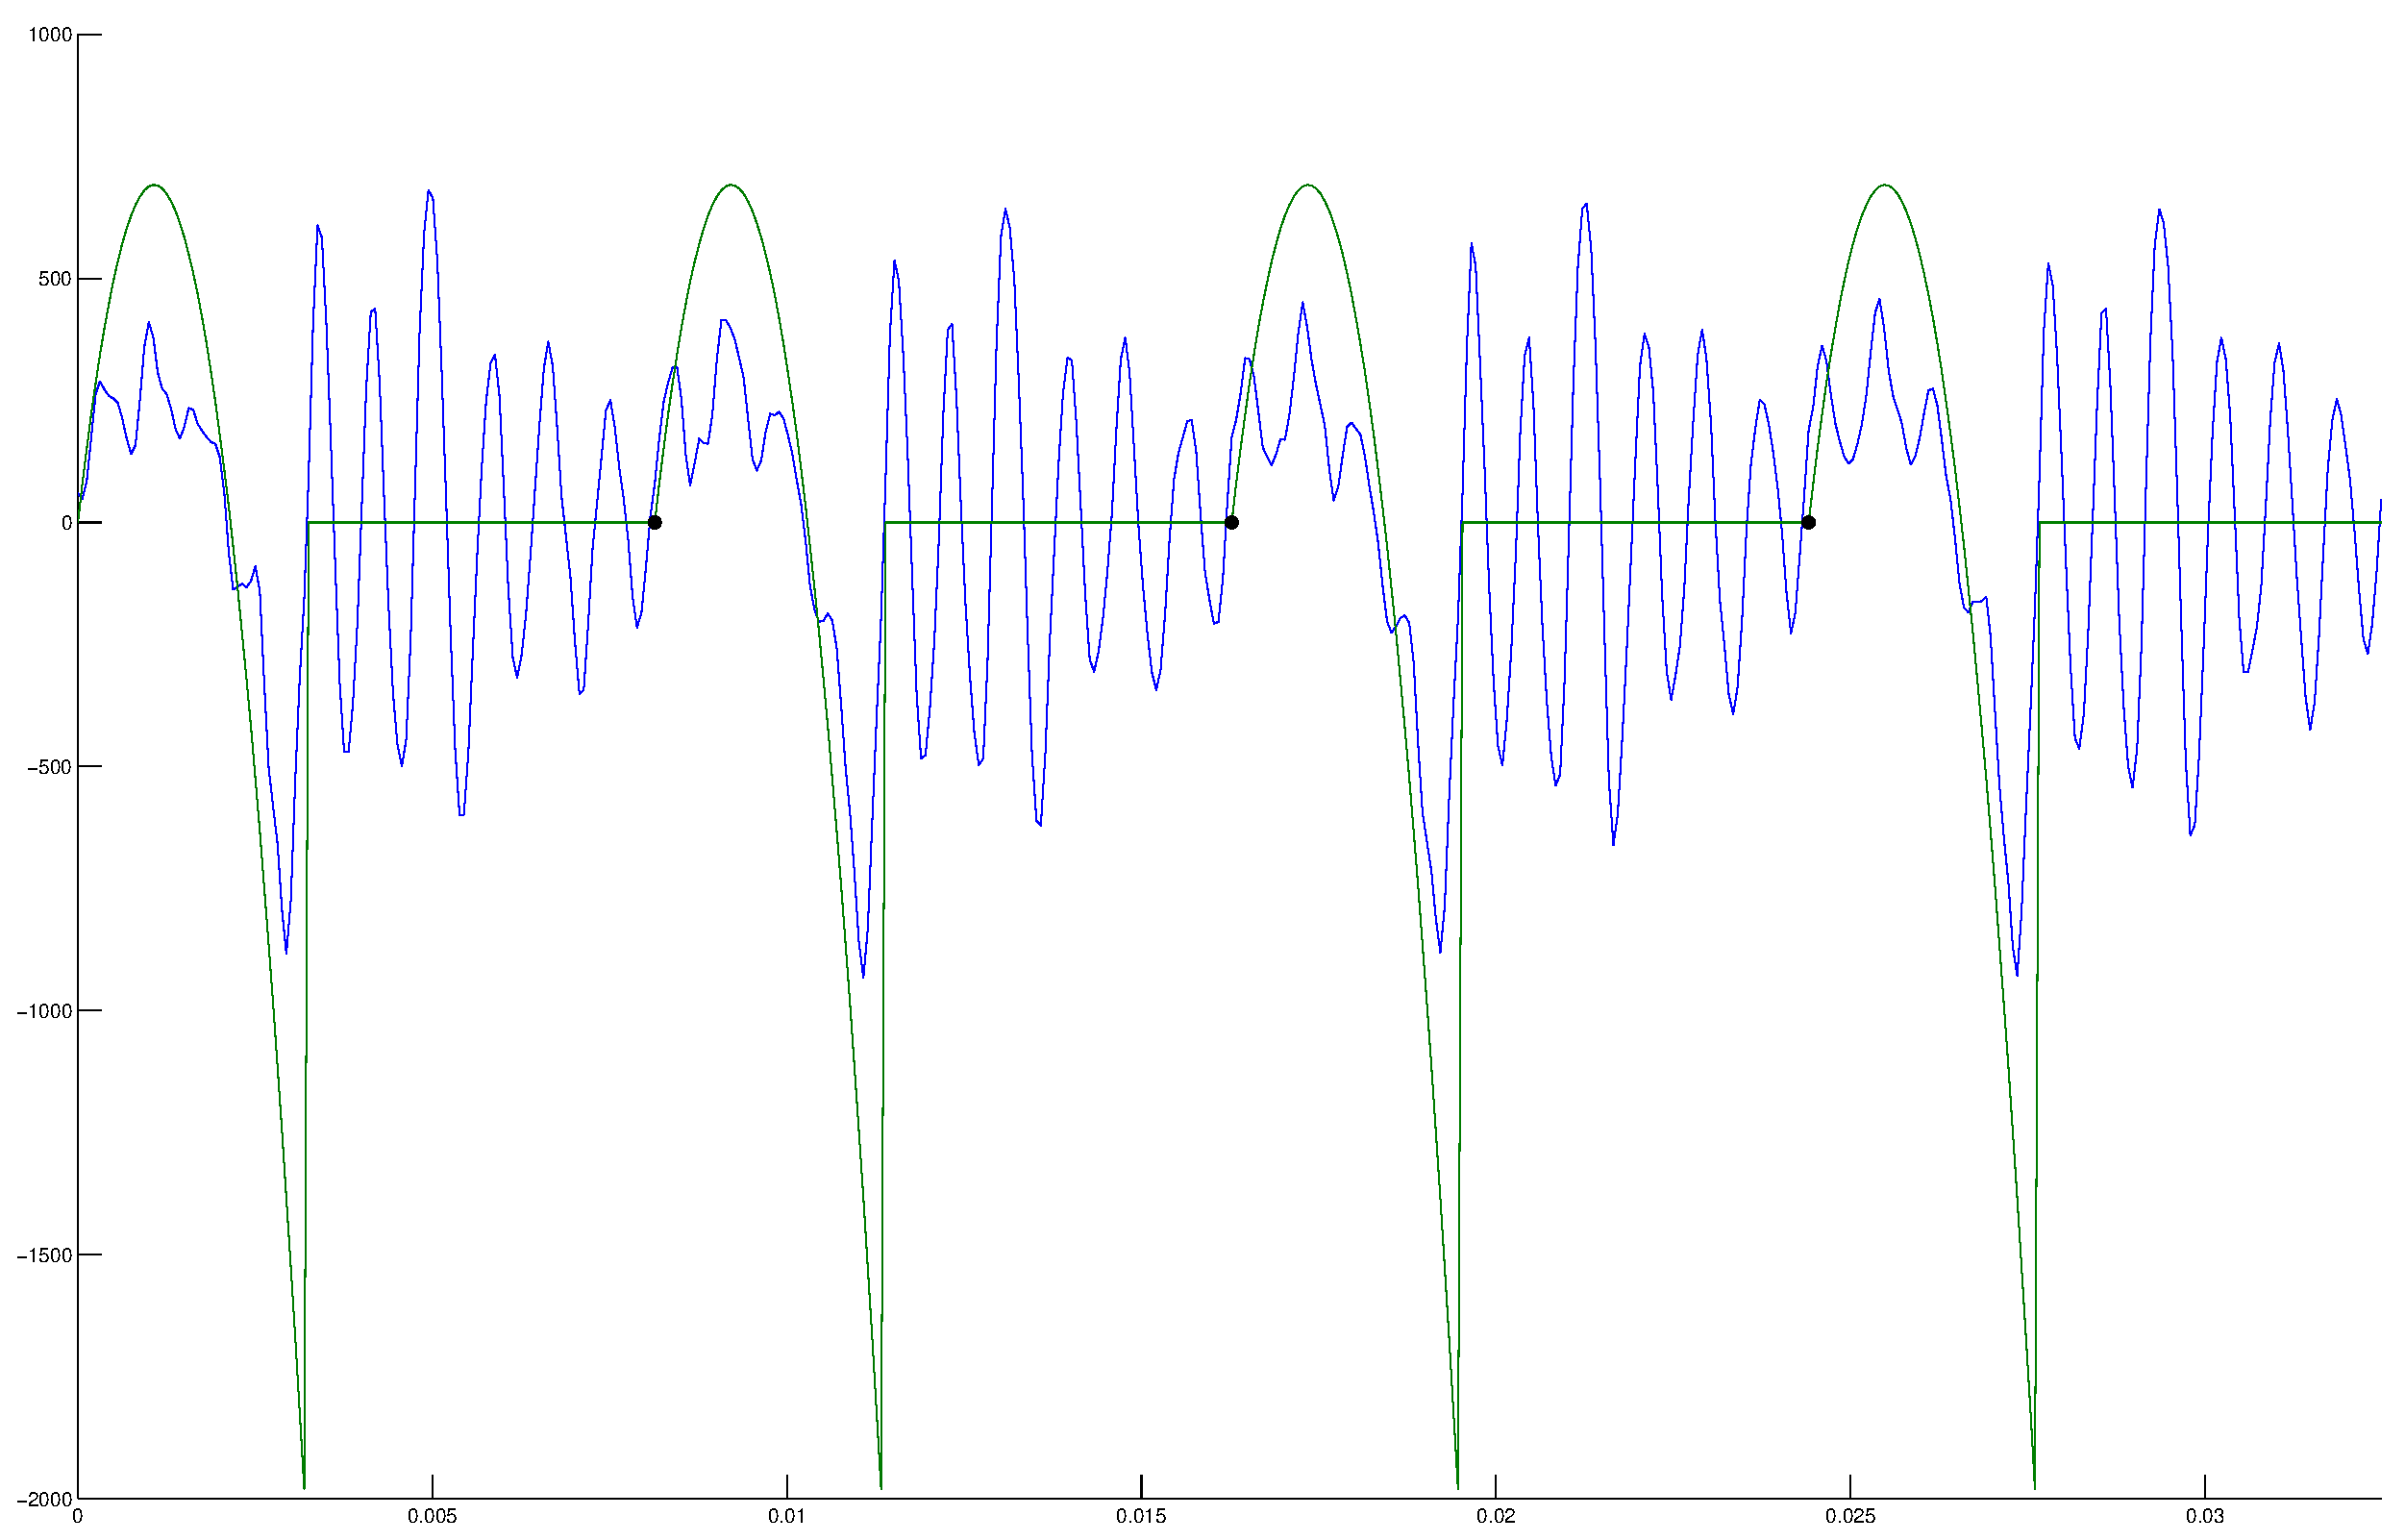
\includegraphics[scale=.2]{img/Approx_iter_wRef-1.eps}
 \caption{Iteration no.1}\label{fig:app2-beginning}
 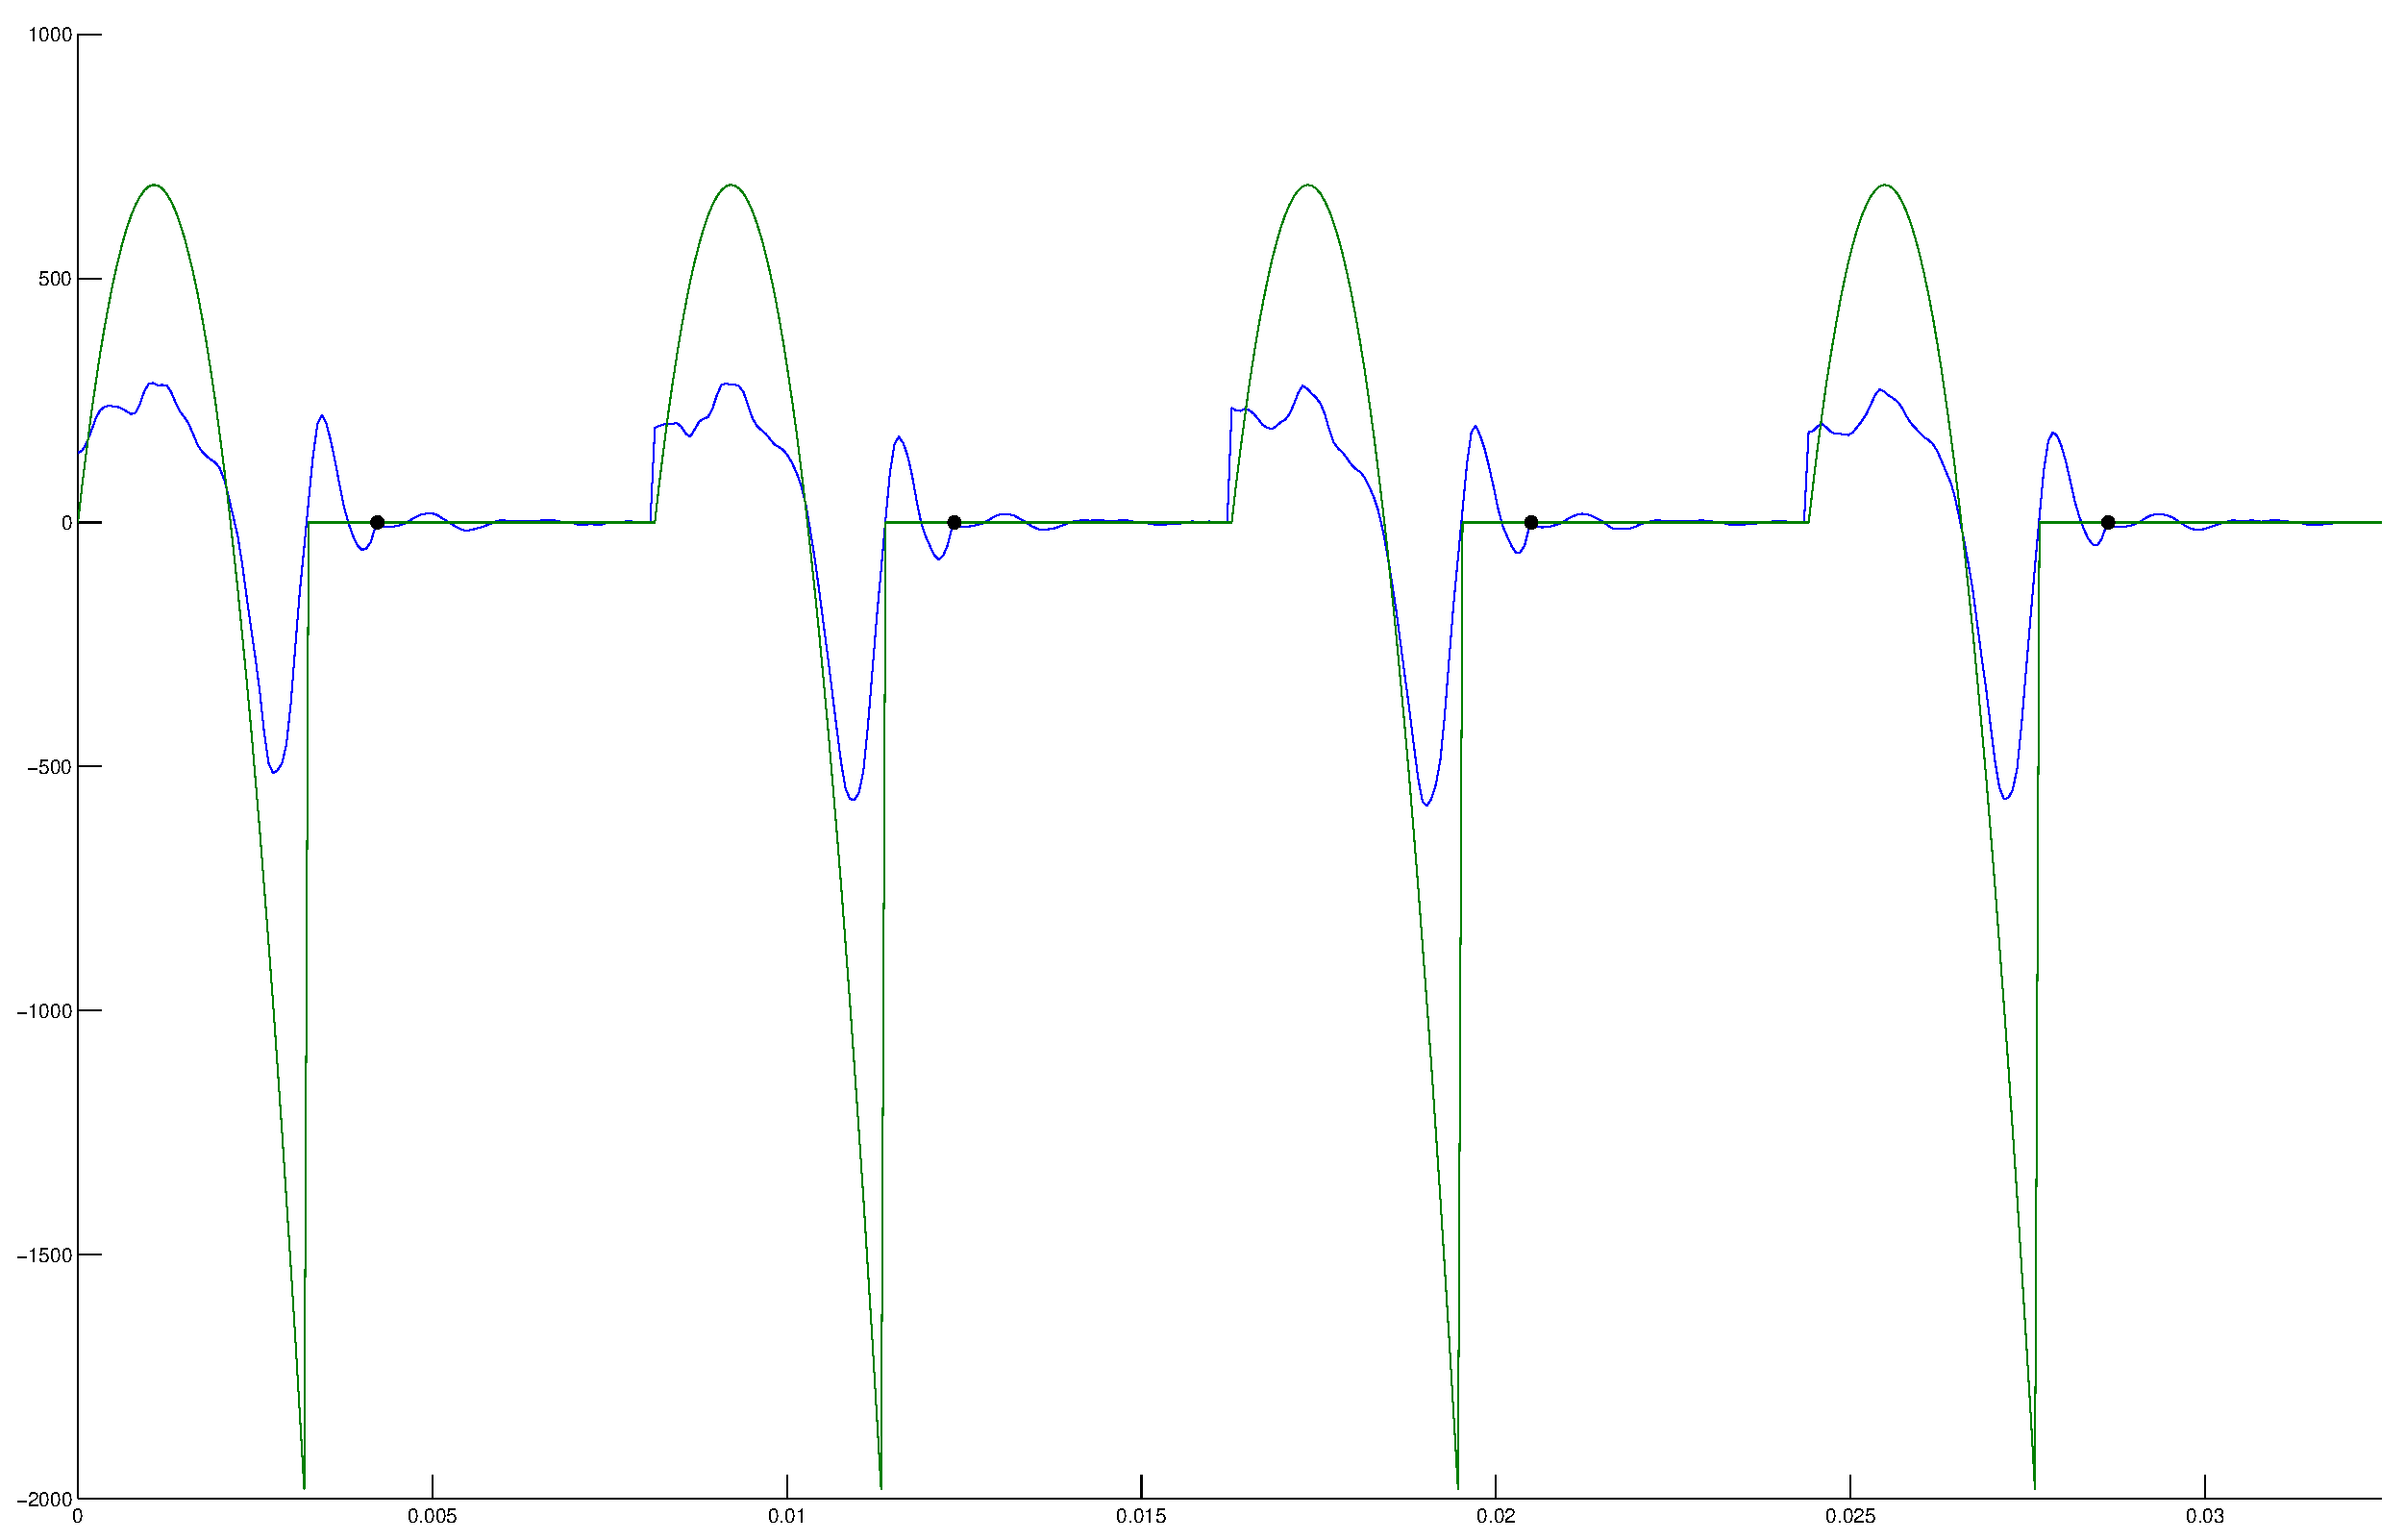
\includegraphics[scale=.2]{img/Approx_iter_wRef-2.eps}
 \caption{Iteration no.2}
 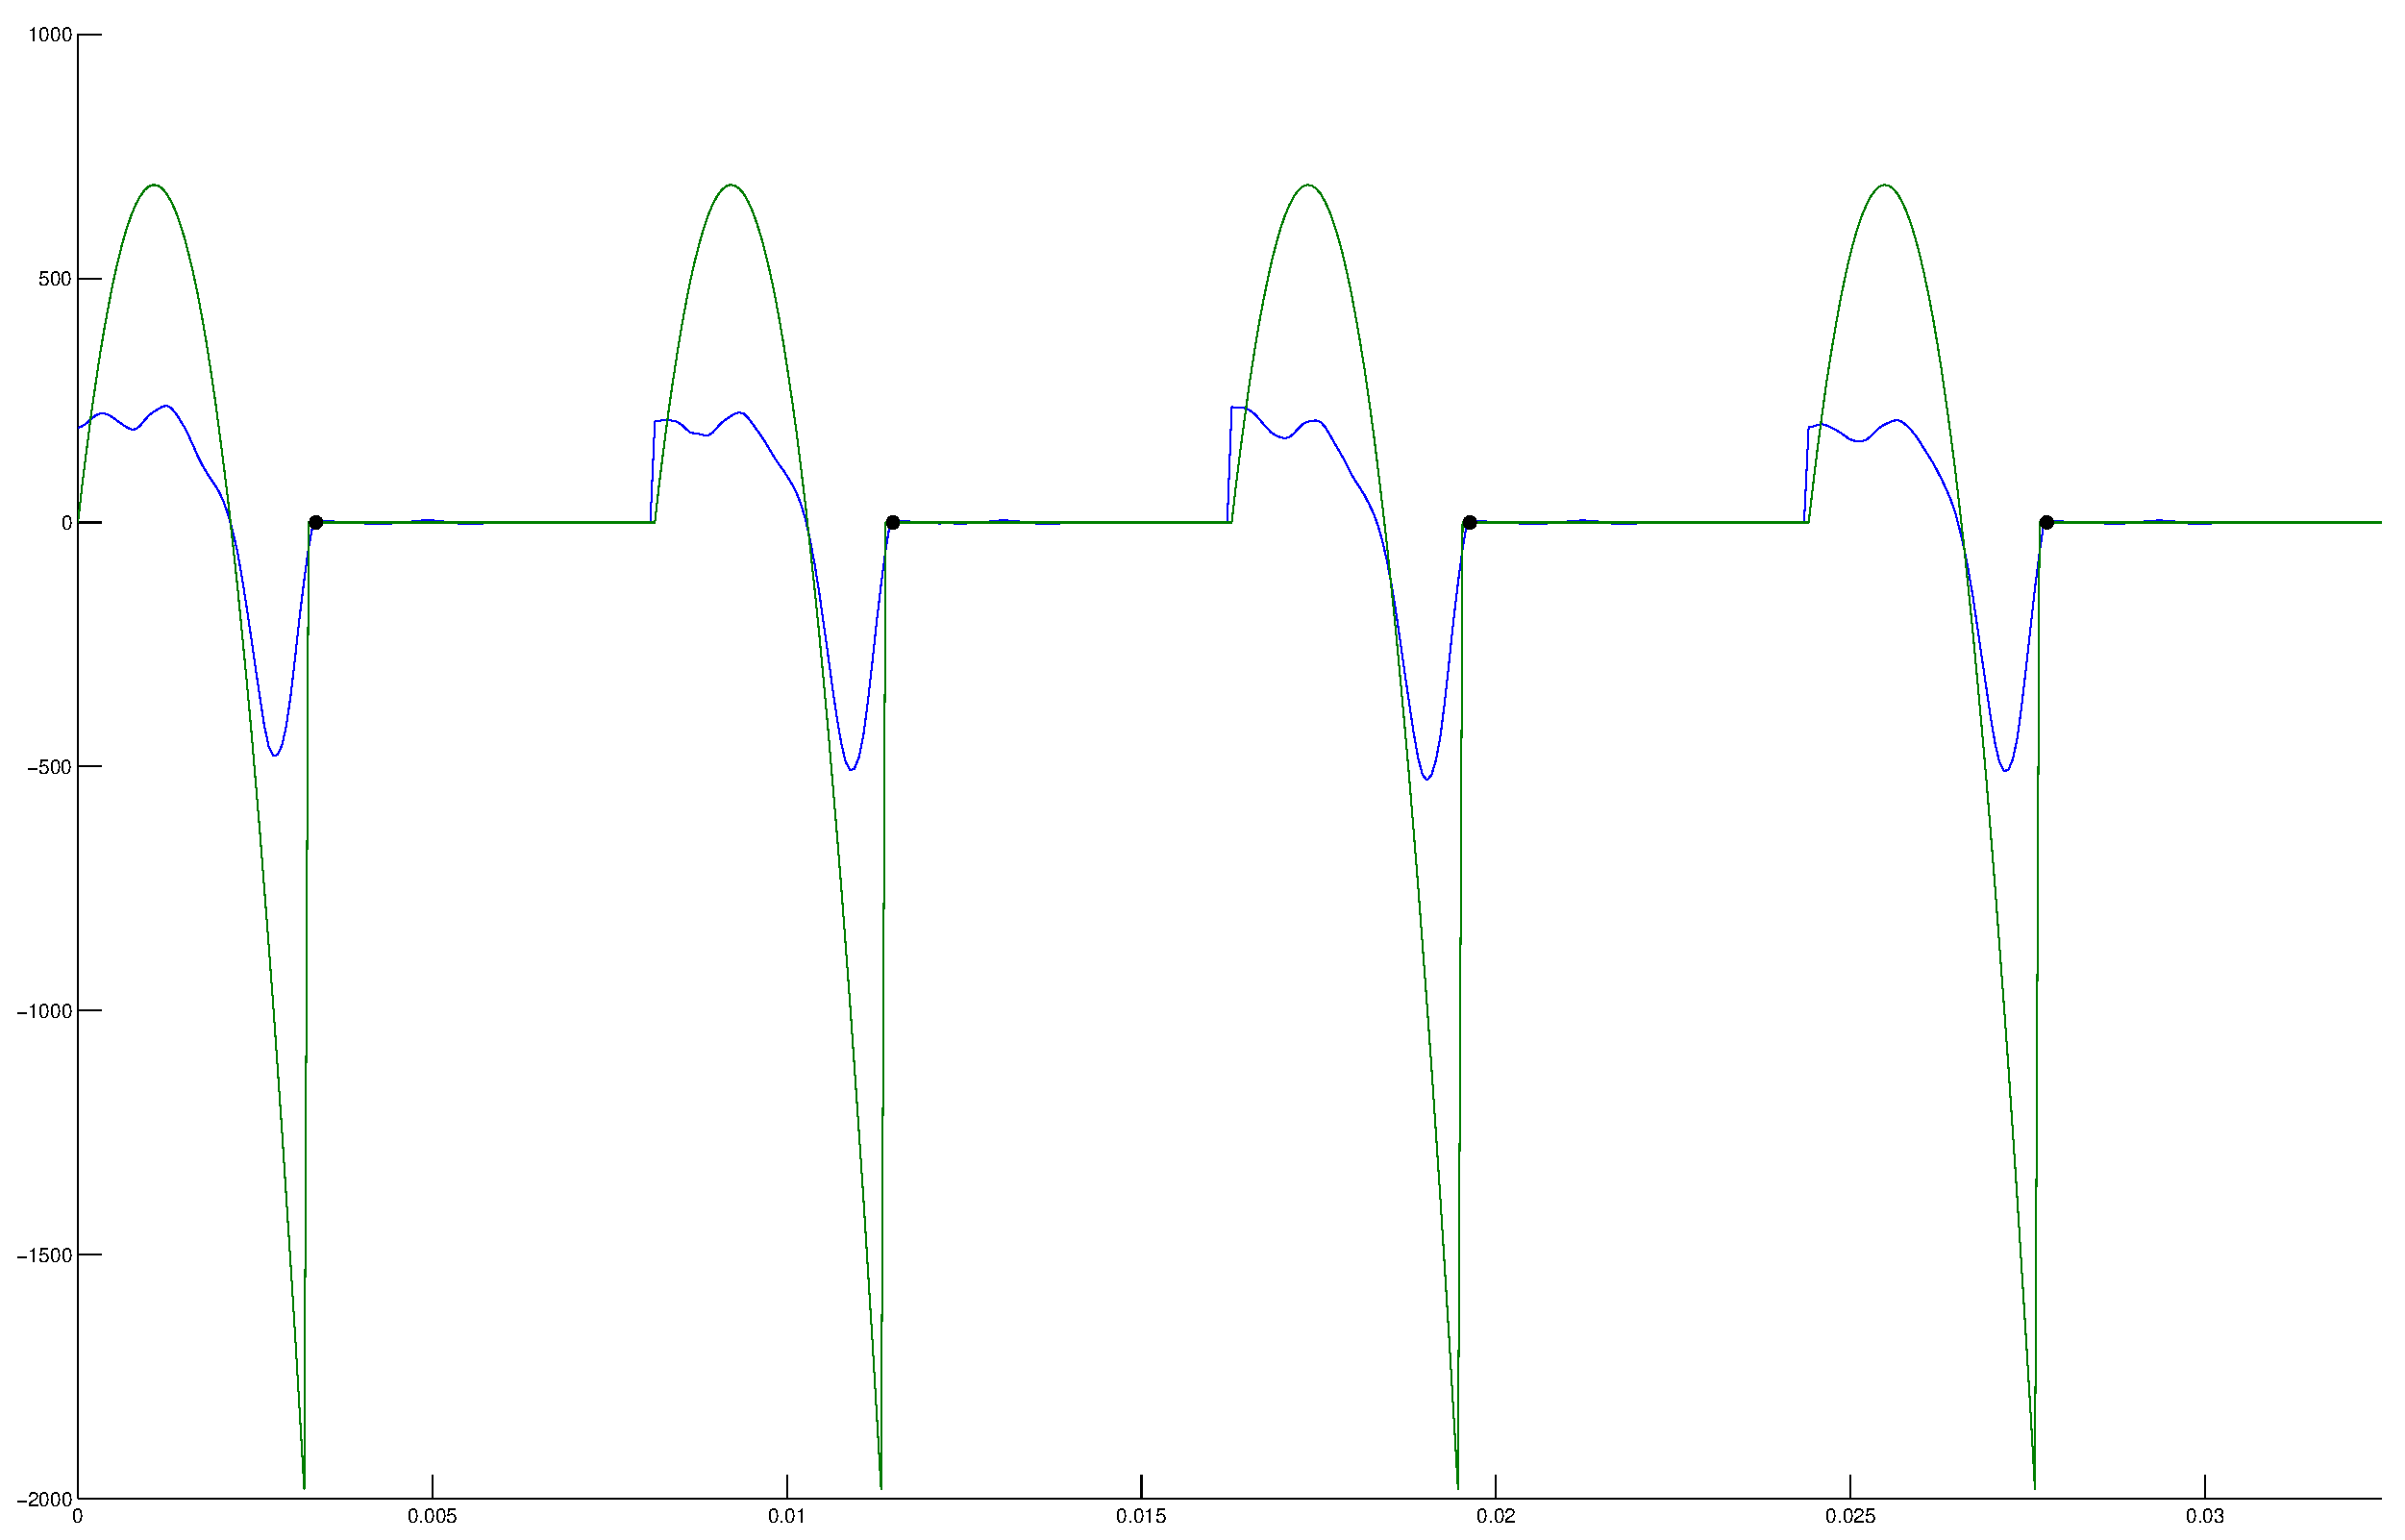
\includegraphics[scale=.2]{img/Approx_iter_wRef-4.eps}
 \caption{Iteration no.5.}
\end{center}
\end{figure}

\begin{figure}[H]
\begin{center}
 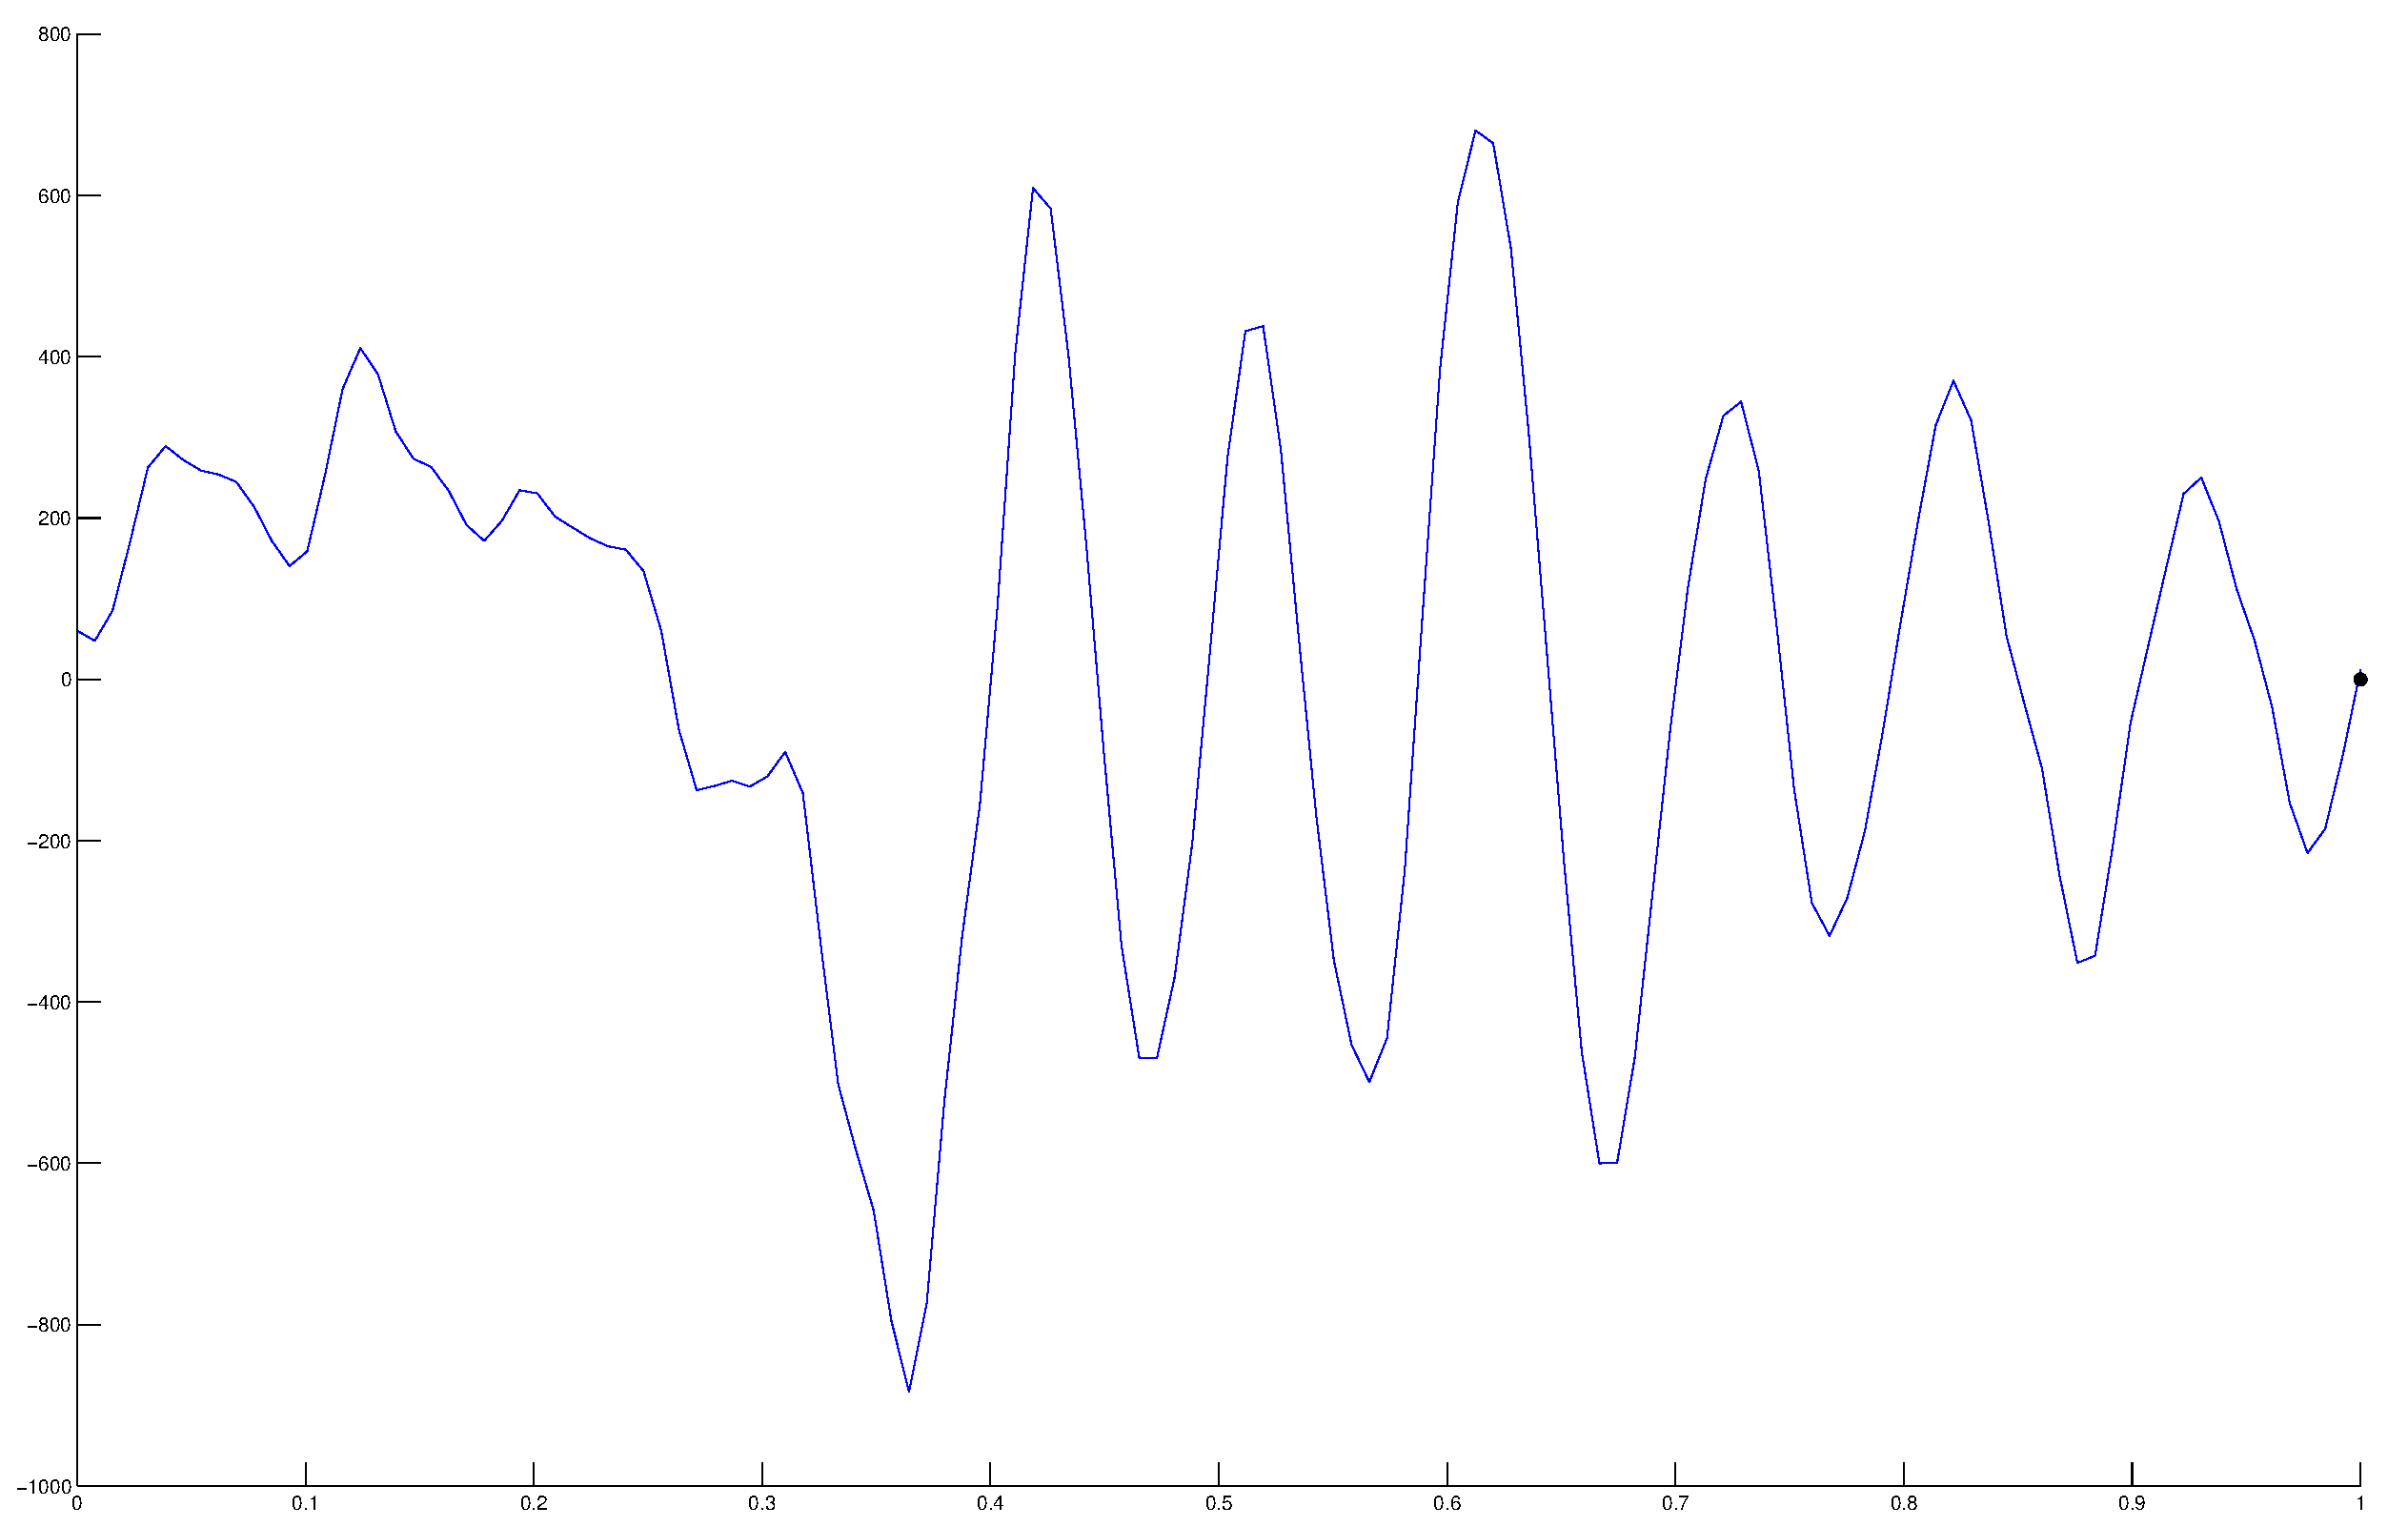
\includegraphics[scale=.2]{img/Approx_iter_onePer-1.eps}
 \caption{Iteration no.1}
 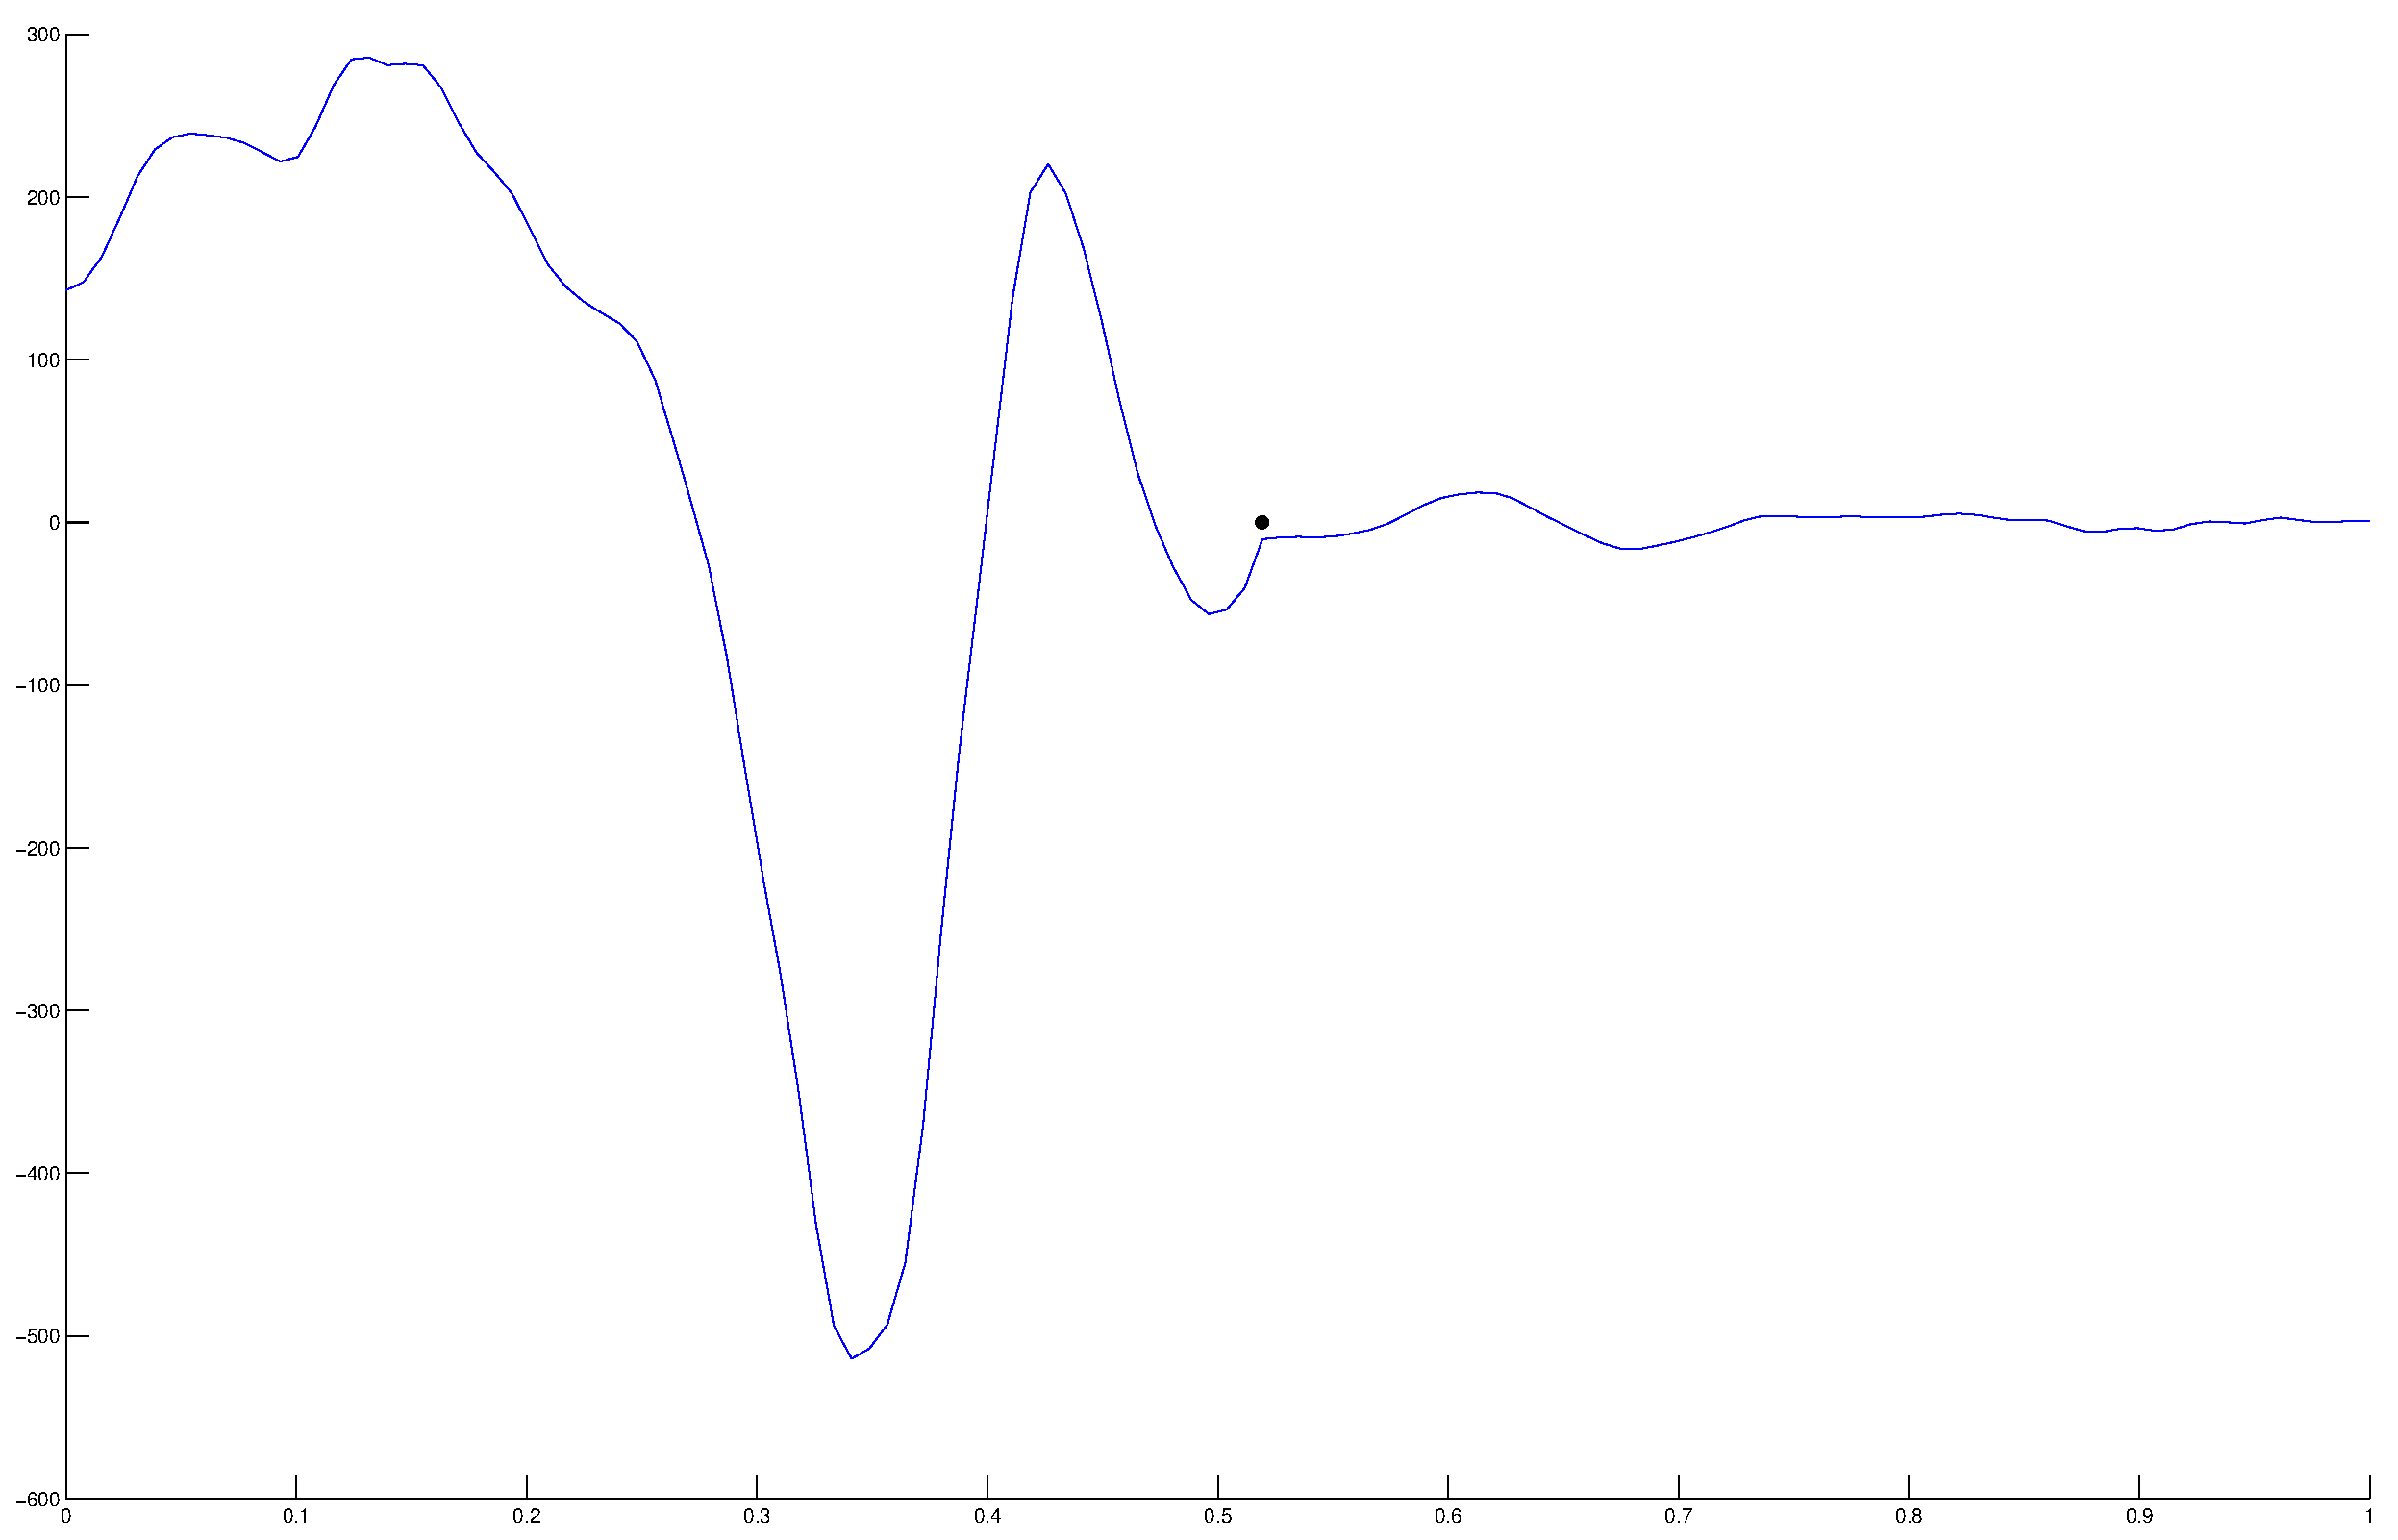
\includegraphics[scale=.2]{img/Approx_iter_onePer-2.eps}
 \caption{Iteration no.2}
 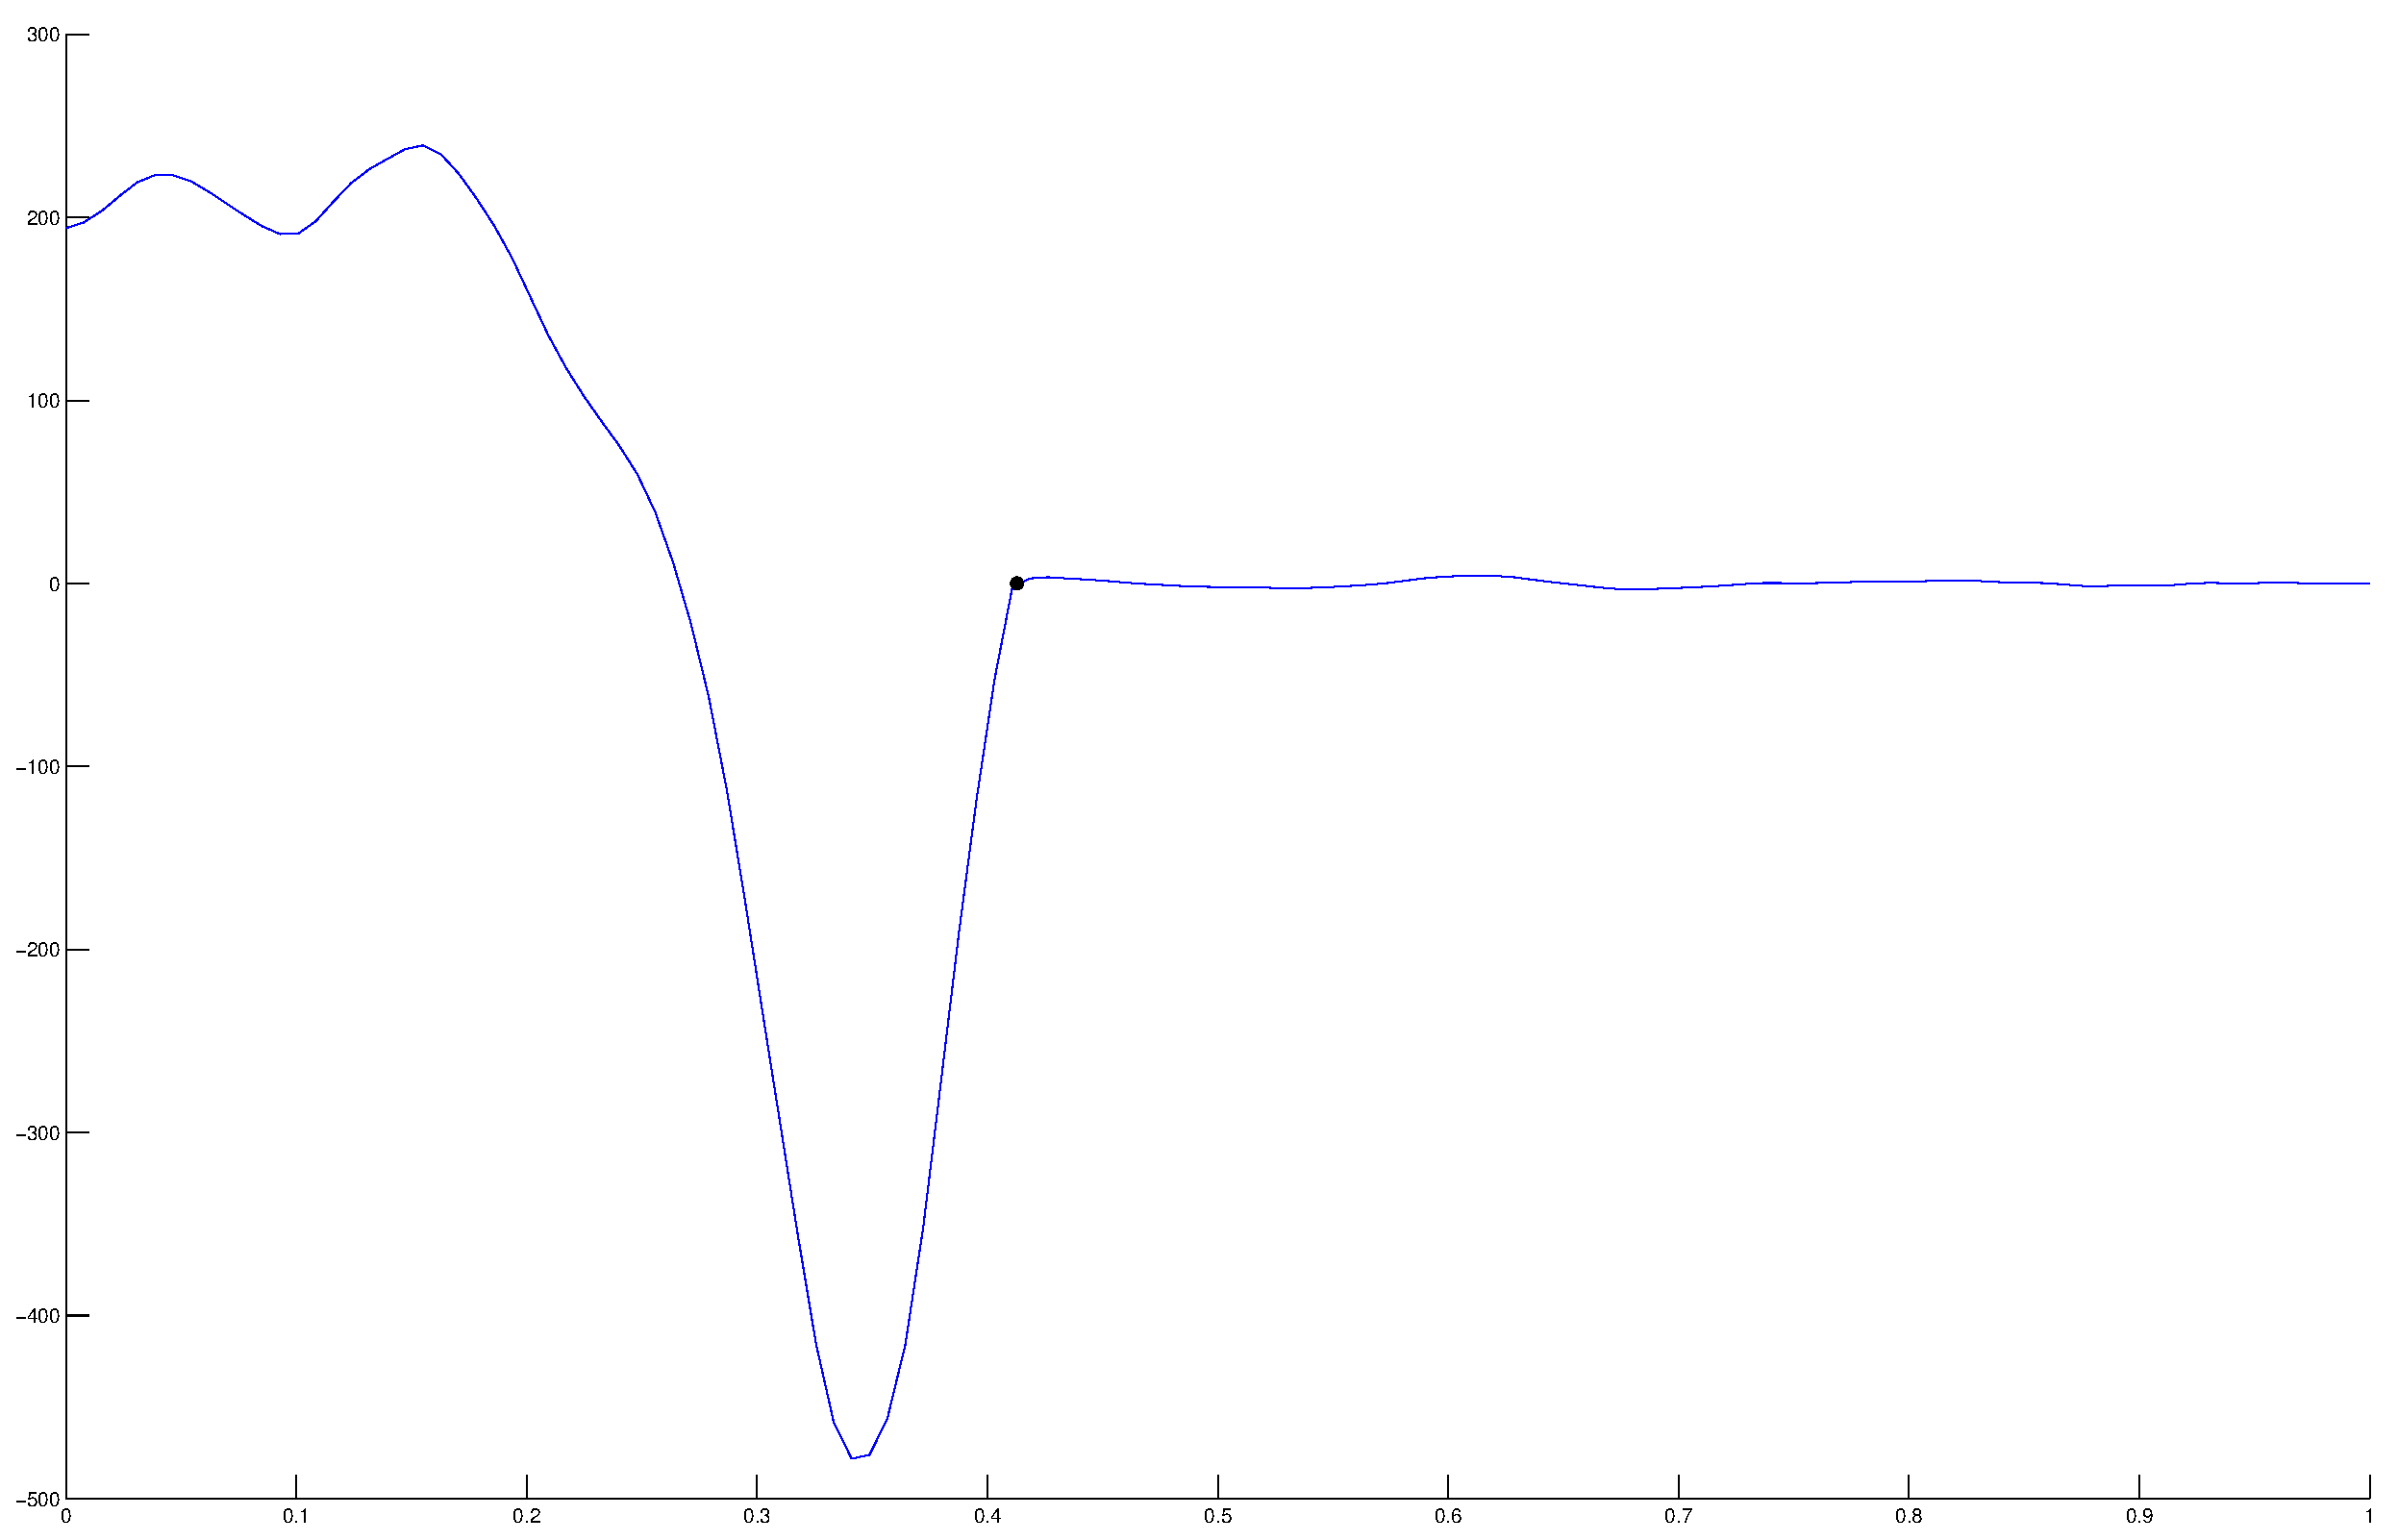
\includegraphics[scale=.2]{img/Approx_iter_onePer-4.eps}
 \caption{Iteration no.5}\label{fig:app2-end}
\end{center}
\end{figure}

\begin{figure}[H]
\begin{center}
 \caption*{In figures \ref{fig:app3-beginning} to \ref{fig:app3-end} the signal frequency is 123 Hz. The approximation algorithm acquired $Q_{guess} = 0.341$ at the end of the iterations, while the actual parameter $Q = 0.15$, relative error of the reconstruction $\approx$ 98.4\%, $\alpha \approx 8.3$. }
 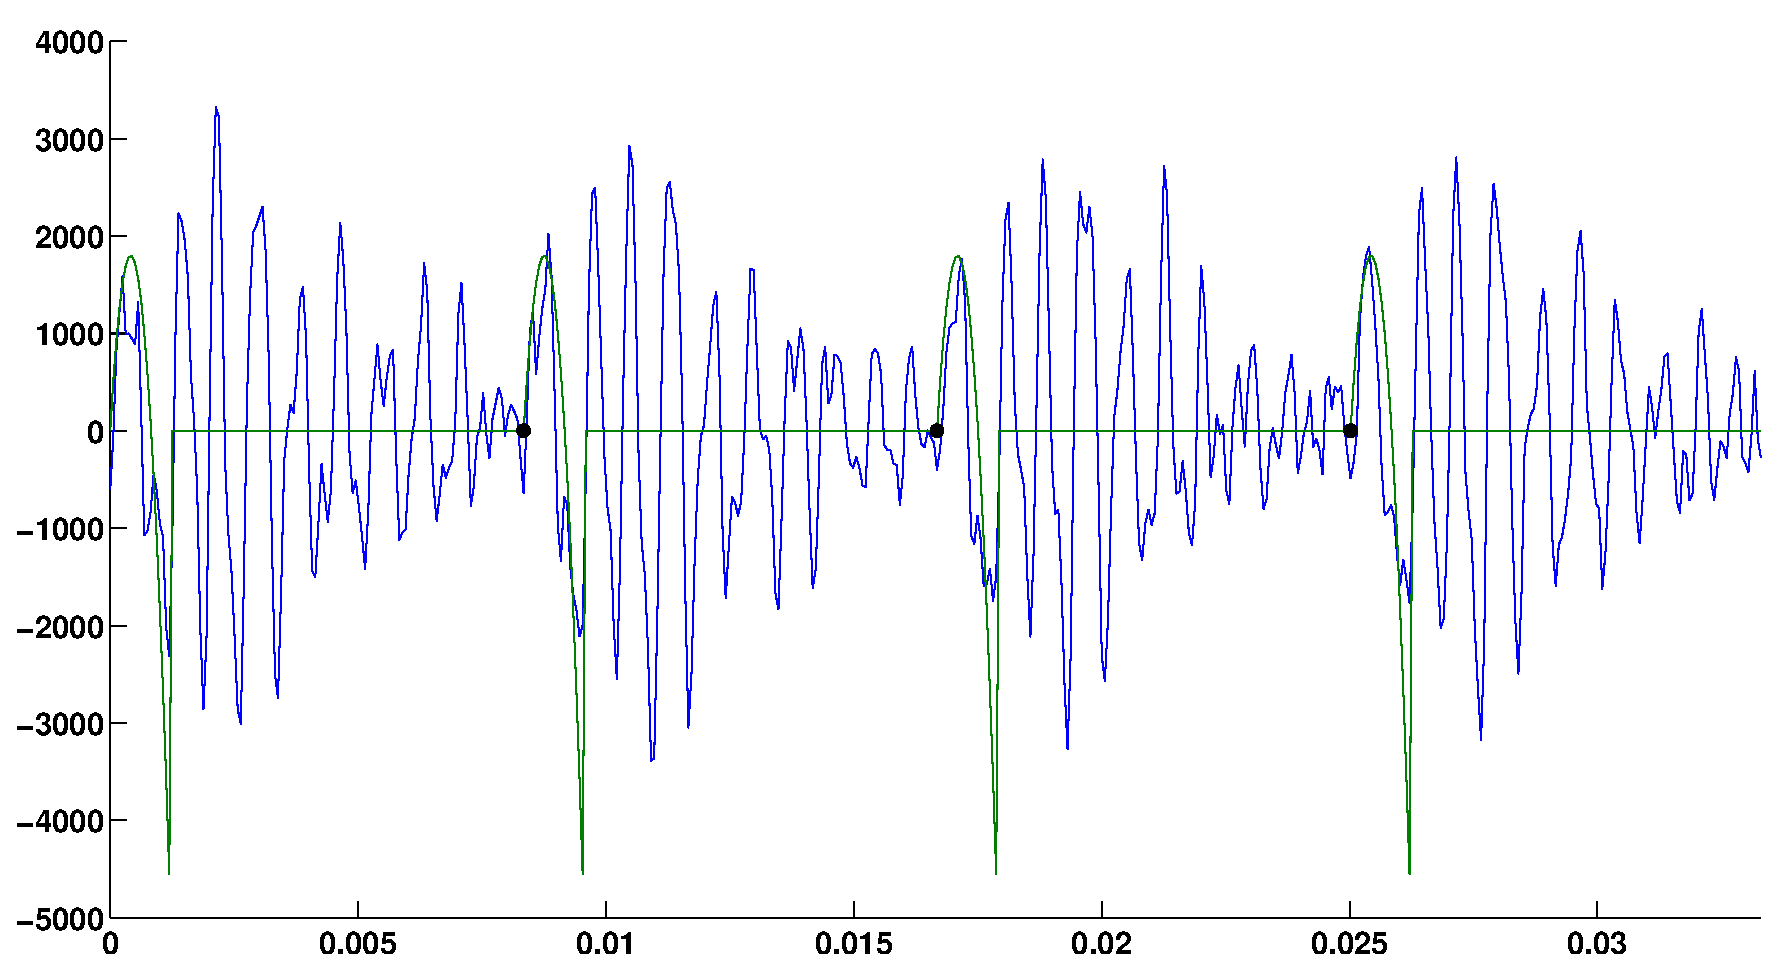
\includegraphics[scale=.35]{img/Approx_iter_wRef-v3-1.eps}
 \caption{Iteration no.1}\label{fig:app3-beginning}
 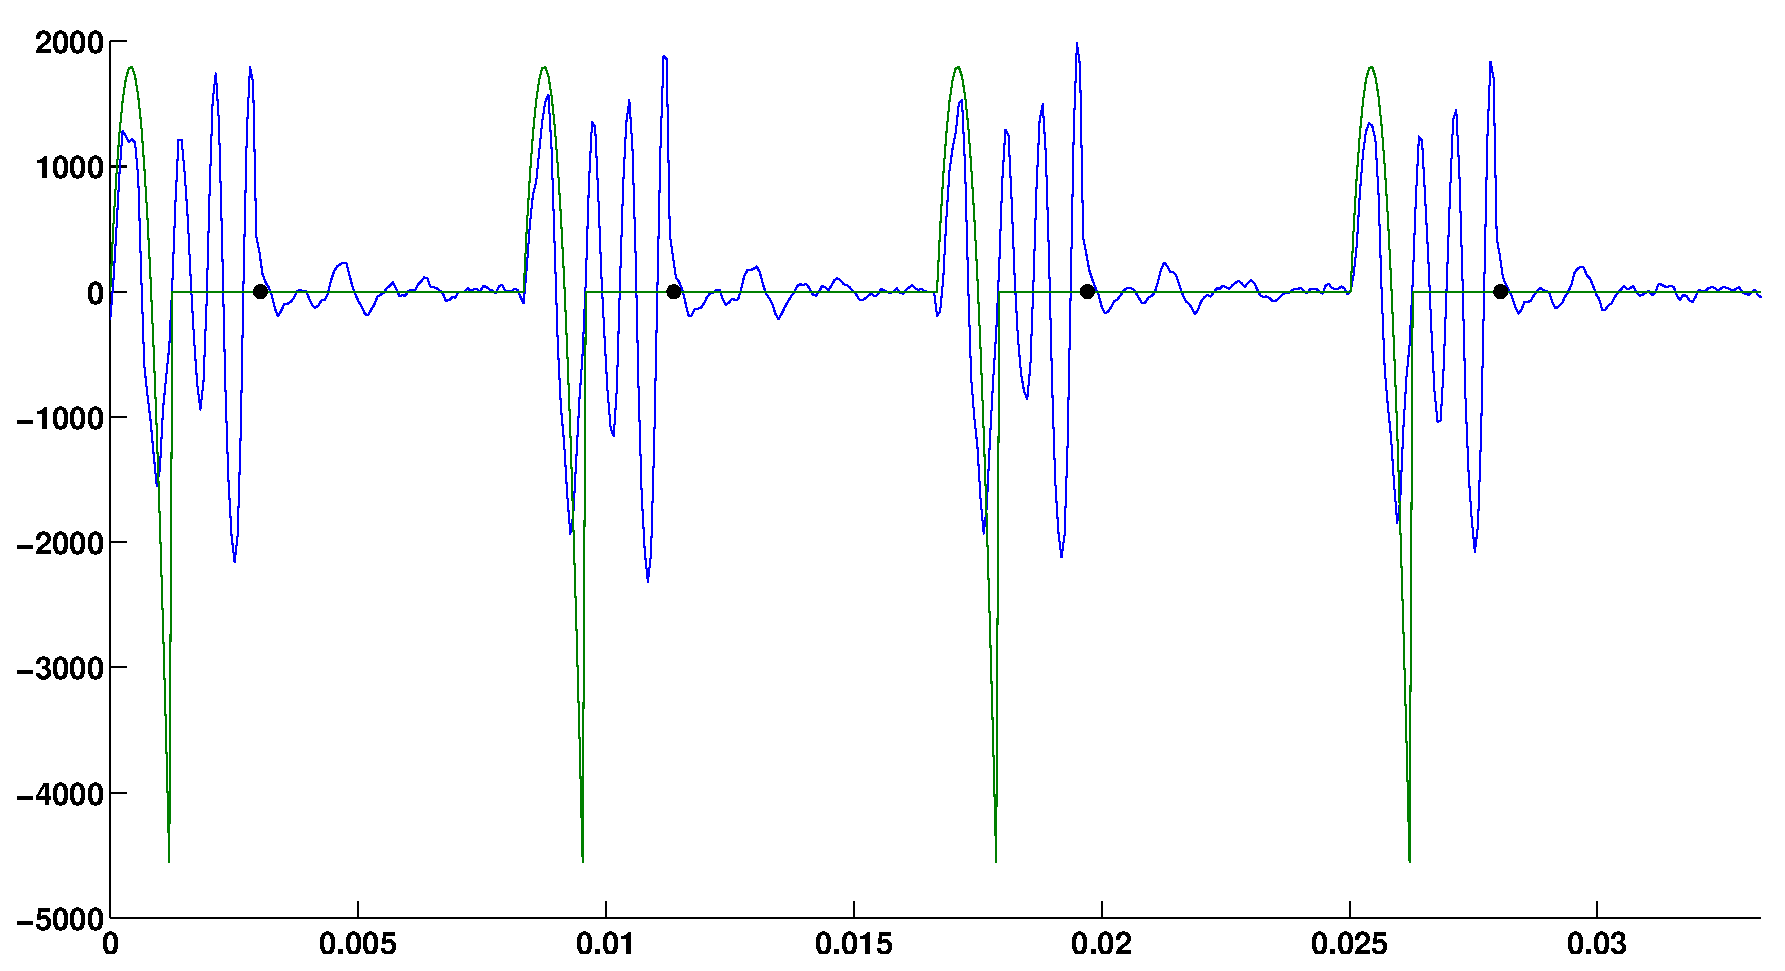
\includegraphics[scale=.35]{img/Approx_iter_wRef-v3-2.eps}
 \caption{Iteration no.2}
 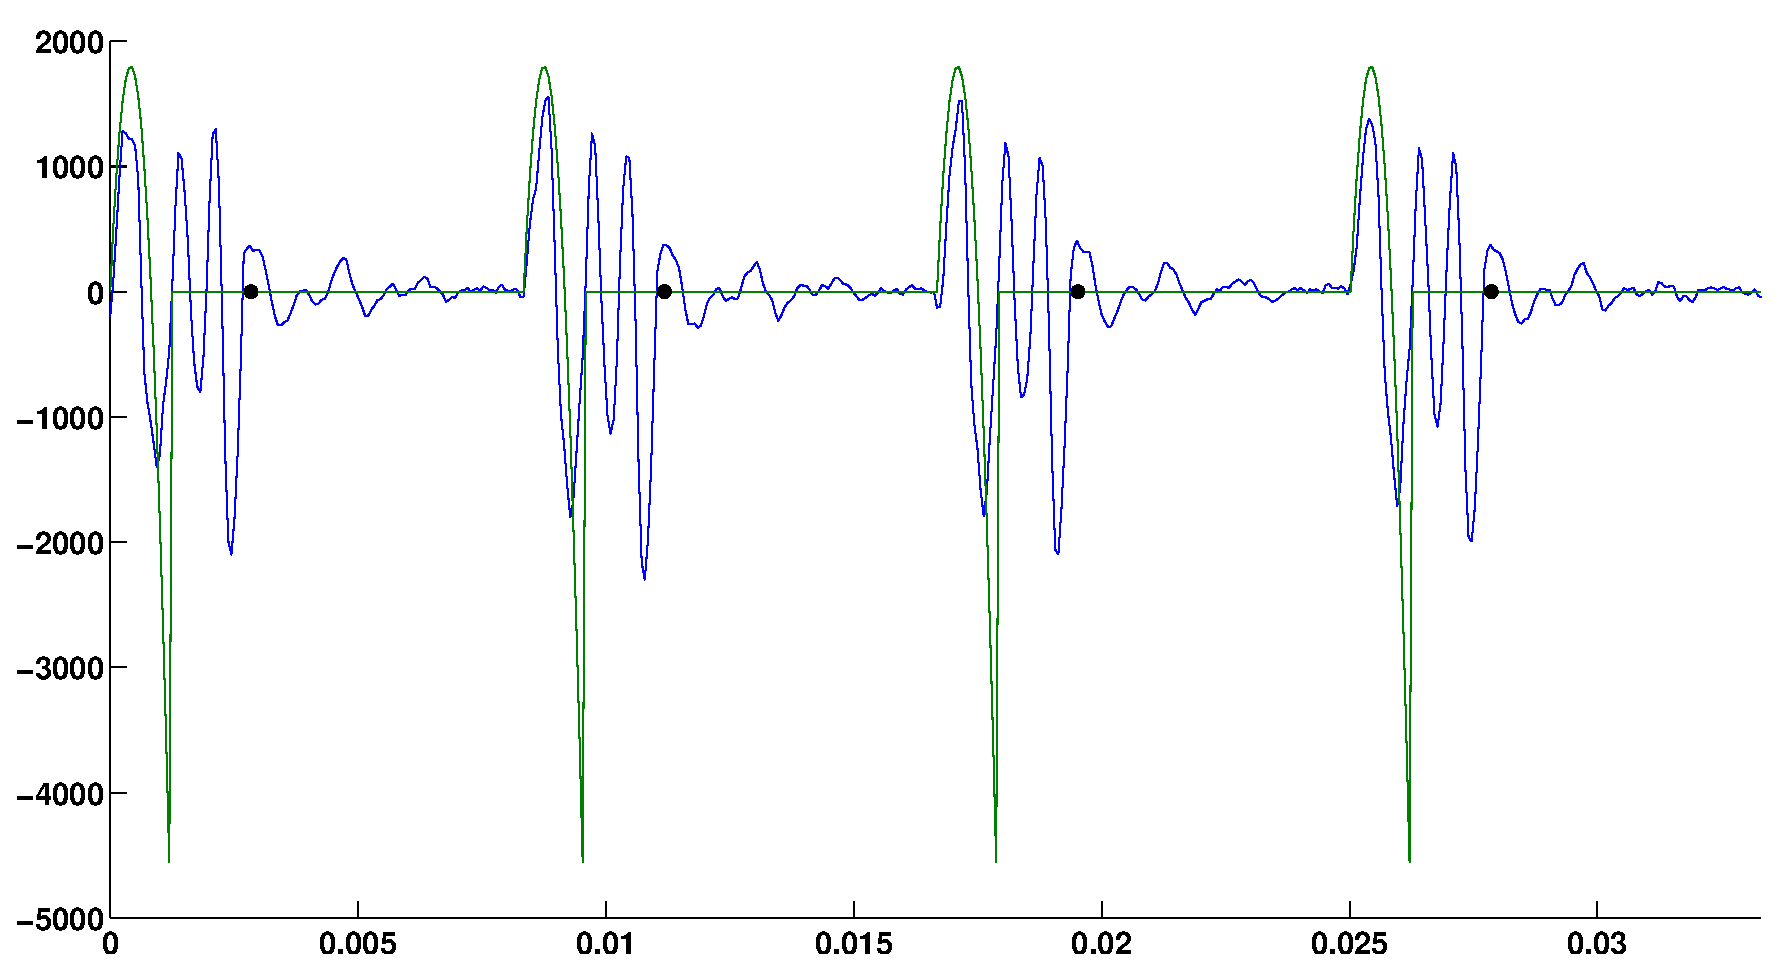
\includegraphics[scale=.35]{img/Approx_iter_wRef-v3-3.eps}
 \caption{Iteration no.5.}
\end{center}
\end{figure}

\begin{figure}[H]
\begin{center}
 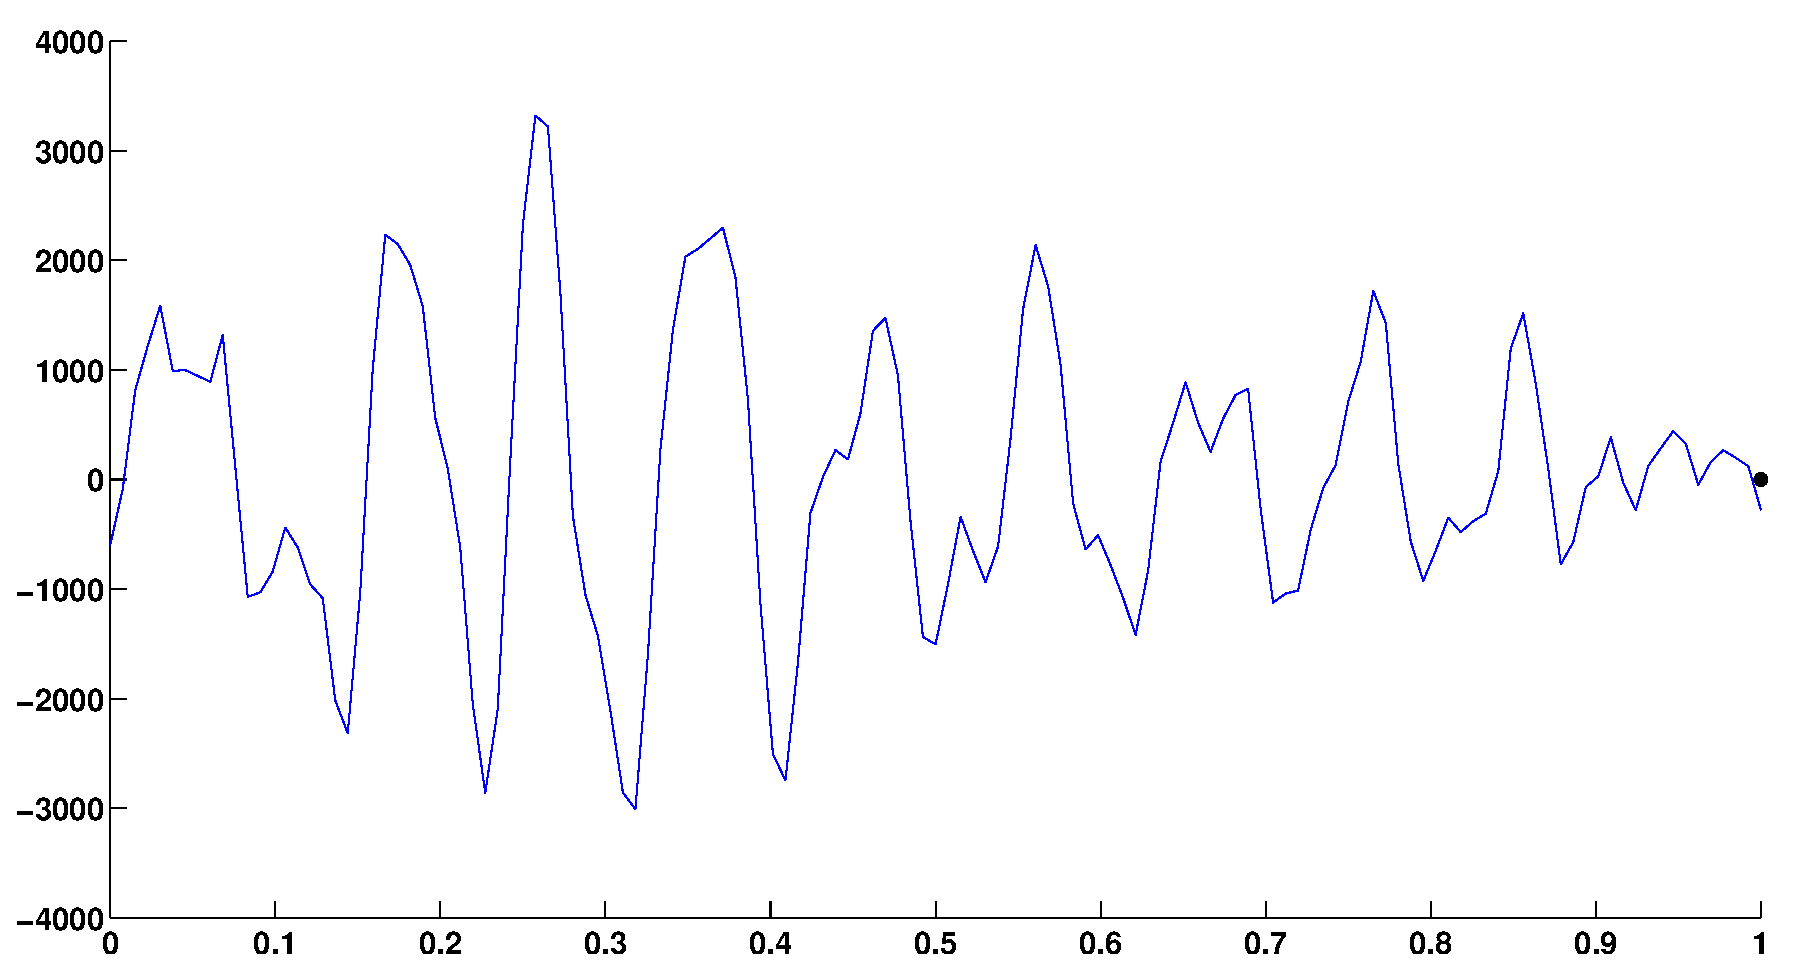
\includegraphics[scale=.35]{img/Approx_iter_onePer-v3-1.eps}
 \caption{Iteration no.1}
 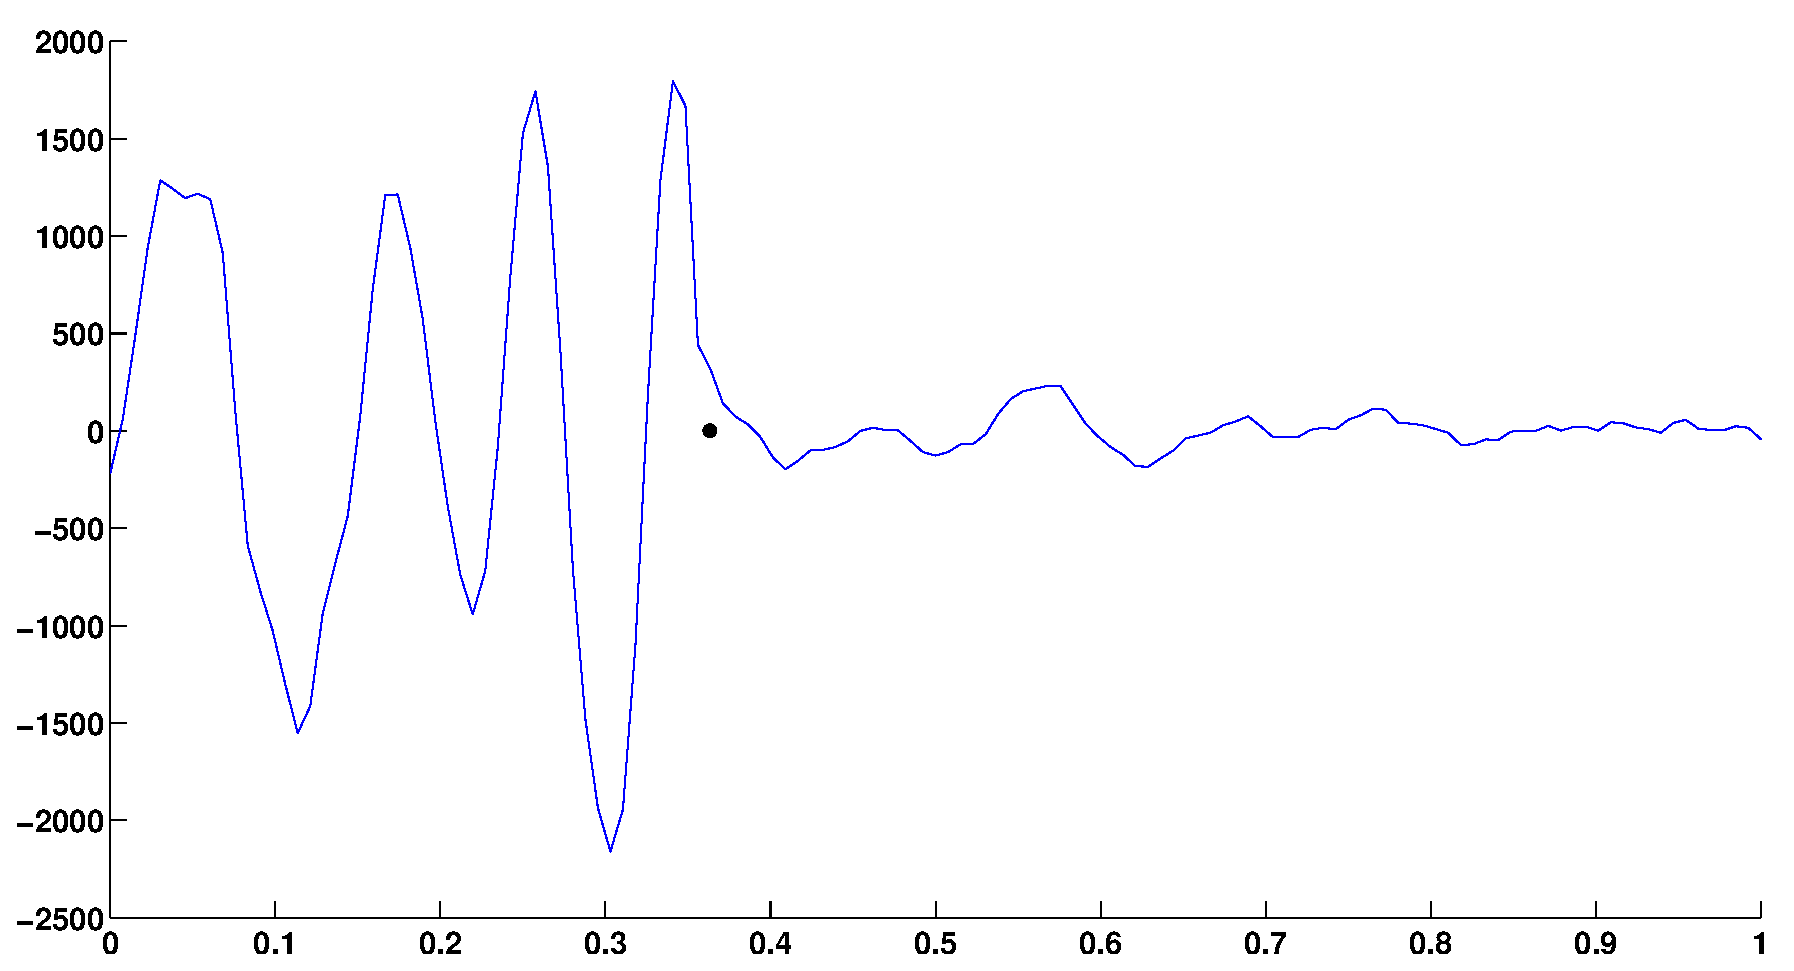
\includegraphics[scale=.35]{img/Approx_iter_onePer-v3-2.eps}
 \caption{Iteration no.2}
 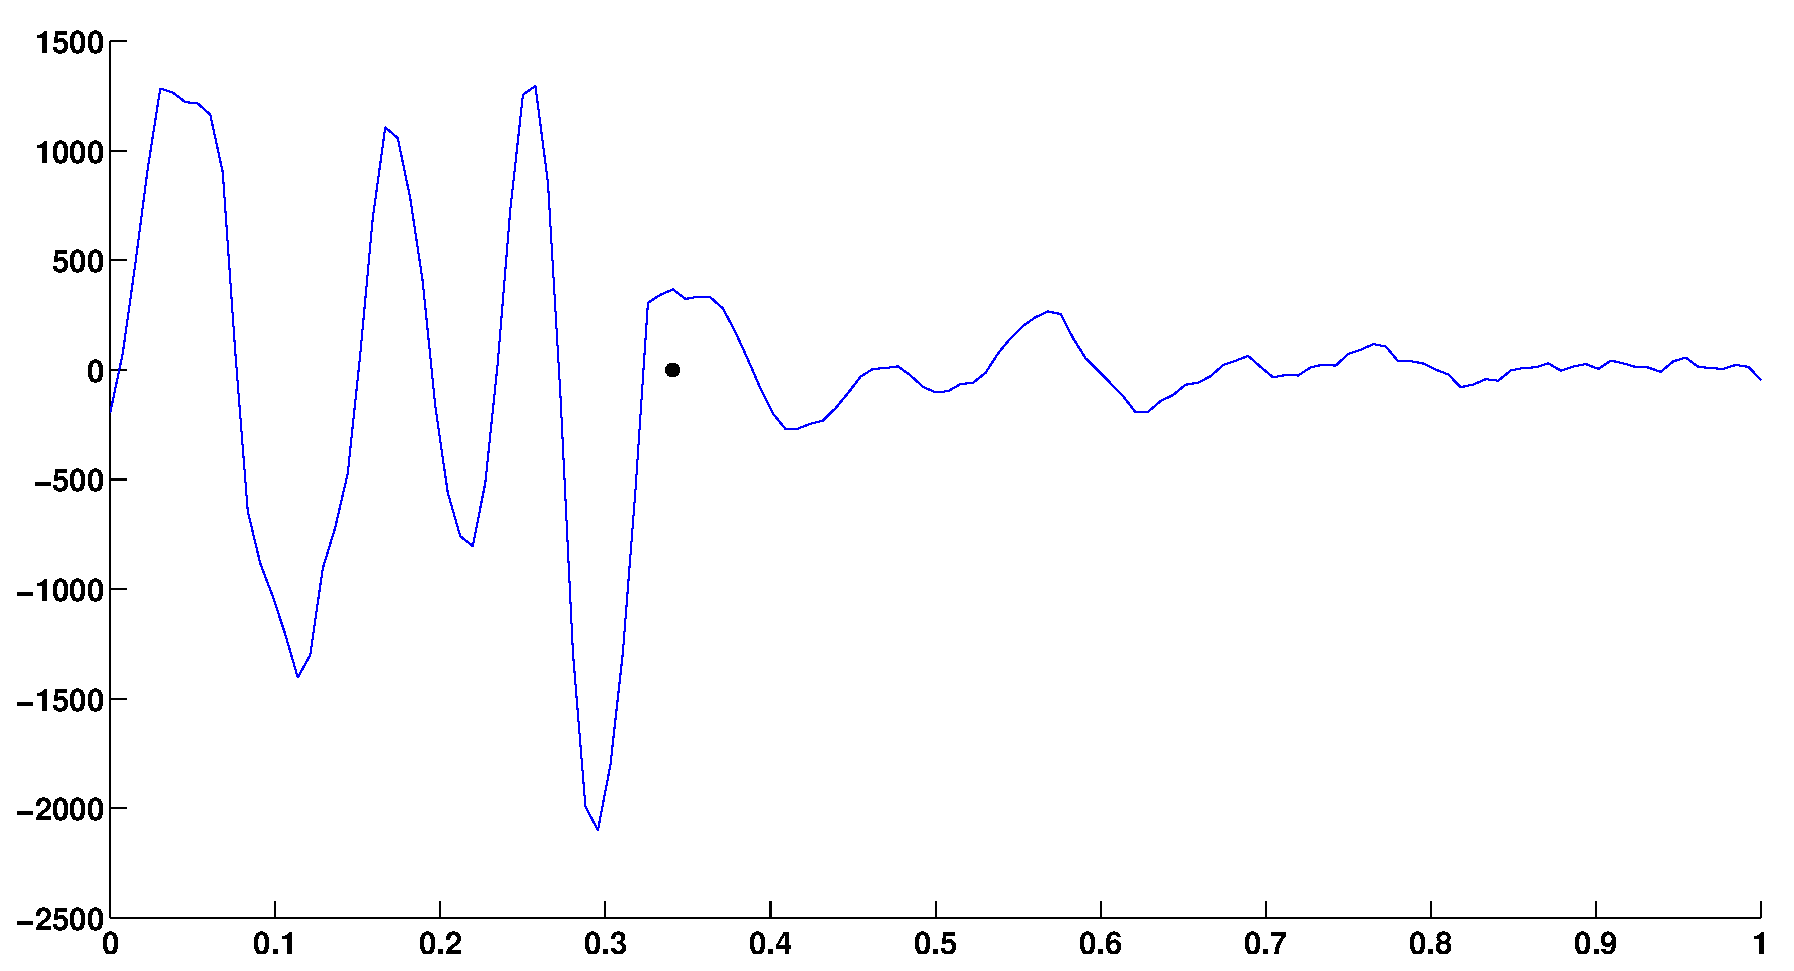
\includegraphics[scale=.35]{img/Approx_iter_onePer-v3-3.eps}
 \caption{Iteration no.5}\label{fig:app3-end}
\end{center}
\end{figure}

%----------------------Discussion---------------------
\section{Discussion}
\label{sec:discussion}

\subsection{Verification of the approximation method for \\approximating the Klatt-parameter}

In this section we will evaluate the efficiency of the approximation method for approximating the Klatt-parameter (explained in section \ref{sec:approxKlatt}). The convergence of the method is, in general, quite fast; the characteristics of the glottal excitation signal almost surely guarantees that the negative peak will dominate the oscillatory behaviour of a reconstruction computed with a too large Klatt-parameter guess.
This can be seen in figures \citeneeded. However, the algorithm will have no chance to recover from a situation where the oscillatory behaviour dominates over the negative peak (hence the previous "almost surely" formulation). This can be seen in figures \citeneeded. 

\subsection{Ill-posedness}'

As it can be seen from figures \ref{fig:naive-comparison_crime} and \ref{fig:naive-comparison_nocrime} the inverse problem to determine the glottal impulse is clearly \emph{ill-posed}. It can be seen that naïve inversion fails completely to achieve the shape of the glottal excitation signal, and thus a regularization method is required.

In this work the Tikhonov regularization strategy was chosen for solving the inverse problem. It can further be seen from figures \ref{fig:naive-comparison_crime} and \ref{fig:naive-comparison_nocrime} that when the same problem that failed with naïve inversion is solved with Tikhonov regularization the results are significantly better.

It must be noted that the situation displayed in figure \ref{fig:naive-comparison_crime} is done with inverse crime, which means that the same filter was used both in creating the data and in solving the inverse problem. This is the reason why the error of the reconstruction is so low; such low values could not be achieved with real data. The situation in figure \ref{fig:naive-comparison_nocrime} is a much better example of how reconstructions with real data could look like.

\subsection{Tikhonov regularization}
\label{sec:tikDiscussion}

Apart from the naïve inversions displayed in \cref{fig:naive-comparison_crime,fig:naive-comparison_nocrime} discussed above, all the reconstructions in \crefrange{fig:naive-comparison_crime}{fig:tik-5} are done with the Tikhonov regularization strategy. For all reconstructions the relative error was well below $75 \%$, which can be regarded as a good result.

As seen from the figures, the shape of the reconstruction is in all the cases clearly the same as in the original data, although the reconstruction is somewhat flattened. This is due to the high values of the regularization parameter used to compensate for the noise. The problem here is that although the \emph{sound} generated by the reconstruction is close to the original data the relative error of the reconstruction can become quite high; as the reconstruction is flattened it only affects the \emph{amplitude} of the generated sound as long as the \emph{shape} is unaltered. This is further discussed in \cref{sec:recQuality}.

Although the Tikhonov regularization strategy was found to work well for the glottal inversion problem, it relies heavily on many pieces of a-priori information. The information needed for the discussed method to work include the sound frequency and the Klatt-parameter of the glottal excitation signal used to generate the vowel sound. The sound frequency is an easy task to find from the measurement data, but the Klatt-parameter can be a harder task to find precisely.

If the Klatt-parameter is approximated too low (a too large part of a period of the reconstruction is suppressed by the penalty matrix, see \cref{sec:basis}) the peaks of the excitation signal would also be suppressed, thus ruining the reconstruction. If the value of the Klatt-parameter is approximated too high (smaller part of a period suppressed) a part of the reconstruction that should have the value 0 will become oscillatory (see example in \cref{fig:tooBigQ}). The latter would probably yield a better sound, as the characteristic shape of the glottal excitation signal would be established, although with some added noise. From this reconstruction the parameter could however be approximated again, as it will probably show in the reconstruction if the parameter value is estimated wrong. However, this means that the inversion process cannot be automated, as the Klatt-parameter must be found by hand.

Another way of tackling the problem of not knowing the Klatt-parameter exactly would be to alter the penalty matrix, for example by "smoothening" the transition from the discrete first derivative penalty to the suppressing part of the matrix. In this way the exact value would not be as important, but a good approximation would suffice. This is however beyond the scope of this study.

\begin{figure}[H]
\begin{center}
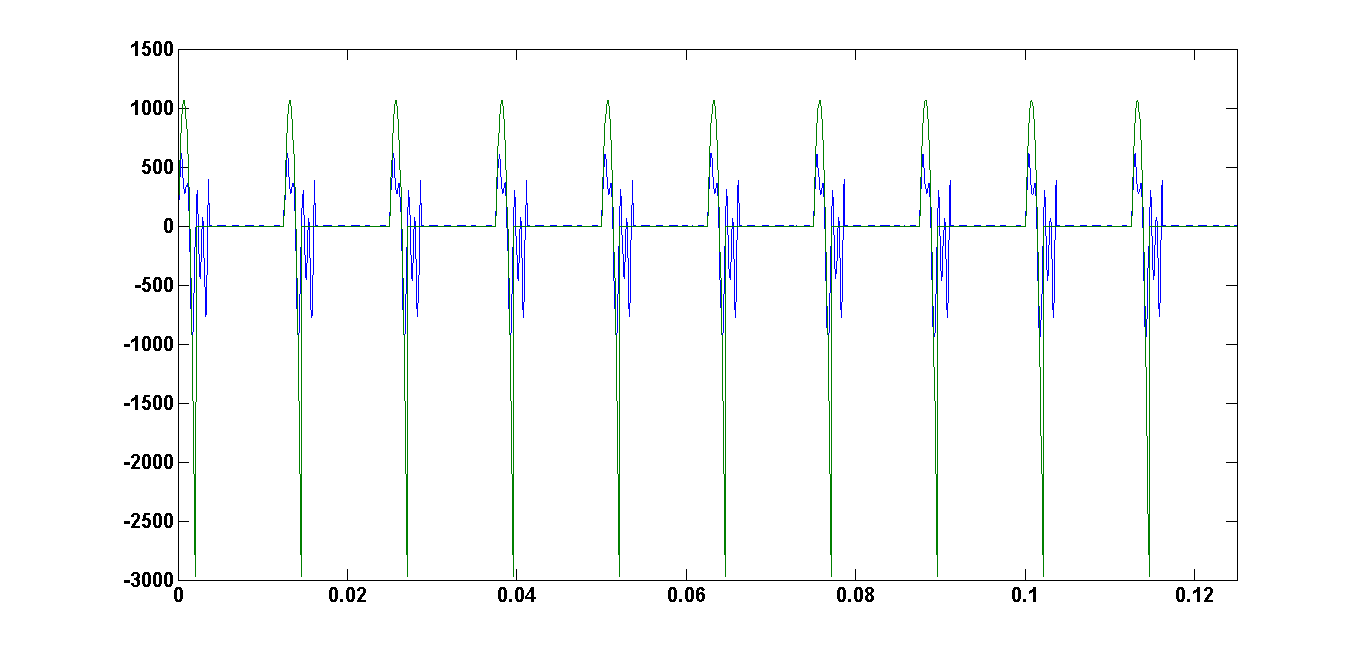
\includegraphics[scale=.3]{img/tooBigQ.png}
\end{center}
\caption{Example of a reconstruction done with a too big Klatt-parameter value.}
\label{fig:tooBigQ}
\end{figure}

\subsection{Morozov's discrepancy principle}
\label{sec:morozow}

The regularization parameters acquired with Morozov's discrepancy principle
yielded good results. As can be seen from \cref{fig:iter_comparison}, the reconstruction with a regularization parameter acquired with Morozov's discrepancy principle gave almost as good a reconstruction as with the best possible value of the parameter (in the sense of the values in the iteration) when using the relative error of the reconstructions as a reference point. The difference in the audio data was indistinguishable to the human ear.

Considering that the selection of the regularization parameter with Morozov's discrepancy principle works completely without the need of human interaction, the method selection can be regarded as a success for this particular problem. With an optimization of the noise estimation process (see \ref{sec:noiseEst}) potentially more accurate results can be acquired.

\subsection{Reconstruction quality}
\label{sec:recQuality}

As mentioned earlier in \cref{sec:tikDiscussion}, the relative error of the reconstruction compared with the original data might not be the perfect quantity to measure the quality of the reconstructions. As the values of the reconstruction signal are flattened, only the amplitude of sound generated by the reconstruction is affected, as long as the \emph{shape} of the signal is the same as for the original data. Therefore another way of measuring the error might be used.

The shape of the reconstruction signal could be compared by scaling the reconstruction and finding the smallest possible value for the relative error. This way only the shape, not the amplitude, of the reconstruction would matter. The shape error could thus be calculated as
\begin{equation}
\delta_{\text{shape}} = \min_{c \in \R} \left\{ \frac{\left\| \vc{g} - c T_{\alpha}(\vc{m}) \right\|_2}{\left\| \vc{g} \right\|_2} \right\} \cdot 100 \% ,
\end{equation}
where $\vc{g} \in \R^k$ is the original glottal excitation signal and $T_{\alpha}(\vc{m})$ is the reconstruction calculated from the noisy data $m$ with the regularization parameter $\alpha$.

However, it turned out that this way of comparing the reconstruction with the original data yielded similar results to the relative error. Therefore only the relative error was reported for the reconstructions.

\subsection{Further work}

In this work the inversion was done solely with simulated data. The same method might however be succesfully applied even to real recorded data. The vocal tract filter used in the inversion with the synthetic data is selected to simulate only an approximation of the real vocal tract filter, as the inversion uses another filter for the same vowel as what the data was created with. The situation with real data is not far from this starting point.

With the Tikhonov regularization strategy the reconstruction easily becomes oscillatory. As it was seen from the results in this work, to even out the oscillations the regularization parameter had to have a relatively high value. This in turn resulted in suppressed reconstructions. Also, the penalty matrix had to be heavily customized with Tikhonov regularization. Therefore, the inversion might work with the \emph{total variation} regularization strategy.\cite{samu} This could also be a good method of choise because it is planned to work well for piecewise constant functions, and a big part of the glottal excitation signal has the constant value zero.



%----------------------References---------------------
\newpage
\begin{thebibliography}{9}

\begin{footnotesize}
    
\bibitem{handbook}
    Abramowitz, M \& Stegun, I.A. (1965)
    \emph{Handbook of mathematical functions with formulas, graphs and mathenatical tables}
    New York, NY: Dover, p. 940
    
\bibitem{chi}
    Evans, M., Hastings, N. \& Peacock, B. (2000)
    \emph{Statistical distributions}.
    New York: Wiley, p. 57

\bibitem{fant}
    Fant, G., Liljencrants, J., Lin, Q., (1985).
    \emph{A four-parameter model of glottal flow}.
    STL-QPSR 26 (4), p. 1-13
    
\bibitem{fujisaki}
    Fujisaki, H., Ljungqvist, M., 1986.
    Proposal and evaluation of models for the glottal source waveform.
    In: Proc. IEEE International Conference on Acoustics, Speech and Signal Processing (ICASSP). Vol. 11. p. 1605–1608.
    
\bibitem{samu}
	Mueller, Jennifer L. \& Siltanen Samuli, (2012).
	\emph{Linear and Nonlinear Inverse Problems with Practical Applications}.
	SIAM, 1st edition.
    
\bibitem{NR}
    Press, W.H., Teukolsky, S.A., Vetterling, W.T. \& Flannery, B.P. (2007)
    \emph{Numerical Recipes: The Art of Scientific Computing}.
    New York: Cambridge University Press, 3rd edition, p. 362
    
\bibitem{digitalmodels}
    Rabiner, L. R., Schafer, R. W., (1987).
    \emph{Digital processing of speech signals}.
    Englewood Cliffs: Prentice-Hall, p. 38-107.

\bibitem{rosenberg}
    Rosenberg, A., (1971).
    \emph{Effect of glottal pulse shape on the quality of natural vowels}.
    Journal of the Acoustical Society of America 49 (2B), p. 583–590.
	
\bibitem{touda}
    Touda, K., (2007)
    \emph{Study on numerical method for voice generation problem}.
    PhD thesis.
    The University of Electro-Communications.


\end{footnotesize}

\end{thebibliography}

\end{document}



